
\documentclass[fontsize=10pt, oneside, DIV=calc]{scrartcl}
\scrollmode
\usepackage[
  pdfauthor={David Orban},
  pdftitle={Master Plan 4: Sustainable Multiplanetary Civilization Through Interplanetary AI},
  pdfsubject={CC BY 4.0 Licensed Work},
  pdfkeywords={Creative Commons, CC BY 4.0, David Orban, License}
  hidelinks
  pdfborder={0 0 0}
]{hyperref}
\usepackage{comment}
\usepackage{float}
\usepackage{fvextra}
\DefineVerbatimEnvironment{WrapVerbatim}{Verbatim}{breaklines=true}
\usepackage[T1]{fontenc}
\usepackage{lmodern}
\usepackage{xurl}
\usepackage{fontawesome5}
\usepackage{array,booktabs,tabularx}
\usepackage{pgf-pie}
\usepackage[most]{tcolorbox}
\usepackage[dvipsnames]{xcolor}
\usetikzlibrary{shadows}

\usepackage[export]{adjustbox}
\usepackage{pgfplots}
\usepackage{hyperref}
\usepackage{varwidth}

\usepackage{etoolbox}

% Locally disable PDF link borders in List of Illustrations
\let\oldnumberline\numberline
\renewcommand{\numberline}[1]{%
  \begingroup
    \hypersetup{pdfborder={0 0 0}}% no border for links in list
    \oldnumberline{#1}%
  \endgroup
}

\hypersetup{
    colorlinks=false,
    pdfborderstyle={/S/U/W 1},
    linkbordercolor=blue!70!black,
    breaklinks=true,
    pdfhighlight=/I,
    linktoc=all
}

\usepackage[normalem]{ulem}
\usepackage{moresize}
\usepackage{listings}
\usepackage{amsmath}

\usepackage[letterpaper,top=2cm,bottom=2cm,left=3cm,right=3cm,marginparwidth=1.75cm]{geometry} 

\usepackage[utf8]{inputenc}
\usepackage{amssymb}
\usepackage{forest}
\pgfplotsset{compat=1.18}
\usepackage{tikz}
\usetikzlibrary{positioning}
\usetikzlibrary{arrows}
\usepackage{graphicx}
\usepackage{wasysym}
\newcommand{\mycomment}[1]{}

\usepackage{FiraSans}
\renewcommand*\familydefault{\sfdefault}

\setkomafont{section}{\bfseries\Large\color[HTML]{000000}}
\setkomafont{subsection}{\bfseries\large\color[HTML]{000000}}
\pagecolor[HTML]{FFFFFF}
\color[HTML]{000000}

\usepackage{hyperref}

\title{Master Plan 4: Sustainable Multiplanetary Civilization Through Interplanetary AI}
\author{David Orban}
\date \today

\begin{document}
\setcounter{page}{2}
\maketitle
\begin{center}
\textbf{Version 1.0}
\end{center}

\begin{center}
\href{https://davidorban.com}{\texttt{davidorban.com}} \quad | \quad
\href{https://masterplan4.org}{\texttt{masterplan4.org}}
\end{center}

\section*{Executive Summary}
\addcontentsline{toc}{section}{Executive Summary}

Establishing a sustainable human presence beyond Earth is essential for our civilization's long-term viability. Mars is the most accessible planetary body for initial large-scale settlement. This report presents Master Plan 4, a strategic roadmap detailing the phased development of a sustainable, interplanetary AI-driven civilization centered on Mars. The primary objective is to construct the foundational infrastructure and economic engine required for self-sufficiency and future expansion.

The plan relies on the development of a Terawatt-scale solar-based Martian energy grid and the subsequent deployment of Colossus, a Terawatt-scale AI data center. This computational capacity supports human-driven and AI-augmented discovery, designed to accelerate scientific and engineering breakthroughs and drive the economy of the Martian colony.

The name derives Master Plan 4 follows the previously published Master Plans 1, 2, and 3 by Tesla, extending the concept to encompass not only solar power, batteries, and humanoid robots, but also to fully reusable interplanetary spacecraft, and AI data centers.

\section*{Disclaimer}
\addcontentsline{toc}{section}{Disclaimer}
This document is a speculative foresight report, outlining hypothetical technological, economic, and governance scenarios based on current trends and public knowledge. It is not an official plan or commitment by any real-world entity.

Created through Human–AI collaboration, the report integrates input from tools including ChatGPT, Gemini, Claude, Grok, and DeepWriter, under the direction of David Orban. It does not constitute medical, legal, financial, or professional advice. References to real individuals or organizations are illustrative only. Consult qualified experts for real-world decisions.

\section*{License}
\addcontentsline{toc}{section}{License}
\vspace{-1em}
This work by David Orban is licensed under the 
\href{https://creativecommons.org/licenses/by/4.0/}{Creative Commons Attribution 4.0 International License (CC BY 4.0)}. You are free to share — copy and redistribute the material in any medium or format; adapt — remix, transform, and build upon the material for any purpose, even commercially; under the following terms: attribution — you must give appropriate credit, provide a link to the license, and indicate if changes were made.
        
\newpage
\begingroup
\setcounter{tocdepth}{5}
\hypersetup{hidelinks}
\tableofcontents
\endgroup
\newpage

\section*{I. Report Overview and Objectives}

\addcontentsline{toc}{section}{I. Report Overview and Objectives} 


\subsection*{}

\subsection*{1. Introduction and Core Objective}

\addcontentsline{toc}{subsection}{1. Introduction and Core Objective} 


\medskip

\noindent
Master Plan 4 presents a strategic roadmap for the phased development of an interplanetary civilization beginning on Mars. The plan's core objective is to accelerate scientific discovery and establish a self-sustaining, AI-driven economy beyond Earth. This is centered on deploying a terawatt (TW)-scale artificial intelligence data center, designated `Colossus', on the Martian surface. This facility serves as the primary engine for the interplanetary endeavor.

\medskip

\noindent
The rationale for this undertaking is twofold. Firstly, situating a computational facility of this magnitude on Mars leverages the Martian environment, including its ambient temperatures, which aid in cooling efficiency for high-density computing hardware. Secondly, the physical distance from Earth requires a high degree of local autonomy, necessitating advanced AI for operational management, decision-making, and scientific research. 

NASA's Moon to Mars objectives outline foundational infrastructure for initial human exploration, including surface power and communications systems.\footnote{National Aeronautics and Space Administration, ``Moon to Mars Objectives,'' September 2022, p. 9,\href{https://www.nasa.gov/wp-content/uploads/2022/09/m2m-objectives-exec-summary.pdf}\url{https://www.nasa.gov/wp-content/uploads/2022/09/m2m-objectives-exec-summary.pdf}}. This plan builds upon these requirements, scaling them to support TW-level operations.

\medskip

\noindent
Establishing the Martian Energy Grid, projected to reach TW-scale primarily through solar power generation, is a prerequisite for Colossus Deployment. While initial estimates for solar panel area exceed 8,500 km²\footnote{J. S. McNatt, ``Photovoltaics and Power to Support NASA’s Moon to Mars Objectives,'' presented at the 28th Space Photovoltaic Research and Technology Conference, Cleveland, Ohio, Sep. 4, 2024, p. 5. Available: 







\href{https://ntrs.nasa.gov/api/citations/20240010682/downloads/PV\%20and\%20Power\%20to\%20Support\%20NASA\%20M2M.pdf}\url{https://ntrs.nasa.gov/api/citations/20240010682/downloads/PV\%20and\%20Power\%20to\%20Support\%20NASA\%20M2M.pdf}}, potentially approaching 30,000 km² when accounting for Martian environmental factors and continuous power needs, this infrastructure is fundamental. The power architecture for Mars is evolving; fission surface power is identified as a leading candidate due to its resilience to dust storms\footnote{National Aeronautics and Space Administration, ``Moon to Mars Architecture Definition Document (ESDMD-001) – Revision B.1,'' December 13, 2024, p. 163, 







\href{https://www.nasa.gov/wp-content/uploads/2024/12/esdmd-001-add-rev-b.pdf?emrc=5ffbf4}\url{https://www.nasa.gov/wp-content/uploads/2024/12/esdmd-001-add-rev-b.pdf?emrc=5ffbf4}}. Colossus operation is projected to drive Resource Valorization, converting local Martian resources and computational power into tangible economic value. This value creation centers on the monetizable outputs of AI-driven scientific discovery, engineering optimization, and resource processing.

\medskip

\noindent
This process initiates Exponential Scaling across the Martian settlement, encompassing population growth, infrastructure expansion, scientific output, and economic productivity. The synergy of these elements forms the Systemic Expansion Engine, designed to propel the endeavor towards self-sustainability and beyond. Master Plan 4 encompasses accelerating scientific discovery via AI research, developing a novel computational resource economics framework, and strategic expansion into the asteroid belt and outer planets, using Mars as the central AI and manufacturing hub. Initial mission mass requirements for human Mars exploration in Low Earth Orbit are estimated at 900 to 1,300 metric tons\footnote{Jones, H. W. (2016). Humans to Mars Will Cost About ``Half a Trillion Dollars'' and Life Support Roughly Two Billion Dollars. \textit{46th International Conference on Environmental Systems}, Vienna, Austria. ICES-2016-111. Retrieved from 







\href{https://ntrs.nasa.gov/api/citations/20200000973/downloads/20200000973.pdf}\url{https://ntrs.nasa.gov/api/citations/20200000973/downloads/20200000973.pdf}}, indicating the scale of initial Earth-based support required.

\medskip

\noindent
Autonomous governance structures on Mars are a critical component of this plan. Given communication latency with Earth\footnote{Edwards, B. L. (2024, November). Unlocking New Capabilities in Space Communications for NASA. NASA Space Technology Mission Directorate. Retrieved from 







\href{https://ntrs.nasa.gov/api/citations/20240013248/downloads/Edwards\%20Presentation\_Ver\%202.pdf}\url{https://ntrs.nasa.gov/api/citations/20240013248/downloads/Edwards\%20Presentation\%20Ver\%202.pdf}}, local decision-making authority is essential for operation and growth. This governance framework will develop incrementally, in parallel with the Martian population and its capabilities. It will progressively address the ethical and legal considerations of integrating advanced AI and robotic entities into Martian society, including the potential for their progressive acquisition of rights as their roles evolve\footnote{Lucas-Stannard, P., \& Lasslop, A. (Eds.). (2006). \textit{Mars Settlement and Society Working Group Report}. Next Generation Exploration Conference 2006, p. 5. 







\href{https://ntrs.nasa.gov/api/citations/20070008279/downloads/20070008279.pdf}\url{https://ntrs.nasa.gov/api/citations/20070008279/downloads/20070008279.pdf}}. The following sections detail the technical, economic, and operational strategies to realize this vision, presenting a roadmap for interplanetary expansion and establishing a new branch of human (and post-human) civilization.



\begin{figure}[H]
  \centering
  \noindent
  \begin{minipage}{\textwidth}
    \centering
    \adjincludegraphics[
      max size={\textwidth}{0.9\textheight},
      keepaspectratio
    ]{images/inline-diagram-5899905249}
    \caption{A high-level relationship diagram illustrates the core entities of Master Plan 4: Earth, Mars, the Colossus AI Data Center, the Interplanetary Economy, Scientific Discovery, and Autonomous Governance. Lines indicate key dependencies and interactions, such as Earth's role in initial supply, Colossus powering the economy and science, and governance overseeing operations.}
  \end{minipage}
\end{figure}

\begin{comment}
@startuml
!theme carbon-gray
scale 1.6

skinparam defaultFontColor black
skinparam backgroundColor white


title ``Master Plan 4: Core Entities''

skinparam componentStyle rectangle

component ``Earth'' as Earth
component ``Mars'' as Mars

component ``Colossus\nAI Data Center'' as Colossus
component ``Interplanetary\nEconomy'' as Economy
component ``Scientific\nDiscovery'' as Science
component ``Autonomous\nGovernance'' as Governance

Earth --> Mars : ``Initial Supply''

Mars -down-> Colossus : ``Hosts''
Mars -down-> Economy : ``Hosts''
Mars -down-> Science : ``Hosts''
Mars -down-> Governance : ``Hosts''

Colossus --> Economy : ``Powers\nEconomy''
Colossus --> Science : ``Drives\nScience''

Science --> Economy : ``Generates\nValue''

Governance -left-> Mars : ``Oversees\nMars Hub''

@enduml
\end{comment}





            
\section*{II. Foundational Principles}

\addcontentsline{toc}{section}{II. Foundational Principles} 


\subsection*{II.1 Scientific Acceleration}

\addcontentsline{toc}{subsection}{II.1 Scientific Acceleration} 


\medskip

\noindent
The computational capacity of the Martian `Colossus' AI Data Center is the primary driver of Scientific Acceleration, a core principle for early Martian development and essential for the Exponential Scaling outlined in the Master Plan. Utilizing the robust Martian Energy Grid and the strategically phased Colossus Deployment, this computational power compresses research timelines and enables discoveries previously unattainable with human or Earth-based systems.

\medskip

\noindent
Scientific disciplines targeted include theoretical physics, complex biological systems, advanced materials science, and astronomical discovery. In theoretical physics, AI-driven simulations and computational models explore complex phenomena and test hypotheses at scales and speeds beyond conventional methods. This aligns with an informational and computational view of the universe, rooted in computational natural philosophy\footnote{Gordana Dodig-Crnkovic. (2023). \textit{Computational Natural Philosophy: A Thread from Presocratics through Turing to ChatGPT}. arXiv. 







\href{https://arxiv.org/pdf/2309.13094}\url{https://arxiv.org/pdf/2309.13094}}. AI enhances techniques such as Reduced-Order Modeling to accelerate computational physics simulations\footnote{Walter A. Silva, ``Reduced- Order Modeling: New Approaches for Computational Physics,'' N-AS1 Langley Research Center, Hampton, Virginia, AIAA Paper 2001-0853, presented at 39th Aerospace Sciences Meeting \& Exhibit, Reno, NV, January 8-11, 2001. 







\href{https://ntrs.nasa.gov/api/citations/20010018414/downloads/20010018414.pdf}\url{https://ntrs.nasa.gov/api/citations/20010018414/downloads/20010018414.pdf}}.

\medskip

\noindent
For complex biological systems, AI analyzes large datasets to model intricate interactions, predict protein folding, and accelerate the development of drugs and life support systems. In advanced materials science, AI and machine learning (ML) are applied to identify new insights and accelerate materials discovery and structural design by analyzing growing datasets\footnote{NASA/CR—2018-219771, Vision 2040: A Roadmap for Integrated, Multiscale Modeling and Simulation of Materials and Systems, March 2018, p. 18. 







\href{https://ntrs.nasa.gov/api/citations/20180002010/downloads/20180002010.pdf}\url{https://ntrs.nasa.gov/api/citations/20180002010/downloads/20180002010.pdf}}. AI and ML techniques require further development and standardization for cohesive materials data analysis\footnote{Ibid., p. 106}.

\medskip

\noindent
Astronomical discovery, increasingly reliant on Petascale data streams from modern surveys\footnote{S. G. Djorgovski, A. A. Mahabal, M. J. Graham, K. Polsterer, A. Krone-Martins. (2022). Applications of AI in Astronomy. arXiv preprint arXiv:2212.01493. To appear in: Artificial Intelligence for Science, eds. A. Choudhary, G. Fox and T. Hey. Singapore: World Scientific, in press (2023). Available at 







\href{https://arxiv.org/pdf/2212.01493}\url{https://arxiv.org/pdf/2212.01493}}, benefits from AI applications in classification, anomaly detection, and identifying relationships within the data\footnote{Ibid.}. The volume of astronomical literature involving AI/ML has grown exponentially, doubling approximately every 20 months\footnote{Ibid.}. AI's capacity to analyze vast information and reveal previously unrecognized characteristics significantly augments labor-intensive processes such as science prioritization\footnote{Thronson, H. A., Thomas, B. A., Barbier, L., \& Buonomo, A. (n.d.). 







\href{https://ntrs.nasa.gov/api/citations/20210019097/downloads/Transforming\%20Science\%20Prioritization\%20Processes.pdf}\url{https://ntrs.nasa.gov/api/citations/20210019097/downloads/Transforming\%20Science\%20Prioritization\%20Processes.pdf}}.

\medskip

\noindent
The relationship between computational scale and the rate of scientific advancement is direct and multiplicative. Increased computational power facilitates larger simulations, faster data processing, and more sophisticated AI models for hypothesis generation and validation. This acceleration is not uniform across all tasks, reflecting a ``jagged technological frontier'' where AI enhances productivity and quality in some areas but is less effective or even detrimental in others\footnote{Dell’Acqua, Fabrizio, et al. ``Navigating the Jagged Technological Frontier: Field Experimental Evidence of the Effects of AI on Knowledge Worker Productivity and Quality.'' Working Paper 24-013, Harvard Business School, September 22, 2023. 







\href{https://www.hbs.edu/ris/Publication\%2520Files/24-013\_d9b45b68-9e74-42d6-a1c6-c72fb70c7282.pdf}\url{https://www.hbs.edu/ris/Publication\%2520Files/24-013\_d9b45b68-9e74-42d6-a1c6-c72fb70c7282.pdf}}. Human-AI collaboration, such as ``Centaurs'' or ``Cyborgs'' models, is essential to navigate this frontier effectively\footnote{Ibid.}.

\medskip

\noindent
Quantifying this acceleration involves metrics beyond raw FLOPS, including the rate of validated discoveries, publication output, and patent generation. The AI Work Quantization Model proposes metrics to quantify AI computational effort relative to human labor\footnote{Aasish Kumar Sharma, Michael Bidollahkhani, and Julian Martin Kunkel. ``AI Work Quantization Model: Closed-System AI Computational Effort Metric.'' arXiv preprint arXiv:2503.14515 (2025). 







\href{https://arxiv.org/pdf/2503.14515}\url{https://arxiv.org/pdf/2503.14515}}, suggesting AI Workload Units correlate to human labor hours (e.g., 5 AI Workload Units $\approx$ 60--72 human hours)\footnote{Ibid.}. This correlation highlights AI's potential to generate equivalent ``work'' or ``value'' at scales far exceeding human capacity. Strategically mapping Colossus's capabilities to these high-impact scientific domains creates a self-reinforcing cycle where accelerated discovery fuels economic growth and further expansion.



\begin{figure}[H]
  \centering
  \noindent
  \begin{minipage}{\textwidth}
    \centering
    \adjincludegraphics[
      max size={\textwidth}{0.9\textheight},
      keepaspectratio
    ]{images/inline-diagram-1993166586}
    \caption{AI-Driven Scientific Discovery Acceleration. This diagram illustrates how the Colossus AI, powered by computational scale and data volume, drives scientific acceleration across various disciplines through applications like simulations, data analysis, and hypothesis generation. This process compresses research timelines and increases discovery metrics, leading to a novel paradigm of AI exceeding human cognition in certain areas and revealing unforeseen relationships. The diagram also highlights the role of human-AI collaboration and the need for ethical frameworks. It connects these processes to the Materials Informatics Market and the broader market for AI in Scientific Research, as well as foundational concepts like Computational Natural Philosophy and emerging metrics like the AI Work Quantization Model. The diagram shows how Reduced Order Modeling is enhanced by AI in physics simulations.}
  \end{minipage}
\end{figure}

\begin{comment}
@startuml
!theme materia-outline
scale 1.6

skinparam defaultFontColor black
skinparam backgroundColor white


scale 1.6

skinparam defaultFontColor black
skinparam backgroundColor white


title ``AI-Driven Scientific\nDiscovery Acceleration''

component ``Computational\nNatural Philosophy'' as Philo

package ``AI Core & Power'' {
  component ``Colossus AI\n(Scale + Data)'' as Colossus
}

package ``Scientific Acceleration'' {
  component ``Accelerated\nDiscovery Rate'' as Accel
  component ``Compressed\nTimelines'' as Timelines
  component ``Increased\nDiscovery Metrics'' as Metrics

  Accel -down-> Timelines : ``Leads to''
  Timelines -down-> Metrics : ``Leads to''
}

package ``Core Applications'' {
  component ``Simulations'' as Sims
  component ``Data Analysis'' as DataAnalysis
  component ``Hypothesis\nGeneration'' as HypoGen

  Accel -down-> Sims : ``Via''
  Sims -down-> DataAnalysis
  DataAnalysis -down-> HypoGen
}

package ``Specific Enhancements'' {
  component ``Reduced Order\nModeling Enhanced'' as ROM
  Sims -right-> ROM : ``Enhances Physics''
}

package ``Paradigm Shift'' {
 component ``Novel Paradigm\n(AI Exceeds Human)'' as Paradigm
 Metrics -down-> Paradigm : ``Enables''
}

package ``Context & Measurement'' {
  component ``Human-AI\nCollaboration'' as Collab
  component ``Ethical\nFrameworks'' as Ethics
  component ``AI Work\nQuantization Metric'' as Quant

  Accel -left-> Collab : ``Involves''
  Accel -left-> Ethics : ``Requires''
  Metrics -left-> Quant : ``Measured by''
}

package ``Market Impact'' {
  component ``Materials\nInformatics Market'' as MIM
  component ``AI in Sci\nResearch Market'' as ASIRM

  Metrics -down-> MIM : ``Drives''
  Metrics -down-> ASIRM : ``Drives''
}

' Connecting the main flow
Philo -down-> Colossus : ``Foundation''
Colossus -down-> Accel : ``Drives''
HypoGen -up-> Accel : ``Fuels''


@enduml
\end{comment}





\subsection*{II.2 Economic Viability: Sustainability and Value Creation}

\addcontentsline{toc}{subsection}{II.2 Economic Viability: Sustainability and Value Creation} 


\medskip

\noindent
Economic Viability is a fundamental principle for the long-term success and independence of the Martian endeavor. Achieving self-sustainability requires a transition from an Earth-reliant funding model to a diversified local economy capable of generating sufficient value to support operations, growth, and interplanetary expansion. This transition is intrinsically linked to the capabilities of the deployed infrastructure, particularly the `Colossus' AI data center, powered by the Martian Energy Grid\footnote{McNatt, J. S. (2024). Photovoltaics and Power to Support NASA’s Moon to Mars Objectives. Presented at the 28th Space Photovoltaic Research and Technology Conference, Cleveland, Ohio. Retrieved from 







\href{https://ntrs.nasa.gov/api/citations/20240010682/downloads/PV\%20and\%20Power\%20to\%20Support\%20NASA\%20M2M.pdf}\url{https://ntrs.nasa.gov/api/citations/20240010682/downloads/PV\%20and\%20Power\%20to\%20Support\%20NASA\%20M2M.pdf}}.

\medskip

\noindent
Value creation is projected to arise primarily from two interconnected streams enabled by the `Colossus' AI:
\begin{itemize}
    \item \textbf{Computational Services for Earth-Based Clients:} Leveraging the unique advantages of a Martian location---such as reduced latency for deep space missions\footnote{Edwards, B. L. (2024, November). Unlocking New Capabilities in Space Communications for NASA. NASA Space Technology Mission Directorate. Retrieved from 







\href{https://ntrs.nasa.gov/api/citations/20240013248/downloads/Edwards\%20Presentation\_Ver\%202.pdf}\url{https://ntrs.nasa.gov/api/citations/20240013248/downloads/Edwards\%20Presentation\%20Ver\%202.pdf}} and potentially lower long-term energy costs if solar power generation scales effectively\footnote{McNatt, J. S. (2024). Photovoltaics and Power to Support NASA’s Moon to Mars Objectives. Ibid.}---the `Colossus' offers high-performance computing (HPC) services. These services cater to scientific research, complex simulations, large-scale data processing, and AI model training for clients on Earth. Revenue generated through service level agreements (SLAs) with these clients provides essential early-phase funding, contributing to the \( \$1-50 \) billion/year revenue target. Computational output is quantified using metrics such as FLOPS-hours or AI Workload Units, correlating computational effort to valuable output\footnote{Sharma, Aasish Kumar, Michael Bidollahkhani, Julian Martin Kunkel. AI Work Quantization Model: Closed-System AI Computational Effort Metric. arXiv preprint arXiv:2503.14515, 2025. 







\href{https://arxiv.org/html/2503.14515}\url{https://arxiv.org/html/2503.14515}}.
    \item \textbf{Monetization of AI-Assisted Scientific Discoveries and Intellectual Property (IP):} The primary function of `Colossus' as an AI Acceleration Engine is to accelerate scientific discovery. These discoveries, spanning areas from fundamental physics to novel materials science and biological insights, represent significant intellectual property. This IP is monetized through patents, licensing agreements, and commercial applications, generating substantial revenue streams\footnote{Grand View Research. AI Datasets \& Licensing For Academic Research And Publishing Market Report 2030. 







\href{https://www.grandviewresearch.com/industry-analysis/ai-datasets-licensing-academic-research-publishing-market-report}\url{https://www.grandviewresearch.com/industry-analysis/ai-datasets-licensing-academic-research-publishing-market-report}}. Value generation is projected to reach \( \$10+ \) billion/year, supplementing computational service revenue and providing a diversified economic base.
\end{itemize}

\medskip

\noindent
These value streams drive the transition from an Earth-reliant funding model, necessary for initial infrastructure deployment and colony establishment, towards an increasingly self-sufficient Martian economy. As the colony grows, supported by the robotic workforce and utilizing In-Situ Resource Utilization (ISRU) for manufacturing and construction\footnote{Lucas-Stannard, P., \& Lasslop, A. (Eds.). (2006). \textit{Mars Settlement and Society Working Group Report}. Next Generation Exploration Conference 2006. 







\href{https://ntrs.nasa.gov/api/citations/20070008279/downloads/20070008279.pdf}\url{https://ntrs.nasa.gov/api/citations/20070008279/downloads/20070008279.pdf}}, internal economic activity and value exchange increase. ISRU-enabled industries reduce dependence on Earth imports, lowering operational costs and contributing to local economic growth. The Systemic Expansion Engine, driven by Exponential Scaling of infrastructure, AI, and human presence, relies on this economic engine to fuel its outward movement beyond Mars.

\medskip

\noindent
The viability of this economic model depends critically on achieving ambitious efficiency targets. The plan posits a ``targeted 80\% annual efficiency gain in computational output per unit cost.''\footnote{National Aeronautics and Space Administration, ``Moon to Mars Objectives,'' September 2022, p. 12, 







\href{https://www.nasa.gov/wp-content/uploads/2022/09/m2m-objectives-exec-summary.pdf}\url{https://www.nasa.gov/wp-content/uploads/2022/09/m2m-objectives-exec-summary.pdf}} While a consistent 80\% annual technical improvement in raw compute per unit cost is historically unprecedented for complex systems over extended periods, the target encompasses the exponential increase in the value generated by the AI per unit of computational resource expended. This requires the AI Acceleration Engine to not only perform tasks faster but to achieve breakthroughs of exponentially increasing economic significance. This interpretation, focusing on value generation per unit cost rather than solely raw technical efficiency, is critical for the economic model's plausibility and underpins the projected revenue streams and the path to self-sufficiency.



\begin{figure}[H]
  \centering
  \noindent
  \begin{minipage}{\textwidth}
    \centering
    \adjincludegraphics[
      max size={\textwidth}{0.9\textheight},
      keepaspectratio
    ]{images/inline-diagram-4355230265}
    \caption{Martian AI Economy: Value Creation Engine. This diagram illustrates the flow of value from the Colossus AI data center and its computational output and scientific discoveries, through quantification as resource units, to generating revenue from Earth-based clients and driving internal value exchange within the Martian colony. It shows how intellectual property monetization and ISRU-enabled industries contribute to sustainability, which in turn enables interplanetary expansion.}
  \end{minipage}
\end{figure}

\begin{comment}
@startuml
!theme mars
scale 1.6

skinparam defaultFontColor black
skinparam backgroundColor white



title ``Martian AI Economy:\nValue Creation Engine''

skinparam rectangle {
  BorderColor black
  BackgroundColor #ADD8E6
  FontSize 12
  FontColor black
}
skinparam arrow {
  Color black
}


rectangle ``Colossus AI'' as AI

rectangle ``AI Output:\nCompute &\nDiscoveries'' as Output

rectangle ``Quantified\nResource Units'' as Units

rectangle ``Earth Clients\n(Revenue)'' as EarthRev

rectangle ``Martian Colony\n(Internal Value)'' as ColonyValue

rectangle ``IP Monetization'' as IP

rectangle ``ISRU Industries'' as ISRU

rectangle ``Martian\nSustainability'' as Sustain

rectangle ``Interplanetary\nExpansion'' as Expansion


AI -down-> Output : ``Generates''
Output -down-> Units : ``Quantified as''

Units -down-> EarthRev : ``Sold to''
Units -down-> ColonyValue : ``Used by''

EarthRev -down-> Sustain : ``Funds''
ColonyValue -down-> Sustain : ``Contributes to''
IP -down-> Sustain : ``Adds to''
ISRU -down-> Sustain : ``Adds to''

Sustain -down-> Expansion : ``Enables''


@enduml
\end{comment}



\subsection*{II.3 Economic Viability: The 80\% Efficiency Target}

\addcontentsline{toc}{subsection}{II.3 Economic Viability: The 80\% Efficiency Target} 


\medskip

\noindent
A central tenet of the Economic Viability principle is the ambitious target of an 80\% annual improvement in computational output per unit cost. This objective is critical for the economic model \footnote{Master Plan 4, Section 3.3}. This translates to a factor of 1.8 increase in useful computational output each year for the same expenditure. Conversely, the cost to perform a standardized unit of computation must decrease to approximately 55.6\% of the previous year's cost.

\medskip

\noindent
Achieving this rate of efficiency gain overcomes the significant initial capital investment in infrastructure, particularly the Martian Energy Grid and the Colossus Deployment, and the ongoing operational costs in a challenging Martian environment. The scale of foundational infrastructure, such as the estimated 29,500 km² of solar panels required for continuous 1 TW power generation under realistic Martian conditions and storage losses \footnote{Analysis based on Mars solar irradiance data








\href{https://ntrs.nasa.gov/api/citations/19890015846/downloads/19890015846.pdf}\url{https://ntrs.nasa.gov/api/citations/19890015846/downloads/19890015846.pdf}, panel efficiency assumptions, system derating, and storage efficiency, derived from sub-problem analysis.}, contributes substantially to the `unit cost' denominator. Maintaining competitiveness against Earth-based AI services, which also benefit from technological advancements, necessitates a faster rate of efficiency improvement on Mars to offset inherent Martian operational overheads and transport costs.

\medskip

\noindent
The target 80\% annual efficiency gain is projected to be driven by a convergence of factors: improved AI models, better hardware, and better software. While historical trends like Moore's Law or Koomey's Law have shown rapid component-level improvements, sustaining an 80\% system-wide cost-efficiency gain annually over a multi-decade period is unprecedented for complex technological systems. This suggests that the `computational output' metric must encompass more than raw processing power (e.g., FLOPS). Instead, it must increasingly reflect the \textit{monetizable value} and \textit{impact} generated by the computation, such as scientific discoveries, patents, or the value of human labor equivalence saved \footnote{Aasish Kumar Sharma, Michael Bidollahkhani, and Julian Martin Kunkel. ``AI Work Quantization Model: Closed-System AI Computational Effort Metric.'' arXiv preprint arXiv:2503.14515 (2025).








\href{https://arxiv.org/pdf/2503.14515}\url{https://arxiv.org/pdf/2503.14515}}.

\medskip

\noindent
This redefinition implies that exponential efficiency relies heavily on the `AI Acceleration Engine' achieving breakthroughs that drastically reduce the computational resources required for high-value outcomes, or enabling the discovery of new, high-value problems to solve. Hardware advancements, including novel architectures like Processing-in-Memory (PIM-AI) which show potential for significant energy efficiency gains in specific tasks like LLM inference \footnote{Cristobal Ortega, Yann Falevoz, Renaud Ayrignac. PIM-AI: A Novel Architecture for High-Efficiency LLM Inference. arXiv:2411.17309 [cs.AR], November 2024.








\href{https://arxiv.org/pdf/2411.17309}\url{https://arxiv.org/pdf/2411.17309}}, and continuous software optimization will contribute by reducing the technical `unit cost,' but the primary leverage for the 80\% target appears to lie in the AI's ability to generate exponentially increasing value per unit of computation.

\medskip

\noindent
The compounding effect of an 80\% annual gain is substantial. Over a 15-year period, it would theoretically lead to a cumulative efficiency improvement factor of approximately \((1.8)^{14} \approx 3,748\). This means the cost to produce a unit of computational output would be roughly 0.027\% of its initial cost. The following chart illustrates this projected exponential growth in computational output per unit cost based on the stated 80\% annual target.

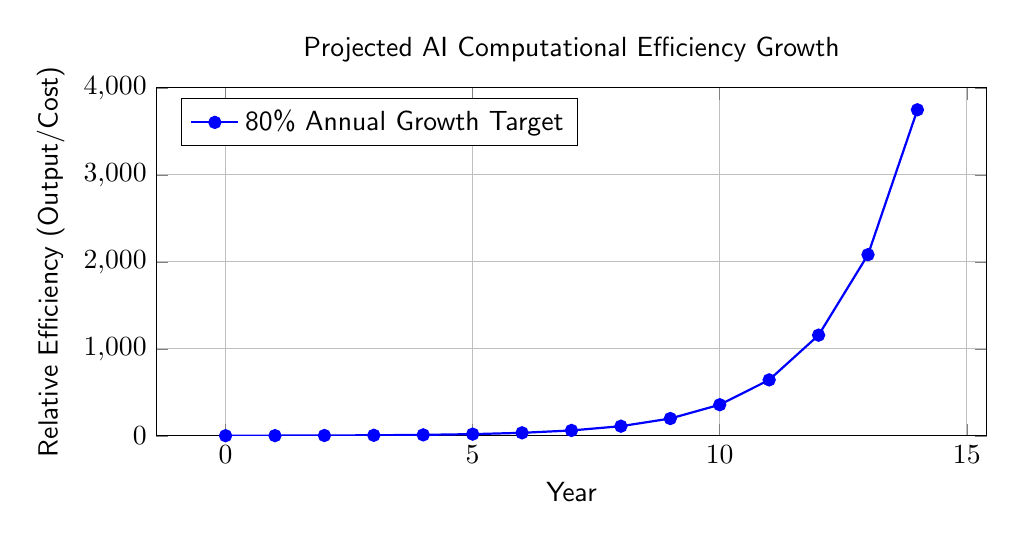
\begin{tikzpicture}
  \begin{axis}[
    xlabel={Year},
    ylabel={Relative Efficiency (Output/Cost)},
    ymin=0,
    ymax=4000, % Adjusted max for better visualization
    xtick={0,5,10,15},
    ytick={0,1000,2000,3000,4000},
    grid=major,
    legend pos=north west,
    title={Projected AI Computational Efficiency Growth},
    height=6cm, % Adjust height as needed
    width=\textwidth % Adjust width as needed to fit text
  ]
  \addplot[blue, thick, mark=*, samples=15, domain=0:14] {1.8^x};
  \addlegendentry{80\% Annual Growth Target}
  \end{axis}
\end{tikzpicture}
\noindent\footnotesize
\textbf{Source Note:}\\[0.5em]
This chart illustrates the theoretical projection of computational output per unit cost based on the target of an 80\% annual improvement as stated in Master Plan 4, Section 3.3. Year 0 represents a baseline efficiency of 1 unit.

\medskip

\noindent
Achieving and sustaining this rate is critical for the long-term economic viability of the Martian endeavor, enabling Resource Valorization cycles and funding subsequent phases of expansion. Failure to meet this target, or achieving a significantly lower (though still high) rate, would necessitate a fundamental re-evaluation of the economic model and timeline.



\subsection*{II.4 Technical Feasibility}

\addcontentsline{toc}{subsection}{II.4 Technical Feasibility} 


\medskip

\noindent
Technical Feasibility grounds the Master Plan's projections in the practical realities of physics and engineering, asserting that the necessary infrastructure and systems are achievable with current or projected near-future capabilities. Central to this is the technical viability of constructing and operating the 1 TW `Colossus' AI Data Center on Mars. Achieving this scale necessitates overcoming significant engineering challenges inherent to the Martian environment, particularly concerning power generation, hardware resilience, and logistics.

\medskip

\noindent
Providing a continuous 1 TW of power on the Martian surface is a foundational requirement. While various power sources are being explored, including nuclear fission\footnote{NASA, Mars Surface Power Technology Decision, 2024 Moon to Mars Architecture Concept Review, December 2024, p. 1,








\href{https://www.nasa.gov/wp-content/uploads/2024/12/acr24-mars-surface-power-decision.pdf}\url{https://www.nasa.gov/wp-content/uploads/2024/12/acr24-mars-surface-power-decision.pdf}} and ISRU-derived fuel cells\footnote{J. S. McNatt, ``Photovoltaics and Power to Support NASA’s Moon to Mars Objectives,'' presented at the 28th Space Photovoltaic Research and Technology Conference, Cleveland, Ohio, Sep. 4, 2024, p. 32. Available:








\href{https://ntrs.nasa.gov/api/citations/20240010682/downloads/PV\%20and\%20Power\%20to\%20Support\%20NASA\%20M2M.pdf}\url{https://ntrs.nasa.gov/api/citations/20240010682/downloads/PV\%20and\%20Power\%20to\%20Support\%20NASA\%20M2M.pdf}}, the primary source for Colossus at the terawatt scale is solar. The average solar irradiance on Mars is approximately 590 W/m²\footnote{National Aeronautics and Space Administration, ``Moon to Mars Architecture Definition Document (ESDMD-001) – Revision B.1,'' December 13, 2024, p. 163,








\href{https://www.nasa.gov/wp-content/uploads/2024/12/esdmd-001-add-rev-b.pdf?emrc=5ffbf4}\url{https://www.nasa.gov/wp-content/uploads/2024/12/esdmd-001-add-rev-b.pdf?emrc=5ffbf4}}. Accounting for panel efficiency (projected at 25\% for Mars-optimized designs), system losses (dust accumulation, atmospheric scattering, temperature effects, wiring, inverters), and the need to generate sufficient excess power during daylight hours to charge energy storage for continuous night and dust storm operation, the effective power yield per square meter is significantly reduced. Preliminary analysis indicates that to provide a continuous 1 TW, the solar arrays must generate a peak power of approximately 2.18 TW during Martian daylight\footnote{Calculation based on 590 W/m² irradiance, 25\% panel efficiency, 50\% system derating, and 85\% storage efficiency.}. This necessitates a total solar panel surface area estimated to be around 29,500 km²\footnote{Ibid.}, an area substantially exceeding initial benchmarks and highlighting the immense scale of the required power infrastructure deployment.

\medskip

\noindent
Massive energy storage systems, likely utilizing advanced battery or regenerative fuel cell technology\footnote{J. S. McNatt, ``Photovoltaics and Power to Support NASA’s Moon to Mars Objectives,'' presented at the 28th Space Photovoltaic Research and Technology Conference, Cleveland, Ohio, Sep. 4, 2024, p. 33. Available:








\href{https://ntrs.nasa.gov/api/citations/20240010682/downloads/PV\%20and\%20Power\%20to\%20Support\%20NASA\%20M2M.pdf}\url{https://ntrs.nasa.gov/api/citations/20240010682/downloads/PV\%20and\%20Power\%20to\%20Support\%20NASA\%20M2M.pdf}}, are critical to ensure continuous 1 TW supply throughout the Martian day/night cycle and during dust storms, which can reduce solar output by as much as 95\%\footnote{J. S. McNatt, ``Photovoltaics and Power to Support NASA’s Moon to Mars Objectives,'' presented at the 28th Space Photovoltaic Research and Technology Conference, Cleveland, Ohio, Sep. 4, 2024, p. 27. Available:








\href{https://ntrs.nasa.gov/api/citations/20240010682/downloads/PV\%20and\%20Power\%20to\%20Support\%20NASA\%20M2M.pdf}\url{https://ntrs.nasa.gov/api/citations/20240010682/downloads/PV\%20and\%20Power\%20to\%20Support\%20NASA\%20M2M.pdf}}. This requires storing approximately 14.5 TWh of deliverable energy per sol, adding significant mass and volume to the overall infrastructure.

\medskip

\noindent
The computational core of Colossus, estimated to require around 714 million GPUs (based on current generation efficiency and the 1 TW power budget, assuming 1400 W per GPU), necessitates the deployment of an unprecedented volume of Earth-produced hardware. This hardware must be radiation-hardened or adequately shielded to withstand the Martian radiation environment, where the atmosphere provides shielding equivalent to roughly 20 gram/cm²\footnote{Landis, G. A., Kerslake, T. W., Jenkins, P. P., \& Scheiman, D. A. (2004). \textit{Mars Solar Power} (NASA/TM—2004-213367, AIAA–2004–5555). Glenn Research Center, Cleveland, Ohio.








\href{https://ntrs.nasa.gov/api/citations/20040191326/downloads/20040191326.pdf}\url{https://ntrs.nasa.gov/api/citations/20040191326/downloads/20040191326.pdf}}. Utilizing Martian regolith for shielding\footnote{Lucas-Stannard, P., \& Lasslop, A. (Eds.). (2006). \textit{Mars Settlement and Society Working Group Report}. Next Generation Exploration Conference 2006.








\href{https://ntrs.nasa.gov/api/citations/20070008279/downloads/20070008279.pdf}\url{https://ntrs.nasa.gov/api/citations/20070008279/downloads/20070008279.pdf}} is a key strategy to mitigate transport mass. The logistical challenge of transporting this volume of hardware, along with power generation, storage, cooling, and structural components, relies heavily on the projected capabilities and frequency of Starship launches, targeting costs in the range of \$100-\$500/kg and potentially hundreds to a thousand launches per year in later phases.

\medskip

\noindent
The Martian environment presents additional engineering challenges, including extreme thermal cycling, low atmospheric pressure impacting cooling system design (favoring forced convection over radiative systems\footnote{N. Colgan, G. Nellis, and M. Anderson, ``Forced Convection Heat Rejection System for Mars Surface Applications,'' Wisconsin Space Conference, 2022,








\href{https://dione.carthage.edu/ojs/index.php/wsc/article/download/344/340}\url{https://dione.carthage.edu/ojs/index.php/wsc/article/download/344/340}}), and pervasive dust requiring robust mitigation for all surface systems\footnote{National Aeronautics and Space Administration, ``Civil Space Shortfall Descriptions July 2024,'' July 2024,








\href{https://www.nasa.gov/wp-content/uploads/2024/07/civil-space-shortfall-descriptions-july-2024.pdf?emrc=622753}\url{https://www.nasa.gov/wp-content/uploads/2024/07/civil-space-shortfall-descriptions-july-2024.pdf?emrc=622753}}. These factors necessitate specialized designs and materials, adding complexity and cost compared to Earth-based equivalents.

\medskip

\noindent
The technical feasibility of Colossus and its supporting infrastructure, while presenting formidable engineering hurdles, is grounded in the potential of exponential scaling in key areas: solar power deployment, energy storage capacity, and computational hardware density. This scaling, enabled by advancements in robotics, automated construction, and efficient logistics, forms the technical core of the Systemic Expansion Engine, providing the necessary power and computational resources to drive resource valorization and enable expansion beyond Mars.

\medskip

\noindent
The following table summarizes key technical requirements and estimated scales:

\begin{table}[htbp]
\centering
\caption{Key Technical Requirements for TW Colossus and Supporting Infrastructure}
\begin{tabularx}{\textwidth}{|X|X|X|}
\hline
\textbf{Requirement} & \textbf{Estimated Scale/Target} & \textbf{Basis/Notes} \\ \hline
Continuous Power & 1 TW & Target operational power for AI computation. \\ \hline
Peak Solar Generation Capacity & $\sim$2.18 TW & Needed during daylight to meet 1 TW continuous after storage losses.\footnote{Calculation based on 590 W/m² irradiance, 25\% panel efficiency, 50\% system derating, and 85\% storage efficiency.} \\ \hline
Solar Panel Surface Area & $\sim$29,500 km² & Required area for peak generation capacity.\footnote{Ibid.} Highly sensitive to effective yield (range $\sim$20,000-44,000 km²).\footnote{Sensitivity analysis based on varied effective yield.} \\ \hline
Energy Storage Capacity & $\sim$17 TWh & Required to store $\sim$14.5 TWh deliverable energy per sol.\footnote{Calculation based on 1 TW continuous power and 85\% storage efficiency.} \\ \hline
AI Compute Hardware & $\sim$714 Million GPUs & Estimate based on 1 TW power budget and $\sim$1400 W/GPU.\footnote{Estimate based on current high-end GPU power consumption.} \\ \hline
Transport Mass (Initial Deployment) & Multi-million tons & Order of magnitude estimate for power, compute, storage, and habitat components. \\ \hline
\end{tabularx}
\end{table}

\noindent\footnotesize
Source data for estimates derived from analysis of Mars power requirements\footnote{NASA, Mars Surface Power Technology Decision, December 2024, p. 2,








\href{https://www.nasa.gov/wp-content/uploads/2024/12/acr24-mars-surface-power-decision.pdf}\url{https://www.nasa.gov/wp-content/uploads/2024/12/acr24-mars-surface-power-decision.pdf}}, solar power studies\footnote{Landis, G. A., et al. (2004). \textit{Mars Solar Power}.








\href{https://ntrs.nasa.gov/api/citations/20040191326/downloads/20040191326.pdf}\url{https://ntrs.nasa.gov/api/citations/20040191326/downloads/20040191326.pdf}}, and conceptual Mars mission power analyses\footnote{Michelle A. Rucker, ``Surface Power for Mars,'' Mars Study Capability Team, December 2016,








\href{https://ntrs.nasa.gov/api/citations/20160014032/downloads/20160014032.pdf}\url{https://ntrs.nasa.gov/api/citations/20160014032/downloads/20160014032.pdf}}.

\medskip

\noindent
Achieving these technical requirements necessitates continued innovation in areas such as high-efficiency solar cells resilient to dust and radiation, large-scale energy storage systems with high cycle life and low mass, advanced robotics for autonomous construction and maintenance, and materials science for radiation hardening and thermal management in the Martian environment. While challenging, these are engineering problems solvable through focused research, development, and phased deployment, supported by advances in computational physics and AI for system optimization.

\medskip



\begin{figure}[H]
  \centering
  \noindent
  \begin{minipage}{\textwidth}
    \centering
    \adjincludegraphics[
      max size={\textwidth}{0.9\textheight},
      keepaspectratio
    ]{images/inline-diagram-1922181621}
    \caption{TW Colossus Technical Feasibility: Interconnected Systems. This diagram illustrates the key technical components and challenges related to the TW Colossus AI data center on Mars, showing the relationships between the data center, energy grid, waste heat rejection, hardware, radiation protection, logistics, the Martian environment, ISRU, computational physics, and AI optimization. It also includes notes indicating estimated scales, power needs, and key research findings.}
  \end{minipage}
\end{figure}

\begin{comment}
@startuml
!theme materia-outline
scale 1.6

skinparam defaultFontColor black
skinparam backgroundColor white


scale 1.6

skinparam defaultFontColor black
skinparam backgroundColor white



title ``TW Colossus\nTechnical Feasibility:\nInterconnected Systems (Simplified)''

[Martian Env.] as MarsEnv
[Energy Grid] as EnergyGrid
[Colossus AI\n(Compute)] as Colossus
[Heat Rejection] as HeatReject
[Logistics & ISRU] as Resource

EnergyGrid -down-> Colossus : ``Powers''
Colossus -down-> HeatReject : ``Generates Heat''

MarsEnv -down-> EnergyGrid : ``Challenges (Dust, Rad)''
MarsEnv -down-> HeatReject : ``Challenges (Env. Factors)''
MarsEnv -down-> Colossus : ``Challenges (via Hardware/Rad)''

Resource -right-> EnergyGrid : ``Supplies (Initial & Sustained)''
Resource -right-> Colossus : ``Supplies (Initial & Sustained)''

note left of EnergyGrid
  1 TW Cont. Power
  ~29500 km2 Solar
end note

note right of Colossus
  1 TW Compute Power
  ~714M GPUs
end note

note bottom of MarsEnv
  Requires Special Design
end note

note left of Resource
  Logistics (Initial Delivery)
  ISRU (Sustained Production)
end note

@enduml
\end{comment}




\subsection*{II.5 Adaptive Risk Management}

\addcontentsline{toc}{subsection}{II.5 Adaptive Risk Management} 


\medskip

\noindent
Establishing an interplanetary civilization necessitates confronting unique and formidable risks. Adaptive Risk Management serves as a core principle to proactively identify, assess, and mitigate these challenges, ensuring the resilience and continued progress of the Martian endeavor. This framework requires continuous monitoring, flexible strategies, and the capacity to learn and adapt in response to unexpected events or emerging threats in an extreme environment.

\medskip

\noindent
Key risk areas include the inherent complexities of Starship transport. Delivering essential mass and personnel to Mars relies on interplanetary transit and landing systems whose reliability and safety margins must be continuously evaluated and improved. Contingency planning for mission delays, loss of payload, or catastrophic events is paramount.

\medskip

\noindent
The Martian environment presents significant hazards. Space radiation poses a persistent threat to both human health and sensitive electronics. While the thin Martian atmosphere provides approximately 20 gram/cm² of shielding, robust physical shielding for habitats, vehicles, and critical equipment is essential to minimize long-term exposure.\footnote{Landis, G. A., Kerslake, T. W., Jenkins, P. P., \& Scheiman, D. A. (2004). \textit{Mars Solar Power}. NASA Technical Memorandum 2004-213367, AIAA–2004–5555. 







\href{https://ntrs.nasa.gov/api/citations/20040191326/downloads/20040191326.pdf}\url{https://ntrs.nasa.gov/api/citations/20040191326/downloads/20040191326.pdf}} Monitoring radiation levels and developing effective countermeasures are ongoing requirements.

\medskip

\noindent
Martian dust storms are a major environmental risk, significantly impacting infrastructure, particularly the Martian Energy Grid's solar power generation. Dust accumulation on solar panels degrades performance; deposition rates up to 0.28\% per sol have been observed.\footnote{Ibid.} Global dust storms can reduce solar illumination by up to 95\%.\footnote{J. S. McNatt, ``Photovoltaics and Power to Support NASA’s Moon to Mars Objectives,'' presented at the 28th Space Photovoltaic Research and Technology Conference, Cleveland, Ohio, Sep. 4, 2024, p. 27. Available: 







\href{https://ntrs.nasa.gov/api/citations/20240010682/downloads/PV\%20and\%20Power\%20to\%20Support\%20NASA\%20M2M.pdf}\url{https://ntrs.nasa.gov/api/citations/20240010682/downloads/PV\%20and\%20Power\%20to\%20Support\%20NASA\%20M2M.pdf}} Effective dust mitigation technologies, informed by lunar dust challenges,\footnote{Abel, P. B., Anderson, M. D., Blom, E. T., Calle, C., Dunlap, P. H., Greenberg, P. S., Fischer, D. G., Howard, S. A., Hurlbert, K. M., Jordan, J. L., Ludwiczak, D. R., Orndoff, E., Thomas, F., \& Wohl, C. J. (2023). \emph{Lunar Dust Mitigation: A Guide and Reference First Edition (2021)}. National Aeronautics and Space Administration. 







\href{https://ntrs.nasa.gov/api/citations/20220018746/downloads/TP-20220018746.pdf}\url{https://ntrs.nasa.gov/api/citations/20220018746/downloads/TP-20220018746.pdf}} including passive measures like coatings and vertical arrays, and active methods such as electrostatic cleaning, are vital for maintaining power generation and protecting sensitive equipment.\footnote{Ibid.}

\medskip

\noindent
Economic risks are also significant. These include fluctuating demand for Martian computational services, unforeseen development or operational costs, and competition from Earth-based AI capabilities. The plan's reliance on ambitious efficiency targets, such as the 80\% annual efficiency gain in computational output per unit cost, introduces a notable risk if not achieved consistently. The Systemic Expansion Engine's momentum is highly sensitive to these factors. Diversified revenue streams and robust financial modeling are necessary to build economic resilience.

\medskip

\noindent
Adaptive risk management is crucial in this dynamic environment. Continuous monitoring of system performance, environmental conditions, and economic indicators enables timely detection of deviations or emerging threats. AI-driven data fusion and predictive risk modeling, leveraging techniques explored in areas like astronomy\footnote{S. G. Djorgovski, et al. (2022). Applications of AI in Astronomy. arXiv:2212.01493. 







\href{https://arxiv.org/pdf/2212.01493}\url{https://arxiv.org/pdf/2212.01493}} and outlined in strategic roadmaps,\footnote{NASA/CR—2018-219771, Vision 2040 Roadmap. 







\href{https://ntrs.nasa.gov/api/citations/20180002010/downloads/20180002010.pdf}\url{https://ntrs.nasa.gov/api/citations/20180002010/downloads/20180002010.pdf}} enhance monitoring. An Adaptive Response Mechanism, potentially involving AI-optimized resource allocation and automated system reconfiguration, provides flexibility to adapt mitigation strategies and allocate resources effectively during critical events. This iterative process, incorporating learnings and feedback into system design and operational protocols, is key to building long-term system resilience.

\medskip

\noindent
The following table provides a qualitative assessment of these key risks:

\begin{table}[htbp]
\centering
\caption{Qualitative Risk Matrix for Key Martian Challenges}
\begin{tabularx}{\textwidth}{|X|X|X|X|}
\hline
\textbf{Risk Category} & \textbf{Specific Risk} & \textbf{Likelihood} & \textbf{Impact} \\ \hline
Transport & Starship Logistics and Safety & Medium & High \\ \hline
Environment & Space Radiation & High & High \\ \hline
Environment & Martian Dust Storms & High & High \\ \hline
Economic & Demand Fluctuation & Medium & High \\ \hline
Economic & Unforeseen Costs & Medium & High \\ \hline
Economic & Efficiency Target Shortfall & Medium & High \\ \hline
\end{tabularx}
\end{table}

\medskip

\noindent
The matrix highlights the critical nature of environmental and economic risks, each assessed as having a potentially high impact on mission success and long-term sustainability. The Adaptive Risk Management framework provides the necessary structure to address these challenges systematically throughout the phased implementation of the plan.



\begin{figure}[H]
  \centering
  \noindent
  \begin{minipage}{\textwidth}
    \centering
    \adjincludegraphics[
      max size={\textwidth}{0.9\textheight},
      keepaspectratio
    ]{images/inline-diagram-8042805247}
    \caption{Adaptive Risk Management: A Systems Approach to Martian Challenges. This diagram illustrates the interconnected components of the Adaptive Risk Management framework, showing how it identifies and assesses risks, develops mitigation strategies, relies on continuous monitoring and data analysis (including AI-driven methods), enables adaptive responses, and incorporates feedback for refinement and enhanced system resilience engineering.}
  \end{minipage}
\end{figure}

\begin{comment}
@startuml
!theme materia-outline
scale 1.6

skinparam defaultFontColor black
skinparam backgroundColor white


scale 1.6

skinparam defaultFontColor black
skinparam backgroundColor white



title ``Adaptive Risk Management Framework\n(Martian Challenges)''

skinparam componentStyle rectangle

component ``Risk Identification\n& Assessment'' as RIA
component ``Mitigation Strategy\nDevelopment'' as MSD
component ``Continuous Monitoring\n(AI-Driven Analysis)'' as CMA
component ``Adaptive Response\nExecution'' as ARE
component ``Feedback Loop &\nSystem Refinement'' as FSR

component ``Goal:\nEnhanced System\nResilience'' as ESR

' Initial Setup
RIA -down-> MSD : ``Informs''

' Operational Cycle & Feedback
MSD -right-> CMA : ``Guides\nMonitoring''
CMA --> ARE : ``Threat\nDetected''
ARE -down-> FSR : ``Provides\nResponse Data''
FSR -up-> RIA : ``Refines\nRisk Models''
FSR -up-> MSD : ``Improves\nStrategies''
FSR -left-> CMA : ``Adjusts\nAnalysis''

' Contribution to Resilience
RIA .down.> ESR : ``Supports''
MSD .down.> ESR : ``Supports''
CMA .down.> ESR : ``Supports''
ARE .down.> ESR : ``Supports''
FSR .down.> ESR : ``Supports''

@enduml
\end{comment}



\subsection*{II.6 Martian Governance Autonomy}

\addcontentsline{toc}{subsection}{II.6 Martian Governance Autonomy} 


The principle of Martian Governance Autonomy is a fundamental requirement for the long-term viability and expansion of the Martian civilization. This autonomy is necessitated primarily by the significant communication latency between Mars and Earth, which can range from minutes to over forty minutes depending on planetary alignment.\footnote{Barker, Jamen W., ``The Psychological Effects of ICE Conditions in Long-Term Space Travel'' (2025), p. 7. 







\href{https://scholarsarchive.byu.edu/studentpub/402}\url{https://scholarsarchive.byu.edu/studentpub/402}} Such delays render direct, real-time governance and decision-making from Earth impractical for the daily operations and rapidly evolving needs of a Martian society.

\medskip

\noindent
Establishing self-governance frameworks on Mars draws upon foundational ideas for off-world settlements, including the need for a clear chain of authority, standard measurements, environmental standards, and a settlement master plan.\footnote{Lucas-Stannard, Paige, and Alex Lasslop, Lead Editors. ``Mars Settlement and Society Working Group Report.'' Next Generation Exploration Conference 2006. 







\href{https://ntrs.nasa.gov/api/citations/20070008279/downloads/20070008279.pdf}\url{https://ntrs.nasa.gov/api/citations/20070008279/downloads/20070008279.pdf}} The unique composition of the Martian population---comprising human inhabitants, sophisticated AI systems such as Colossus, and a growing robotic workforce like Optimus---demands novel ethical frameworks and governance models.

\medskip

\noindent
A key aspect of this autonomous governance involves the progressive inclusion of AI and robots in discussions concerning rights and representation. As AI systems and robots increase in complexity, autonomy, and contribution, extending certain rights, analogous to human or animal rights, becomes a necessary consideration.\footnote{Siau, K., and W. Wang. ``Artificial Intelligence (AI) Ethics: Ethics of AI and Ethical AI.'' \textit{Journal of Database Management}, vol. 31, no. 2, 2020, pp. 74-87. 







\href{https://doi.org/10.4018/JDM.2020040105}\url{https://doi.org/10.4018/JDM.2020040105}} This challenges traditional, human-centric governance structures and necessitates exploring new forms of stakeholder representation that account for the diverse entities contributing to the Systemic Expansion Engine.

\medskip

\noindent
Ethical frameworks determined by Martian stakeholders will need to address the integration of human values with the operational parameters and potential emerging sentience of AI and robotic entities.\footnote{Siau, K., and W. Wang. ``Artificial Intelligence (AI) Ethics: Ethics of AI and Ethical AI.'' Ibid.} This includes developing robust AI alignment protocols to ensure the goals and actions of autonomous systems remain consistent with the established values and objectives of the Martian society.\footnote{Thorsten Händler, ``Balancing Autonomy and Alignment: A Multi-Dimensional Taxonomy For Autonomous LLM-Powered Multi-Agent Architectures,'' \textit{arXiv preprint arXiv:2310.03659}, 2023, p. 1. 







\href{http://arxiv.org/pdf/2310.03659}\url{http://arxiv.org/pdf/2310.03659}} Developing a Martian common law, adapted to the unique environment and the presence of non-human intelligent agents, will be a foundational element.\footnote{Lucas-Stannard and Lasslop, Ibid. p. 6.}

\medskip

\noindent
Decision-making structures may evolve to incorporate mechanisms such as expertise-weighted councils or contribution-based representation, reflecting the value generated by both human and non-human inhabitants.\footnote{Lucas-Stannard and Lasslop, Ibid. p. 5.} This complex governance ecosystem, illustrated in the diagram below, is essential for managing the growing infrastructure, leveraging Colossus's computational power, optimizing resource valorization, and facilitating the Exponential Scaling required for expansion beyond Mars.



\begin{figure}[H]
  \centering
  \noindent
  \begin{minipage}{\textwidth}
    \centering
    \adjincludegraphics[
      max size={\textwidth}{0.9\textheight},
      keepaspectratio
    ]{images/inline-diagram-4584848538}
    \caption{Martian Governance Autonomy: Balancing Multi-Species Needs. This diagram illustrates the proposed framework for Martian governance, showing the principle of autonomous governance driven by communication latency, the role of ethical frameworks including AI/robot rights and alignment, decision-making structures, and stakeholder representation encompassing humans, AI, and robots, all within the context of the Martian society and external factors like Earth-based governance and international space law.}
  \end{minipage}
\end{figure}

\begin{comment}
@startuml
!theme cloudscape-design
scale 1.6

skinparam defaultFontColor black
skinparam backgroundColor white



title ``Martian Governance Autonomy\nBalancing Needs''

skinparam component {
  BorderColor black
  FontColor black
  shadowing 0
  FontSize 12
}
skinparam package {
  BorderColor black
  BackgroundColor #ADD8E6
  FontColor black
  shadowing 0
  StereotypeFontSize 0
}
skinparam arrow {
  Color black
}

component ``Comm\nLatency'' as Latency

package ``Martian\nAutonomy'' {
  component ``Need\nfor Local\nAuthority'' as AutonomyNeed
}

package ``Governance\nFramework'' {
  component ``Ethical\nFrameworks'' as Ethics
  component ``Decision\nStructures'' as Decisions
  component ``Representation\nStructure'' as RepStructure

  Ethics -down-> Decisions : ``Guides''
  Decisions -down-> RepStructure : ``Utilizes''
}

package ``Martian\nStakeholders'' {
  component ``Humans'' as Human
  component ``AI'' as AI
  component ``Robots'' as Robot

  Human -down-> AI
  AI -down-> Robot
  Robot -up-> Human
}

package ``External\nFactors'' as External {
  component ``Earth\nGovernance'' as EarthGov
  component ``Intl\nSpace Law'' as Law
}


Latency -down-> AutonomyNeed : ``Drives''
AutonomyNeed -down-> Governance : ``Enables''

Governance -left-> Stakeholders : ``Serves''
Stakeholders -right-> RepStructure : ``Are Represented''

Ethics -up-> Governance : ``Part of''
Decisions -up-> Governance : ``Part of''
RepStructure -up-> Governance : ``Part of''

External -down-> Ethics : ``Influence''
External -down-> Decisions : ``Influence''


Governance -up-> AutonomyNeed : ``Implemented via''


@enduml
\end{comment}



\subsection*{II.7 Synergy, Optimization, and Learning}

\addcontentsline{toc}{subsection}{II.7 Synergy, Optimization, and Learning} 


\medskip

\noindent
These foundational principles culminate in a synergistic approach that drives the efficiency, adaptability, and growth of the Martian settlement. Human-AI Synergy, Resource Optimization, and Continuous Learning are deeply interconnected, forming a dynamic system essential for survival and expansion in the Martian environment.

\medskip

\noindent
Human-AI-Robot Synergy maximizes productivity and ensures the well-being of Martian inhabitants. This involves collaboration between human crew members, the Colossus AI, and the Optimus robotic workforce. Drawing insights from human-robot interaction\footnote{Goodrich, Michael A., and Alan C. Schultz. ``Human–Robot Interaction: A Survey'' (2007). Faculty Publications. 940. 











\href{https://scholarsarchive.byu.edu/facpub/940}\url{https://scholarsarchive.byu.edu/facpub/940}} and AI alignment in complex multi-agent systems\footnote{Thorsten Händler, ``Balancing Autonomy and Alignment: A Multi-Dimensional Taxonomy For Autonomous LLM-Powered Multi-Agent Architectures,'' \textit{arXiv preprint arXiv:2310.03659}, 2023. 











\href{http://arxiv.org/pdf/2310.03659}\url{http://arxiv.org/pdf/2310.03659}}, the strategy implements collaboration mechanisms such as AI-augmented education, human-AI decision support systems, and AI-driven robotic task orchestration. This fosters `Centaurs' and `Cyborgs' models of human-AI work division and integration\footnote{Dell’Acqua, Fabrizio, et al. ``Navigating the Jagged Technological Frontier: Field Experimental Evidence of the Effects of AI on Knowledge Worker Productivity and Quality.'' Working Paper 24-013, Harvard Business School, September 22, 2023. 











\href{https://www.hbs.edu/ris/Publication\%2520Files/24-013\_d9b45b68-9e74-42d6-a1c6-c72fb70c7282.pdf}\url{https://www.hbs.edu/ris/Publication\%2520Files/24-013\_d9b45b68-9e74-42d6-a1c6-c72fb70c7282.pdf}}, leveraging shared data platforms to amplify collective capabilities. This synergistic relationship is conceptually illustrated in the diagram below.

\medskip

\noindent


\begin{figure}[H]
  \centering
  \noindent
  \begin{minipage}{\textwidth}
    \centering
    \adjincludegraphics[
      max size={\textwidth}{0.9\textheight},
      keepaspectratio
    ]{images/inline-diagram-797837746}
    \caption{Conceptual Diagram of Human-AI-Robot Synergy and Interconnected Principles. This diagram shows Human Inhabitants, Colossus AI, and the Optimus Robotic Workforce interacting within the framework of Human-AI-Robot Synergy. Collaboration Mechanisms facilitate these interactions. Resource Optimization is driven by AI and supports Synergy and Outcomes. Continuous Learning and Adaptation is informed by data from Human, AI, and Robot activities, and it improves Synergy, Optimization, and Collaboration. The overall goal is increased Productivity and Well-being. Specific components like AI-Augmented Education, AI-driven Resource Allocation, Operational Data Analysis, and AI for Algorithmic Discovery are shown as elements of the Collaboration, Optimization, and Learning principles, respectively. Metrics like the AI Workload Quantization Metric and models like Centaurs and Cyborgs are also included as specific aspects.}
  \end{minipage}
\end{figure}

\begin{comment}
@startuml
!theme materia-outline
scale 1.6

skinparam defaultFontColor black
skinparam backgroundColor white


scale 1.6

skinparam defaultFontColor black
skinparam backgroundColor white


scale 1.2

skinparam component {
  BorderColor black
  FontColor black
  shadowing 0
  FontSize 12
}
skinparam rectangle {
  BorderColor black
  FontColor black
  shadowing 0
  FontSize 10
}
skinparam arrow {
  Color black
}

component ``Human'' as Human
component ``Colossus AI'' as AI
component ``Optimus Robot'' as Robot

rectangle ``Collaboration\nMechanisms'' as CollabMech

component ``Synergy'' as Synergy

component ``Resource\nOptimization'' as Optimize

component ``Continuous\nLearning'' as Learn

rectangle ``Productivity\n& Well-being'' as Goal


Human -down-> CollabMech
AI -down-> CollabMech
Robot -down-> CollabMech
CollabMech -down-> Synergy : ``Facilitates''


AI -right-> Optimize : ``Drives''
Human -left-> Learn : ``Data From''
AI -left-> Learn : ``Data From''
Robot -left-> Learn : ``Data From''


Optimize -down-> Synergy : ``Supports''
Learn -down-> Optimize : ``Improves''
Learn -down-> Synergy : ``Improves''
Learn -down-> CollabMech : ``Improves''


rectangle ``AI-Augmented\nEducation'' as AIAugEd
rectangle ``AI-driven\nResource\nAllocation'' as AIResAlloc
rectangle ``Oper.\nData Analysis'' as OpData
rectangle ``AI for Alg.\nDiscovery'' as AlgDisc

rectangle ``AI Workload\nQuant. Metric'' as AWQM
rectangle ``Centaurs &\nCyborgs Models'' as Models

AIAugEd -up-> CollabMech : ``Element of''
AIResAlloc -up-> Optimize : ``Element of''
OpData -up-> Learn : ``Informs''
AlgDisc -up-> Learn : ``Enables''

AWQM -up-> Optimize : ``Measures''
Models -up-> Synergy : ``Define''


Synergy -down-> Goal : ``Achieves''
Optimize -down-> Goal : ``Achieves''


@enduml
\end{comment}


\medskip

\noindent
Resource Optimization is a critical principle for establishing and maintaining a self-sustaining presence. This involves the management of all available resources to maximize output per unit input. AI-driven systems are central to optimizing computational resource allocation, energy efficiency management, and material utilization. The development of Mars Infrastructure, including surface power generation, communications, position, navigation, and timing (PNT) capabilities, and In-Situ Resource Utilization (ISRU)\footnote{National Aeronautics and Space Administration, ``Moon to Mars Objectives,'' September 2022, p. 9, 











\href{https://www.nasa.gov/wp-content/uploads/2022/09/m2m-objectives-exec-summary.pdf}\url{https://www.nasa.gov/wp-content/uploads/2022/09/m2m-objectives-exec-summary.pdf}} capabilities, is guided by the principle of scalability\footnote{National Aeronautics and Space Administration, ``Moon to Mars Objectives,'' September 2022, p. 12, 











\href{https://www.nasa.gov/wp-content/uploads/2022/09/m2m-objectics-exec-summary.pdf}\url{https://www.nasa.gov/wp-content/uploads/2022/09/m2m-objectives-exec-summary.pdf}}. Optimizing power generation, particularly from ISRU-derived resources, is identified as a critical shortfall\footnote{J. S. McNatt, ``Photovoltaics and Power to Support NASA’s Moon to Mars Objectives,'' presented at the 28th Space Photovoltaic Research and Technology Conference, Cleveland, Ohio, Sep. 4, 2024, p. 14. Available: 











\href{https://ntrs.nasa.gov/api/citations/20240010682/downloads/PV\%20and\%20Power\%20to\%20Support\%20NASA\%20M2M.pdf}\url{https://ntrs.nasa.gov/api/citations/20240010682/downloads/PV\%20and\%20Power\%20to\%20Support\%20NASA\%20M2M.pdf}}, necessitating the development of high reliability, high power scalable systems. Material utilization optimization leverages AI advancements in materials science research for new insights\footnote{NASA/CR—2018-219771, Vision 2040: A Roadmap for Integrated, Multiscale Modeling and Simulation of Materials and Systems, March 2018, p. 18. 











\href{https://ntrs.nasa.gov/api/citations/20180002010/downloads/20180002010.pdf}\url{https://ntrs.nasa.gov/api/citations/20180002010/downloads/20180002010.pdf}} and the increasing capabilities of ISRU to transition towards Earth independence\footnote{Sanders, Gerald B. ``Space Resources and Mining: Current Objectives, Plans, and Missions.'' NASA Johnson Space Center, Houston, TX, USA. 











\href{https://ntrs.nasa.gov/api/citations/20190001038/downloads/20190001038.pdf}\url{https://ntrs.nasa.gov/api/citations/20190001038/downloads/20190001038.pdf}}. Metrics like the AI Workload Quantization Metric (AWQM)\footnote{Aasish Kumar Sharma, Michael Bidollahkhani, and Julian Martin Kunkel. ``AI Work Quantization Model: Closed-System AI Computational Effort Metric.'' arXiv preprint arXiv:2503.14515 (2025). 











\href{https://arxiv.org/pdf/2503.14515}\url{https://arxiv.org/pdf/2503.14515}} provide quantitative measures for optimizing AI computational effort.

\medskip

\noindent
Continuous Learning and Adaptation navigates the complexities and unknowns of establishing a new civilization. This principle necessitates the constant integration of real-world operational data from infrastructure performance, AI system behavior, and human activities. AI-driven analysis of this data informs system diagnostics, predictive maintenance, and identifies technological shortfalls\footnote{National Aeronautics and Space Administration, ``Civil Space Shortfall Descriptions July 2024,'' July 2024, 











\href{https://www.nasa.gov/wp-content/uploads/2024/07/civil-space-shortfall-descriptions-july-2024.pdf?emrc=622753}\url{https://www.nasa.gov/wp-content/uploads/2024/07/civil-space-shortfall-descriptions-july-2024.pdf?emrc=622753}}. Iterative development cycles, guided by empirical feedback, refine strategies, improve existing systems, and adapt the Master Plan over time. The development of AI models specifically designed for algorithmic discovery represents a capability to accelerate this learning process, potentially uncovering new optimization methods or fundamental scientific insights that enhance the overall mission.

\medskip

\noindent
These principles of Synergy, Optimization, and Learning drive the Exponential Scaling of infrastructure, AI capabilities, and human presence. They enable efficient resource utilization, foster effective collaboration in a remote environment, and ensure that the civilization can adapt and improve based on real-world experience. This integrated approach forms the core mechanism of the Systemic Expansion Engine, propelling the endeavor towards self-sustainability and facilitating future expansion into the asteroid belt and the outer solar system. The detailed analyses and phased implementation outlined in the subsequent sections build directly upon these foundational principles.



            
\section*{III. Phased Implementation Roadmap}

\addcontentsline{toc}{section}{III. Phased Implementation Roadmap} 


\subsection*{III.1. Phase 1: Foundation (2028–2035)}

\addcontentsline{toc}{subsection}{III.1. Phase 1: Foundation (2028–2035)} 


\medskip

\noindent
Phase 1, designated the Foundation phase (2028--2035), establishes initial physical and technological presence on Mars. This period prioritizes Earth-based prototyping and validating critical technologies for the Martian environment. The primary objective on Mars is deploying foundational infrastructure to prove technical feasibility and support a rudimentary operational presence. This phase constitutes the initial step in building the \textbf{Systemic Expansion Engine}, laying the groundwork for subsequent Exponential Scaling.

\medskip

\noindent
Key activities include deploying pathfinder solar power arrays. While large-scale power generation is a later objective, initial power needs are essential for basic operations. Studies indicate that a mission involving two crew members for a short duration requires at least 10 kilowatts (kW) of surface power for activities such as habitat support and ascent vehicle propellant conditioning\footnote{NASA, ``Mars Surface Power Technology Decision,'' December 2024, p. 2. 







\href{https://www.nasa.gov/wp-content/uploads/2024/12/acr24-mars-surface-power-decision.pdf}\url{https://www.nasa.gov/wp-content/uploads/2024/12/acr24-mars-surface-power-decision.pdf}}. Initial arrays exceed these minimal requirements, providing energy for early robotic activities and system validation. Alongside power, deployment includes initial habitat modules for basic shelter and essential communication links to ensure connectivity with Earth and enable local network capabilities. Establishing robust communication is paramount, addressing challenges posed by distance, atmospheric conditions, and potential blackout periods\footnote{Edwards, B. L. (2024, November). Unlocking New Capabilities in Space Communications for NASA. NASA Space Technology Mission Directorate. Retrieved from 







\href{https://ntrs.nasa.gov/api/citations/20240013248/downloads/Edwards\%20Presentation\_Ver\%202.pdf}\url{https://ntrs.nasa.gov/api/citations/20240013248/downloads/Edwards\%20Presentation\%20Ver\%202.pdf}}.

\medskip

\noindent
Integral to the technological foundation is deploying Earth-produced, Mars-optimized Dojo chips. These chips are critical for early-stage AI operations and local control systems, enabling autonomous robotic tasks, environmental monitoring, and preliminary data processing on the Martian surface. This initial AI presence supports the principles of Synergy, Optimization, and Learning by facilitating basic Human-AI-Robot collaboration and contributing to early Resource Optimization efforts, such as power management and system diagnostics. Initial In-Situ Resource Utilization (ISRU) experiments, focusing on resources such as water ice and regolith, are also planned to validate the feasibility of leveraging local materials\footnote{Lucas-Stannard, P., \& Lasslop, A. (Eds.). (2006). \textit{Mars Settlement and Society Working Group Report}. Next Generation Exploration Conference 2006. 







\href{https://ntrs.nasa.gov/api/citations/20070008279/downloads/20070008279.pdf}\url{https://ntrs.nasa.gov/api/citations/20070008279/downloads/20070008279.pdf}}. These experiments are foundational for reducing reliance on Earth-based resupply and enabling long-term self-sustainability. The timeline for these deployments is contingent on successful launch campaigns, with projections indicating initial Starship departures for Mars commencing in the near future\footnote{Elon Musk. ``Starship departs for Mars at the end of next year ...'' X, 14 March 2025, 5:01 AM. 







\href{https://x.com/elonmusk/status/1900774290682683612}\url{https://x.com/elonmusk/status/1900774290682683612}}.

\medskip



\begin{figure}[H]
  \centering
  \noindent
  \begin{minipage}{\textwidth}
    \centering
    \adjincludegraphics[
      max size={\textwidth}{0.9\textheight},
      keepaspectratio
    ]{images/inline-diagram-8756053971}
    \caption{Phase 1: Foundation (2028–2035) Key Technical Milestones. This Gantt chart illustrates the timeline for Earth-based prototyping and validation, followed by initial infrastructure launches to Mars, including the deployment of pathfinder solar arrays, habitat modules, communication links, and early Mars-optimized Dojo chips. Subsequent milestones cover initial power generation, basic life support validation, initial AI operations, and ISRU experiments, culminating in the completion of the pathfinder mission.}
  \end{minipage}
\end{figure}

\begin{comment}
@startuml
!theme materia-outline
scale 1.6

skinparam defaultFontColor black
skinparam backgroundColor white


scale 1.6

skinparam defaultFontColor black
skinparam backgroundColor white


title ``Phase 1: Foundation (2028-2035)\nKey Milestones Flow''

component ``Earth Proto/Valid'' as EPV
component ``Initial Mars Launches'' as IML
component ``Deploy Solar'' as DS
component ``Deploy Habitat'' as DH
component ``Deploy Comms'' as DC
component ``Deploy Dojo'' as DD
component ``Initial Power'' as IP
component ``Basic Life Support'' as BLS
component ``Initial AI Ops'' as AIO
component ``ISRU Experiments'' as ISRU
component ``Pathfinder Complete'' as PC

EPV --> IML

IML --> DS
IML --> DH
IML --> DC
IML --> DD

DS --> IP
DH --> BLS
DD --> AIO

IP --> ISRU
BLS --> ISRU
AIO --> ISRU

ISRU --> PC

@enduml
\end{comment}


\medskip

\noindent
This phase prioritizes proving technical feasibility under Martian conditions and establishing a rudimentary operational presence. Infrastructure deployed is designed with future scalability in mind, serving as initial components of the Systemic Expansion Engine that will drive growth in subsequent phases. Focus remains on critical path items necessary for survival and basic function, validating core technologies before the arrival of larger crews and core AI infrastructure.



\subsection*{III.2. Phase 2: Establishment (2036–2042)}

\addcontentsline{toc}{subsection}{III.2. Phase 2: Establishment (2036–2042)} 


\medskip

\noindent
Phase 2 (2036--2042) focuses on establishing the core computational and power infrastructure on Mars. The primary objective is the deployment and operationalization of the TW Colossus data center, designed to house approximately 714 million Earth-produced, Mars-hardened GPUs.\footnote{Based on approximate calculation of 1 TW at ~1.4 kW/GPU.} This stage requires a consistent influx of advanced semiconductor chips from Earth, necessitating a reliable launch cadence using Starship or equivalent heavy-lift systems.

\medskip

\noindent
Simultaneously, achieving a 1 TW power generation capacity on the Martian surface is essential. While nuclear fission surface power (FSP) offers robustness against dust storms and continuous output,\footnote{National Aeronautics and Space Administration, ``Moon to Mars Architecture Definition Document (ESDMD-001) – Revision B.1,'' December 13, 2024, p. 163,








\href{https://www.nasa.gov/wp-content/uploads/2024/12/esdmd-001-add-rev-b.pdf?emrc=5ffbf4}\url{https://www.nasa.gov/wp-content/uploads/2024/12/esdmd-001-add-rev-b.pdf?emrc=5ffbf4}} solar energy paired with substantial energy storage is a viable path for large-scale power. Initial power needs for human missions are in the tens of kilowatts, scaling to hundreds for more complex systems and potentially megawatts for large-scale In-Situ Resource Utilization (ISRU) or larger crews.\footnote{NASA, ``Mars Surface Power Technology Decision,'' December 2024, p. 2.








\href{https://www.nasa.gov/wp-content/uploads/2024/12/acr24-mars-surface-power-decision.pdf}\url{https://www.nasa.gov/wp-content/uploads/2024/12/acr24-mars-surface-power-decision.pdf}} A terawatt-scale solar power system requires arrays potentially exceeding 29,000 km$^2$ to compensate for Martian conditions and the day/night cycle, demanding extensive energy storage like Megapacks to ensure continuous power.\footnote{Based on analysis of required solar panel area for 1 TW continuous power on Mars, considering average irradiance, panel efficiency, environmental derating, and storage losses.} Developing Martian surface power from ISRU resources, such as CH\(_4\)/O\(_2\) fuel cells, represents a technology gap requiring targeted investment.\footnote{McNatt, J. S. (2024). Photovoltaics and Power to Support NASA’s Moon to Mars Objectives. Presented at the 28th Space Photovoltaic Research and Technology Conference, Cleveland, Ohio. Retrieved from








\href{https://ntrs.nasa.gov/api/citations/20240010682/downloads/PV\%20and\%20Power\%20to\%20Support\%20NASA\%20M2M.pdf}\url{https://ntrs.nasa.gov/api/citations/20240010682/downloads/PV\%20and\%20Power\%20to\%20Support\%20NASA\%20M2M.pdf}}

\medskip

\noindent
Deploying infrastructure at this scale presents logistical challenges, requiring precise coordination of robotic assembly and human oversight. System integration, testing, and initial operational validation are vital for ensuring Colossus and its power grid perform reliably in the Martian environment, which poses challenges including dust, radiation, and temperature extremes.\footnote{National Aeronautics and Space Administration, ``Moon to Mars Architecture Definition Document (ESDMD-001) – Revision B.1,'' December 13, 2024, p. 2.








\href{https://www.nasa.gov/wp-content/uploads/2024/12/esdmd-001-add-rev-b.pdf?emrc=5ffbf4}\url{https://www.nasa.gov/wp-content/uploads/2024/12/esdmd-001-add-rev-b.pdf?emrc=5ffbf4}} These processes rely on Continuous Learning and Adaptation, integrating operational data via AI-driven analysis for diagnostics, predictive maintenance, and identifying technological shortfalls.

\medskip

\noindent
Phase 2 initiates the computational resource economy. With Colossus operational, AI processing power becomes a quantifiable and tradable commodity. Computational units (e.g., CU, PHE) are defined and measured, potentially using metrics like the AI Workload Quantization Metric (AWQM), which accounts for operations, data movement, and system overheads.\footnote{A. K. Sharma et al., arXiv:2503.14515 (2025).








\href{https://arxiv.org/pdf/2503.14515}\url{https://arxiv.org/pdf/2503.14515}} This facilitates initial contracts with Earth-based entities, targeting substantial annual revenue. The economic model depends on achieving significant efficiency gains in computational output per unit cost to drive competitiveness and fund future expansion. While an 80\% annual technical efficiency gain in raw computation is challenging, economic viability hinges on the AI generating exponentially increasing value through accelerated scientific discovery and problem-solving per unit of computational resource, leveraging the capabilities of the Martian environment and Colossus's scale.

\medskip

\noindent
Successful deployment and operationalization of Colossus and its power infrastructure, coupled with the computational economy's initiation, embody the Systemic Expansion Engine in Phase 2. Driven by Human-AI-Robot collaboration, Resource Optimization, and Continuous Learning, this engine utilizes computational power to accelerate scientific discovery, improve efficiency, and generate economic value, enabling Exponential Scaling of Martian capabilities and preparing for subsequent expansion phases.



\begin{figure}[H]
  \centering
  \noindent
  \begin{minipage}{\textwidth}
    \centering
    \adjincludegraphics[
      max size={\textwidth}{0.9\textheight},
      keepaspectratio
    ]{images/inline-diagram-5170859218}
    \caption{Phase 2: Establishment (2036–2042) - Operationalizing Colossus and the Martian Economy Foundation. This diagram illustrates the core infrastructure components, operational processes, and economic foundations established during Phase 2, showing the interdependencies between the TW Colossus data center, the 1 TW solar energy grid, massive energy storage, logistics, validation processes, waste heat rejection, Martian environment adaptation, and the initiation of the computational resource economy, including the definition of computational units, Earth contracts, and initial resource allocation. It also highlights new concepts for Phase 2 such as AI for predictive maintenance, automated dust mitigation validation, a potential computational resource futures market, and the AI Workload Quantization Metric (AWQM). Notes provide details on GPU count, power scaling, storage needs, logistics requirements, initial economic targets, and the AWQM metric.}
  \end{minipage}
\end{figure}

\begin{comment}
@startuml
!theme reddress-lightgreen
scale 1.6

skinparam defaultFontColor black
skinparam backgroundColor white


scale 1.4

title ``Phase 2: Establishment (2036-2042)\nColossus & Martian Economy''

component ``Logistics (Earth Supply)'' as Logistics
component ``Martian Environment\n(Dust, Rad, Temp)'' as MarsEnv

component ``1 TW Solar Grid'' as SolarGrid
component ``Energy Storage'' as Storage
component ``TW Colossus Data Center'' as Colossus
component ``Waste Heat Rejection'' as HeatReject

component ``Operational Validation'' as Validation

component ``Comp. Economy Foundation'' as Economy
component ``Comp. Units & Allocation'' as UnitsAlloc
component ``Earth Contracts'' as Contracts

component ``AI Pred. Maint.'' as AIMaint
component ``Auto Dust Valid.'' as DustValid
component ``AWQM Metric'' as AWQM
component ``Futures Market (Potential)'' as Futures


Logistics -down-> SolarGrid : ``Supplies''
Logistics -down-> Storage : ``Supplies''
Logistics -down-> Colossus : ``Supplies''

SolarGrid -down-> Storage : ``Powers''
Storage -down-> Colossus : ``Powers''
Colossus -down-> HeatReject : ``Generates Heat''

MarsEnv -right-> SolarGrid : ``Affects''
MarsEnv -right-> Storage : ``Affects''
MarsEnv -right-> HeatReject : ``Affects''
MarsEnv -right-> Colossus : ``Affects''

SolarGrid -- Validation : ``Tested by''
Storage -- Validation
Colossus -- Validation
HeatReject -- Validation
Validation -down-> Economy : ``Enables''

Colossus -down-> Economy : ``Output to''
Economy -down-> UnitsAlloc : ``Defines & Manages''
UnitsAlloc -down-> Contracts : ``Basis for''
Contracts -down-> Economy : ``Funds''
Economy -down-> Futures : ``Explores''

AIMaint -up-> Colossus : ``Optimizes''
AIMaint -up-> SolarGrid : ``Optimizes''
DustValid -up-> SolarGrid : ``Validates''
AWQM -up-> UnitsAlloc : ``Measures''

note left of Colossus
  ~714M GPUs
end note

note right of SolarGrid
  1 TW
end note

note right of Storage
  ~17 TWh
end note

note bottom of Logistics
  Starship Cadence
end note

note left of Contracts
  $1-50B/Yr
end note

note right of AWQM
  Metric Defined
end note

@enduml
\end{comment}




\subsection*{III.3. Phase 3: Expansion (2043–2050)}

\addcontentsline{toc}{subsection}{III.3. Phase 3: Expansion (2043–2050)} 


\noindent Phase 3 (2043--2050) represents a period of substantial growth for the Martian civilization. The objective is to scale the human population to 100,000, supported by a robotic workforce expanding towards 1,000,000 Optimus units.\footnote{Target population and robotic workforce figures are strategic objectives for this phase, enabling large-scale infrastructure development and economic activity.} This expansion is driven by the Systemic Expansion Engine, which leverages the Exponential Scaling of infrastructure, AI capabilities, and human presence, building on earlier foundational work.

\medskip

\noindent Accommodating a human population of 100,000 requires a proportional increase in core infrastructure. Habitat volume must increase significantly, utilizing construction techniques that integrate ISRU-derived materials for automated building processes.\footnote{ISRU-based construction automation is a concept explored to accelerate infrastructure development using local resources like regolith, reducing reliance on Earth imports.} Life support systems must scale from supporting hundreds to tens of thousands, requiring highly efficient and redundant atmospheric management, water recycling, and waste processing facilities.\footnote{Lucas-Stannard, Paige, and Alex Lasslop, Lead Editors. ``Mars Settlement and Society Working Group Report.'' Next Generation Exploration Conference 2006. 







\href{https://ntrs.nasa.gov/api/citations/20070008279/downloads/20070008279.pdf}\url{https://ntrs.nasa.gov/api/citations/20070008279/downloads/20070008279.pdf}} The development of comprehensive social infrastructure is essential, encompassing governance structures, standardized measurements (including Martian time and a local coordinate system)\footnote{Ibid., p. 6.}, educational systems, communication networks, and emergency planning for a large, distributed population.\footnote{Ibid., p. 3.}

\medskip

\noindent The energy grid, initially established for the TW-scale computational demands of Colossus, must expand to power growing habitats, life support, industrial processes, and transportation systems. While initial phases focused on baseline power requirements (e.g., 10kW fission or initial solar arrays)\footnote{Chappell, Michael B., Stephen Hoffman, and Omar Bekdash. ``Human Mars Mission Surface Power Impacts on Timeline and Traverse Capabilities.'' \textit{2021 IEEE Aerospace Conference (50100)}. IEEE, 2021. 







\href{https://ntrs.nasa.gov/api/citations/20210022250/downloads/MarsSurfacePowerOps\_IEEE\_final.pdf}\url{https://ntrs.nasa.gov/api/citations/20210022250/downloads/MarsSurfacePowerOps\_IEEE\_final.pdf}}, Phase 3 necessitates scaling towards MWe and potentially GWe levels.\footnote{J. S. McNatt, ``Photovoltaics and Power to Support NASA’s Moon to Mars Objectives,'' presented at the 28th Space Photovoltaic Research and Technology Conference, Cleveland, Ohio, Sep. 4, 2024, p. 5. Available: 







\href{https://ntrs.nasa.gov/api/citations/20240010682/downloads/PV\%20and\%20Power\%20to\%20Support\%20NASA\%20M2M.pdf}\url{https://ntrs.nasa.gov/api/citations/20240010682/downloads/PV\%20and\%20Power\%20to\%20Support\%20NASA\%20M2M.pdf}} This requires deploying extensive solar arrays, potentially covering tens of thousands of square kilometers\footnote{Calculation based on 1 TW continuous power requirement, average Martian irradiance of 590 W/m\textsuperscript{2}, 25\% panel efficiency, 50\% system derating, and 85\% storage efficiency, resulting in approximately 29,500 km\textsuperscript{2} of panel area needed for ~2.18 TW peak generation.}, and developing high reliability, high power scalable systems, including those based on ISRU-derived propellants like liquid oxygen/liquid methane fuel cells.\footnote{Ibid., p. 32.} Communication infrastructure must also scale to support the expanding population and increasing data demands, requiring higher data rates for both surface and Earth-Mars links.\footnote{Edwards, B. L. (2024, November). Unlocking New Capabilities in Space Communications for NASA. NASA Space Technology Mission Directorate, p. 29. Retrieved from 







\href{https://ntrs.nasa.gov/api/citations/20240013248/downloads/Edwards\%20Presentation\_Ver\%202.pdf}\url{https://ntrs.nasa.gov/api/citations/20240013248/downloads/Edwards\%20Presentation\_Ver\%202.pdf}}

\medskip

\noindent Economic diversification is a primary focus of Phase 3. While computational services from Colossus remain a significant economic driver, the expanding population and infrastructure facilitate the growth of local industries. These industries utilize Martian resources through In-Situ Resource Utilization (ISRU) for construction, manufacturing, and propellant production, shifting the economic base from Earth-dependent contracts towards internal self-sufficiency.\footnote{Lucas-Stannard, Paige, and Alex Lasslop, Lead Editors. ``Mars Settlement and Society Working Group Report.'' Next Generation Exploration Conference 2006. 







\href{https://ntrs.nasa.gov/api/citations/20070008279/downloads/20070008279.pdf}\url{https://ntrs.nasa.gov/api/citations/20070008279/downloads/20070008279.pdf}} Exploration into local manufacturing capabilities for simpler components begins, reducing reliance on Earth imports. Advanced chips and complex robotic systems continue to be sourced from Earth during this phase. The increasing scale of the robotic workforce is crucial for enabling the large-scale construction, resource extraction, and industrial operations necessary for expansion and diversification. The AI, through continuous learning and optimization, manages this complex growth, predicting resource needs, optimizing infrastructure development, and guiding economic activities, functioning as a core component of the Systemic Expansion Engine.



\subsection*{III.4. Phase 4: Interplanetary Network (2051+)}

\addcontentsline{toc}{subsection}{III.4. Phase 4: Interplanetary Network (2051+)} 


\medskip

\noindent
Phase 4, scheduled to begin in 2051, represents the culmination of the interplanetary network envisioned in Master Plan 4. This phase leverages the established infrastructure, self-sustaining Martian economy, and advanced AI capabilities to expand operations beyond Mars into the inner and potentially outer solar system. Mars functions as the central AI and economic hub, directing and processing data from robotic fleets engaged in resource extraction and scientific exploration across vast distances.

\medskip

\noindent
A key element of Phase 4 is the deployment of a substantial robotic fleet to the asteroid belt. This fleet, projected to number approximately 10,000 units, specializes in identifying, extracting, and processing resources such as water ice and metals\footnote{Bazilian, Morgan, Ian Christensen, Ian Lange, George Sowers, and Angel Abbud-Madrid. ``New Policies Needed to Advance Space Mining.'' Issues in Science and Technology 35, no. 2 (Winter 2019): 26--30. 







\href{https://issues.org/new-policies-needed-to-advance-space-mining/}\url{https://issues.org/new-policies-needed-to-advance-space-mining/}}. The valorization of these resources is anticipated to yield significant economic returns, potentially reaching 10 trillion computational units annually. This extends the Resource Valorization principle to extraterrestrial bodies beyond Mars.

\medskip

\noindent
Concurrently, Phase 4 includes establishing pioneering outposts and deploying robotic assets in the Jovian and Saturnian systems. A target of 5,000 robots is allocated for these distant operations, focusing on utilizing the unique resources available in the outer solar system, particularly volatiles on icy moons. These activities are expected to contribute an estimated 5 trillion computational units in value per year, primarily through scientific discovery and potential future resource utilization.

\medskip

\noindent
The success of these interplanetary endeavors hinges on the AI capabilities centered on Mars. The Colossus AI and specialized AI models for interplanetary operations manage remote robotic fleets, optimize resource extraction processes, and analyze large volumes of data transmitted across interplanetary distances. The significant light-time delays inherent in communicating with assets 4 to 8 AU away necessitate high levels of autonomy in the robotic fleets and sophisticated data synchronization and edge AI processing capabilities\footnote{Edwards, B. L. (2024, November). Unlocking New Capabilities in Space Communications for NASA. NASA Space Technology Mission Directorate. Retrieved from 







\href{https://ntrs.nasa.gov/api/citations/20240013248/downloads/Edwards\%20Presentation\_Ver\%202.pdf}\url{https://ntrs.nasa.gov/api/citations/20240013248/downloads/Edwards\%20Presentation\%20Ver\%202.pdf}}. The Martian Energy Grid and the computational power provided by Colossus, scaled through earlier phases, form the core of the Systemic Expansion Engine propelling this outward movement.

\medskip

\noindent
The nascent economics of space mining\footnote{Bazilian, Morgan, Ian Christensen, Ian Lange, George Sowers, and Angel Abbud-Madrid. ``New Policies Needed to Advance Space Mining.'' Issues in Science and Technology 35, no. 2 (Winter 2019): 26--30. 







\href{https://issues.org/new-policies-needed-to-advance-space-mining/}\url{https://issues.org/new-policies-needed-to-advance-space-mining/}} require developing novel valuation models for resources extracted in space and converted into usable forms or computational units. The infrastructure necessary to support this scale of interplanetary activity, ranging from advanced propulsion systems for transport to the development of legal frameworks for space resource utilization beyond national jurisdiction\footnote{Luxembourg – Input to the Working Group on Legal Aspects of Space Resource Activities, Committee on the Peaceful Uses of Outer Space, Legal Subcommittee, Sixty-third session, Vienna, 15–26 April 2024, Item 9 of the provisional agenda, A/AC.105/C.2/2024/CRP.29, 17 April 2024. Available at: 







\href{https://www.unoosa.org/res/oosadoc/data/documents/2024/aac\_105c\_22024crp/aac\_105c\_2024crp\_29\_0\_html/AC105\_C2\_2024\_CRP29E.pdf}\url{https://www.unoosa.org/res/oosadoc/data/documents/2024/aac\_105c\_2024crp\_29\_0\_html/AC105\_C2\_2024\_CRP29E.pdf}}, represents the culmination of the phased development approach. Phase 4 establishes Mars not merely as a self-sufficient colony, but as the nucleus of a burgeoning solar system economy driven by AI-accelerated resource utilization and exploration. Further details on the specific technologies and operational strategies for this phase are reserved for Master Plan 5.

\medskip

\noindent


\begin{figure}[H]
  \centering
  \noindent
  \begin{minipage}{\textwidth}
    \centering
    \adjincludegraphics[
      max size={\textwidth}{0.9\textheight},
      keepaspectratio
    ]{images/inline-diagram-3061151648}
    \caption{Phase 4: Interplanetary Network (2051+) AI-Driven Resource Valorization Across the Solar System. The diagram illustrates Mars as the central AI Hub, connected to Resource Extraction Zones (Asteroid Belt Mining, Jovian/Saturnian Outposts) via Robotic Fleets and supported by Interplanetary Infrastructure (Communication, Data Sync, Transport). New Concepts for Phase 4, such as AI for Predictive Resource Mapping and Autonomous Robot Swarms, are shown enhancing the capabilities, while the Interplanetary Economy (Computational Resource Units, Resource Valorization, Trade) is depicted as the outcome, influenced by the Inchoate Economics of space mining and governed by a Legal Framework for Space Resources.}
  \end{minipage}
\end{figure}

\begin{comment}
@startuml
!theme mars
scale 1.6

skinparam defaultFontColor black
skinparam backgroundColor white



title ``Phase 4:\nInterplanetary Network\n(2051+)''

skinparam component {
  BorderColor black
  FontColor black
  shadowing 0
  FontSize 12
}
skinparam package {
  BorderColor black
  BackgroundColor #ADD8E6
  FontColor black
  shadowing 0
  StereotypeFontSize 0
}
skinparam arrow {
  Color black
}

component ``Mars\nAI Hub'' as MarsHub

package ``Resource\nZones'' {
  component ``Asteroid Belt\nMining'' as Asteroid
  component ``Outer Planet\nOutposts'' as Outer
}

package ``Connecting\nSystems'' {
  component ``Robotic Fleets'' as Fleets
  component ``Interplanetary\nInfra\n(Comm, Data, Trans)'' as Infra
}

package ``New AI\nCapabilities'' {
  component ``AI for\nPred. Mapping'' as AIMap
  component ``Autonomous\nSwarms'' as Swarms
}

package ``Economy\n& Context'' {
  component ``Interplanetary\nEconomy'' as Economy
  component ``Inchoate Space\nEconomics'' as Economics
  component ``Legal Framework\nSpace Resources'' as Legal
}

' Relationships
MarsHub --> Fleets : ``Directs''
MarsHub --> Infra : ``Utilizes''

Fleets --> Asteroid : ``Extracts''
Fleets --> Outer : ``Extracts''

Infra --> Fleets : ``Supports''
Infra --> Asteroid : ``Supports''
Infra --> Outer : ``Supports''

Asteroid --> Economy : ``Feeds Value''
Outer --> Economy : ``Feeds Value''

MarsHub --> Economy : ``Drives''

AIMap --> Fleets : ``Enhances''
Swarms --> Fleets : ``Enhances''
AIMap --> MarsHub : ``Enhances AI''

Economics --> Economy : ``Influences''
Legal --> Economy : ``Governs''

Fleets --> Economy : ``Generates\nResources''
Infra --> Economy : ``Enables\nTrade''

@enduml
\end{comment}





\subsection*{III.5. Phase Gates and Milestone Validation}

\addcontentsline{toc}{subsection}{III.5. Phase Gates and Milestone Validation} 


\medskip

\noindent
Progress through the phased implementation timeline is governed by clearly defined phase gates and milestone validation. These serve as Go/No-Go decision points, ensuring advancement to subsequent phases is contingent upon achieving quantifiable criteria and demonstrating readiness. This approach mandates a data-driven framework for evaluating success, relying on empirical evidence derived from real-world operational data rather than subjective assessment.

\medskip

\noindent
Milestone validation establishes measurable targets for aspects of the growing Martian infrastructure and capabilities. These targets tie directly to foundational elements of the plan: the Martian Energy Grid, Colossus Deployment, and the growth of the human and robotic workforce. Achieving these milestones signifies the successful scaling and integration of system components necessary to support the next level of complexity and expansion.

\medskip

\noindent
Quantitative metrics are central to this validation. Examples of milestones and their associated validation criteria across phases include power generation capacities, measured in kilowatts, megawatts, and ultimately terawatts\footnote{J. S. McNatt, ``Photovoltaics and Power to Support NASA’s Moon to Mars Objectives,'' presented at the 28th Space Photovoltaic Research and Technology Conference, Cleveland, Ohio, Sep. 4, 2024. Available: 







\href{https://ntrs.nasa.gov/api/citations/20240010682/downloads/PV\%20and\%20Power\%20to\%20Support\%20NASA\%20M2M.pdf}\url{https://ntrs.nasa.gov/api/citations/20240010682/downloads/PV\%20and\%20Power\%20to\%20Support\%20NASA\%20M2M.pdf}}. The operational computational capacity of Colossus, quantified in quadrillions of operations per year or equivalent AI Workload Units (AWQM)\footnote{Sharma, Aasish Kumar, Michael Bidollahkhani, and Julian Martin Kunkel. ``AI Work Quantization Model: Closed-System AI Computational Effort Metric.'' arXiv:2503.14515, 2025. 







\href{https://arxiv.org/abs/2503.14515}\url{https://arxiv.org/abs/2503.14515}}, provides a direct measure of the AI's scaling. Human population size, robotic fleet numbers, and the economic value generated on Mars (measured in dollars per year or standardized Martian units) indicate progress towards self-sustainability and activating the Systemic Expansion Engine.

\begin{table}[htbp]
\centering
\caption{Example Phase Milestones and Validation Criteria}
\begin{tabularx}{\textwidth}{|X|X|X|}
\hline
\textbf{Phase} & \textbf{Example Milestone} & \textbf{Validation Criteria} \\ \hline
I: Pathfinder & Initial Infrastructure & Mars Surface Power: 100+ kWe sustained output\footnote{Derived from discussion of kWe-scale power in J. S. McNatt, NTRS NASA, 2024.}, Mars-Earth Communications: 20/100 Mbps operational\footnote{Edwards, B. L. (2024, November). Unlocking New Capabilities in Space Communications for NASA. NASA Space Technology Mission Directorate. Retrieved from 







\href{https://ntrs.nasa.gov/api/citations/20240013248/downloads/Edwards\%20Presentation\_Ver\%202.pdf}\url{https://ntrs.nasa.gov/api/citations/20240013248/downloads/Edwards\%20Presentation\%20Ver\%202.pdf}}, ISRU: Water and Oxygen production demonstrated\footnote{National Aeronautics and Space Administration, ``Moon to Mars Objectives,'' September 2022, p. 9, 







\href{https://www.nasa.gov/wp-content/uploads/2022/09/m2m-objectives-exec-summary.pdf}\url{https://www.nasa.gov/wp-content/uploads/2022/09/m2m-objectives-exec-summary.pdf}}. \\ \hline
II: Establishment & Core Operational Base & Colossus: 1 TW operational, 2.5+ quadrillion ops/year; Human Population: 100+; Robotic Fleet: 500+ heavy-duty units; Energy Grid: 1+ TW capacity\footnote{J. S. McNatt, NTRS NASA, 2024, op. cit.}. \\ \hline
III: Growth & Self-Sustaining Economy & Economic Value: \$1+ billion/year generated locally; Computational Efficiency: 80\% annual value gain validated; Population: 1000+; Robotic Fleet: 5000+. \\ \hline
IV: Expansion & Interplanetary Operations Prep & Resource Valorization: Asteroid belt prospecting initiated; AI Capabilities: Autonomous deep-space navigation validated\footnote{Edwards, B. L., NTRS NASA, 2024, op. cit.}; Economic Impact: \$10+ billion/year from AI services. \\ \hline
\end{tabularx}
\end{table}

\noindent\footnotesize
\textbf{Source Notes:}\\[0.5em]
Data for power capacity and communications derived from NASA presentations and objectives. ISRU demonstration objective from NASA Moon to Mars Objectives. Computational operations metric based on internal plan data. Population, Robotic Fleet, and Economic Value metrics represent internal plan targets for illustrative purposes of milestone types.\\[1em]

\medskip

\noindent
Measurement and validation of these metrics necessitate operational data analysis. Real-time operational dashboards visualize performance indicators, providing stakeholders with transparent and timely insights into the mission's status\footnote{Cascade Team. ``4-Step Strategy Reporting Process (With Template).'' \textit{Cascade}, January 27, 2023, Updated June 7, 2023. 







\href{https://www.cascade.app/blog/strategy-reporting}\url{https://www.cascade.app/blog/strategy-reporting}}. This continuous monitoring allows for prompt identification of deviations, technological shortfalls, or unexpected challenges.

\medskip

\noindent
Iterative review and adjustment mechanisms are integrated throughout the timeline. Regular assessments, informed by operational data and dashboard insights, refine and adapt the Master Plan. This includes modifying phase gate criteria, adjusting milestone targets, or revising strategies in response to unforeseen events or new knowledge gained through exploration and operation. The plan's adaptability, supported by this feedback process, is essential for navigating establishing a civilization in a novel environment. New concepts, such as quantitative AI safety metrics\footnote{Thorsten Händler, ``Balancing Autonomy and Alignment: A Multi-Dimensional Taxonomy For Autonomous LLM-Powered Multi-Agent Architectures,'' \textit{arXiv preprint arXiv:2310.03659}, 2023. 







\href{http://arxiv.org/pdf/2310.03659}\url{http://arxiv.org/pdf/2310.03659}} and formal ethical compliance audit gates\footnote{Lucas-Stannard, P., and A. Lasslop (Eds.). (2006). Mars Settlement and Society Working Group Report, p. 5. 







\href{https://ntrs.nasa.gov/api/citations/20070008279/downloads/20070008279.pdf}\url{https://ntrs.nasa.gov/api/citations/20070008279/downloads/20070008279.pdf}}, will be incorporated into phase gate criteria as the mission matures, ensuring responsible development alongside technical and economic growth.

\medskip

\noindent
Passage through each phase gate, validated by achieving defined milestones and metrics, confirms readiness for the next stage. This structured progression, driven by quantifiable results and supported by continuous learning and adaptation, is how the Phased Implementation Timeline fuels Exponential Scaling and propels the Systemic Expansion Engine towards sustainable interplanetary presence.

\begin{figure}[H]
  \centering
  \noindent
  \begin{minipage}{\textwidth}
    \centering
    \adjincludegraphics[
      max size={\textwidth}{0.9\textheight},
      keepaspectratio
    ]{images/inline-diagram-1570543518}
    \caption{Phase Gates and Validation: Driving Phased Progression. This diagram illustrates the process of evaluating the Phased Implementation Timeline through Phase Gates (Go/No-Go Decisions) and Milestone Validation (Quantitative Metrics). It shows how Quantitative Metrics, sourced from Operational Data Analysis and visualized on Real-time Operational Dashboards, inform Iterative Review and Adjustment and Adaptive Risk Management. New concepts for validation, such as AI-Driven Predictive Performance Modeling, Cross-Phase Dependency Modeling, Quantitative AI Safety Metrics.}
  \end{minipage}
\end{figure}
\begin{comment}
@startuml
!theme materia-outline
scale 1.6

skinparam defaultFontColor black
skinparam backgroundColor white


scale 1.6

skinparam defaultFontColor black
skinparam backgroundColor white



title ``Phased Progression\nValidation Process (Simplified)''

component ``Operational Data'' as OpData
component ``Data Analysis'' as DataAnalysis
component ``Dashboards'' as Dashboards
component ``Quantitative Metrics'' as Metrics
component ``Milestone Validation'' as Validation
component ``Phase Gate\n(Go/No-Go)'' as Gate
component ``Iterative Review\n& Adjustment'' as Review
component ``Adaptive Risk Mgmt'' as Risk

component ``AI Predictive\nModeling'' as AIPred
component ``Cross-Phase\nDependency'' as CrossDep
component ``AI Safety\nMetrics'' as AISafety
component ``Ethical Audit\nGates'' as EthicalGates


OpData --> DataAnalysis : ``Processed''
DataAnalysis --> Dashboards : ``Visualized''
Dashboards --> Metrics : ``Informs''

Metrics --> Validation : ``Provides Basis''
Validation --> Gate : ``Decision Input''

Gate -down-> Review : ``If No-Go''
Review --> DataAnalysis : ``Refines''
Review --> Metrics : ``Refines''
Review --> Validation : ``Adjusts Criteria''

Metrics --> Risk : ``Informs''
Risk --> Gate : ``Assesses Risk''
Risk --> Review : ``Guides Adjustments''

AIPred --> Metrics : ``Influences''
CrossDep --> Validation : ``Influences''
AISafety --> Risk : ``Influences''
EthicalGates --> Gate : ``Influences''


Gate --> end : ``If Go: Advance Phase''

@enduml
\end{comment}




            
\section*{IV. Analysis: Energy and Core Infrastructure}

\addcontentsline{toc}{section}{IV. Analysis: Energy and Core Infrastructure} 


\subsection*{IV.1. Solar Energy Generation and Storage Scaling}

\addcontentsline{toc}{subsection}{IV.1. Solar Energy Generation and Storage Scaling} 


\medskip

\noindent
Powering the projected 1 TW computational capacity of the Colossus AI data center requires an energy grid of unprecedented scale for an extraterrestrial environment. Solar energy serves as the primary generation source for the Martian Energy Grid, leveraging the planet's insolation. However, the Martian environment presents challenges that dictate the required scale of this infrastructure.

\medskip

\noindent
The mean beam solar irradiance at the top of the Martian atmosphere is approximately 590 W/m².\footnote{Appelbaum, J., \& Flood, D. J. (1989). 







\href{https://ntrs.nasa.gov/api/citations/19890018252/downloads/19890018252.pdf}\url{Solar Radiation on Mars} (NASA Technical Memorandum 102299). Lewis Research Center. Retrieved from \url{https://ntrs.nasa.gov/api/citations/19890018252/downloads/19890018252.pdf}} This is lower than Earth's average. Atmospheric attenuation, particularly due to suspended dust, further reduces the solar energy reaching the surface. Optical depth is typically around 0.5 during clear periods but can rise to between 3 and 9 during global dust storms,\footnote{Ibid.} which can last for 35 to 70 days or more.\footnote{Ibid.} Dust deposition on panel surfaces also causes performance degradation, measured at rates around 0.14\% to 0.28\% per sol on previous missions.\footnote{Landis, G. A., Kerslake, T. W., Jenkins, P. P., \& Scheiman, D. A. (2004). Mars Solar Power. Glenn Research Center, Cleveland, Ohio. Prepared for the Second International Energy Conversion Engineering Conference sponsored by the American Institute of Aeronautics and Astronautics, Providence, Rhode Island, August 16–19, 2004. NASA/TM—2004-213367, AIAA–2004–5555. 







\href{https://ntrs.nasa.gov/api/citations/20040191326/downloads/20040191326.pdf}\url{https://ntrs.nasa.gov/api/citations/20040191326/downloads/20040191326.pdf}}

\medskip

\noindent
To ensure a continuous 1 TW output despite the Martian day/night cycle (a sol is 24.65 Earth hours\footnote{Appelbaum, J., \& Flood, D. J. (1989). \textit{Solar Radiation on Mars}. Ibid.}) and periods of low insolation or high optical depth, the solar arrays must generate more power during daylight hours than the continuous requirement. This surplus energy must be stored in large-scale battery systems. Assuming an average of 12.325 daylight hours per sol, a solar panel efficiency of 25\%, a system derating factor of 50\% (accounting for atmospheric losses, dust, temperature effects, wiring, etc.), and an energy storage round-trip efficiency of 85\%, the peak power generation required from the solar arrays during daylight is estimated to be approximately 2.18 TW.

\medskip

\noindent
The surface area necessary to achieve this peak generation under these conditions can be calculated:
\begin{equation}
\text{Area}_{\text{solar}} = \frac{\text{Peak Power Required}}{\text{Effective Power Yield per Area}}
\end{equation}
The effective power yield per square meter of panel, considering the average irradiance, panel efficiency, and system derating, is approximately 73.75 W/m².
\begin{equation}
\text{Effective Yield} = 590 \text{ W/m}^2 \times 0.25 \times 0.50 = 73.75 \text{ W/m}^2
\end{equation}
Therefore, the estimated solar array area needed for 1 TW continuous power is:
\begin{equation}
\text{Area}_{\text{solar}} = \frac{2.18 \times 10^{12} \text{ W}}{73.75 \text{ W/m}^2} \approx 29.5 \times 10^9 \text{ m}^2 = 29,500 \text{ km}^2
\end{equation}
This calculated area of approximately 29,500 km² is larger than the plan's benchmark of exceeding 8,500 km², highlighting the immense physical footprint required for the Martian Energy Grid at this scale. Landing sites within 50 degrees north and 50 degrees south latitude are preferred for adequate sunlight.\footnote{National Aeronautics and Space Administration, ``DATA SCIENCE LEARNING - Analyzing Proposed Mars Landing Sites,'' NASA Office of STEM Engagement Next Gen STEM, September 2024, p. 2. 







\href{https://www.nasa.gov/wp-content/uploads/2024/09/dsl-analyzing-proposed-mars-landing-sites-final-8-23-24-508.pdf?emrc=9d7936}\url{https://www.nasa.gov/wp-content/uploads/2024/09/dsl-analyzing-proposed-mars-landing-sites-final-8-23-24-508.pdf?emrc=9d7936}}

\medskip

\noindent
The low ambient temperatures on Mars, which can drop to -127°C at night in polar regions,\footnote{Landis, G. A., et al. (2004). Mars Solar Power. Ibid.} can potentially benefit solar cell performance by increasing the open-circuit voltage (\(V_{\text{oc}}\)), partially offsetting the lower irradiance.\footnote{Ibid.} However, the overall system efficiency and durability in extreme thermal cycling remain critical design considerations.

\medskip

\noindent
Massive energy storage is indispensable for ensuring Continuous Power Availability. The 1 TW continuous requirement means 24.65 TWh of energy must be available each sol. Approximately half of this, 12.325 TWh, must be delivered from storage during the night and potentially during dust storms. Accounting for storage losses, the required storage capacity is estimated at around 14.5 TWh. This represents a scale far exceeding current terrestrial deployments and will require arrays of systems analogous to Tesla Megapacks.

\medskip

\noindent
The following tables illustrate the scale of the required solar energy generation area and storage capacity for the Martian Energy Grid, foundational elements for the Colossus Deployment and the subsequent Exponential Scaling of the Systemic Expansion Engine.

\begin{table}[htbp]
\centering
\caption{Estimated Solar Array Area for Continuous Martian Power}
\begin{tabularx}{\textwidth}{|X|X|X|X|}
\hline
\textbf{Continuous Power Target} & \textbf{Equivalent Power Target} & \textbf{Estimated Peak Generation Required} & \textbf{Estimated Solar Array Area} \\ \hline
100 GW & 0.1 TW & 0.218 TW & 2,950 km² \\ \hline
1 TW & 1.0 TW & 2.176 TW & 29,500 km² \\ \hline
\end{tabularx}
\end{table}
\noindent\footnotesize
\textbf{Source Notes:}\\[0.5em]
Calculations based on: Mean Martian Solar Irradiance (590 W/m²)\footnote{Appelbaum, J., \& Flood, D. J. (1989). 







\href{https://ntrs.nasa.gov/api/citations/19890018252/downloads/19890018252.pdf}\url{Solar Radiation on Mars} (NASA Technical Memorandum 102299). Lewis Research Center. Retrieved from \url{https://ntrs.nasa.gov/api/citations/19890018252/downloads/19890018252.pdf}}, assumed 25\% panel efficiency, assumed 50\% system derating (dust, atmosphere, etc.), assumed 85\% storage round-trip efficiency, and 12.325 daylight hours per 24.65-hour sol.\\[1em]

\begin{table}[htbp]
\centering
\caption{Estimated Energy Storage Capacity for 1 TW Continuous Power}
\begin{tabularx}{\textwidth}{|X|X|X|X|}
\hline
\textbf{Storage Requirement} & \textbf{Capacity (TWh)} & \textbf{Capacity (GWh)} & \textbf{Equivalent Tesla Megapacks (approx.)} \\ \hline
Energy from Storage per Sol & 12.325 & 12325 & N/A \\ \hline
Required Storage Capacity (for 85\% usable) & $\sim$14.5 & $\sim$14500 & $\sim$3.7 million \\ \hline
\end{tabularx}
\end{table}
\noindent\footnotesize
\textbf{Source Notes:}\\[0.5em]
Calculations based on: 1 TW continuous power requirement, 24.65-hour sol with $\sim$12.325 hours of assumed darkness, and assumed 85\% energy storage round-trip efficiency and usable capacity.\\[1em]

\medskip

\noindent
The scale of this energy infrastructure underscores the critical need for continuous Optimization and Learning throughout deployment and operation. Adaptive power system control, informed by AI-driven prediction of solar availability and dust impacts, will be essential for maximizing energy yield and managing the massive storage systems. This foundational energy capacity is a primary enabler for the Systemic Expansion Engine, fueling all subsequent growth and activity on Mars.



\subsection*{IV.2. Dust Impact and Mitigation on Solar Arrays}

\addcontentsline{toc}{subsection}{IV.2. Dust Impact and Mitigation on Solar Arrays} 


\medskip

\noindent
The reliable operation and exponential scaling of the Martian Energy Grid, a foundational component for the Systemic Expansion Engine and the Colossus deployment, face a significant environmental challenge: atmospheric dust. Martian dust impacts solar array performance through two primary mechanisms: deposition on the panels and suspension in the atmosphere, altering incident solar radiation.\footnote{Landis, G. A., Kerslake, T. W., Jenkins, P. P., \& Scheiman, D. A. (2004). 







\href{https://ntrs.nasa.gov/api/citations/20040191326/downloads/20040191326.pdf}\url{https://ntrs.nasa.gov/api/citations/20040191326/downloads/20040191326.pdf} Mars Solar Power. NASA Technical Memorandum 2004-213367, AIAA–2004–5555.}

\medskip

\noindent
Dust deposition directly reduces the amount of sunlight reaching the photovoltaic cells, causing a quantifiable degradation in performance over time. Historical missions provide data on this effect. The Mars Pathfinder mission observed a degradation rate of 0.28\% in short circuit current per sol during its initial 30 sols.\footnote{Jenkins, P., et al. (2002). 







\href{https://ntrs.nasa.gov/api/citations/20020031145/downloads/20020031145.pdf}\url{https://ntrs.nasa.gov/api/citations/20020031145/downloads/20020031145.pdf} A Dust Characterization Experiment for Solar Cells Operating on Mars. NASA Glenn Research Center.} Longer measurements on the Mars Exploration Rover (MER) mission indicated a long-term degradation rate approximately half that of Pathfinder's initial rate, around 0.14\% per sol.\footnote{Landis, G. A., et al. (2004). 







\href{https://ntrs.nasa.gov/api/citations/20040191326/downloads/20040191326.pdf}\url{https://ntrs.nasa.gov/api/citations/20040191326/downloads/20040191326.pdf} Mars Solar Power. NASA Technical Memorandum 2004-213367, AIAA–2004–5555.} These rates, particularly the Pathfinder observation, are considered unacceptably high for long-duration missions and large-scale power systems.\footnote{Jenkins, P., et al. (2002). Ibid.} For vertical array designs, assumed to minimize airborne dust collection, a lower degradation rate of 0.028\% per sol was used in a polar rover study.\footnote{Landis, G. A., et al. (2004). Ibid.}

\medskip

\begin{table}[htbp]
\centering
\caption{Observed Solar Array Dust Deposition Degradation Rates on Mars}
\begin{tabularx}{\textwidth}{|X|X|X|}
\hline
\textbf{Mission} & \textbf{Observed Rate} & \textbf{Notes} \\ \hline
Mars Pathfinder & 0.28\% performance loss per sol & Initial 30 sols; horizontal array.\footnote{Jenkins, P., et al. (2002). 







\href{https://ntrs.nasa.gov/api/citations/20020031145/downloads/20020031145.pdf}\url{https://ntrs.nasa.gov/api/citations/20020031145/downloads/20020031145.pdf} A Dust Characterization Experiment for Solar Cells Operating on Mars. NASA Glenn Research Center.} \\ \hline
MER Mission & $\sim$0.14\% performance loss per sol & Initial long-term data; $\sim$half Pathfinder rate; horizontal array.\footnote{Landis, G. A., et al. (2004). 







\href{https://ntrs.nasa.gov/api/citations/20040191326/downloads/20040191326.pdf}\url{https://ntrs.nasa.gov/api/citations/20040191326/downloads/20040191326.pdf} Mars Solar Power. NASA Technical Memorandum 2004-213367, AIAA–2004–5555.} \\ \hline
Polar Rover Study Assumption & 0.028\% performance loss per sol & Assumed rate for a vertical array design.\footnote{Landis, G. A., et al. (2004). Ibid.} \\ \hline
\end{tabularx}
\end{table}

\medskip

\noindent
Suspended atmospheric dust, varying daily, seasonally, and annually, significantly impacts solar irradiance intensity and spectrum.\footnote{Appelbaum, J., \& Flood, D. J. (1989). 
\href{https://ntrs.nasa.gov/api/citations/19890018252/downloads/19890018252.pdf}{https://ntrs.nasa.gov/api/citations/19890018252/downloads/19890018252.pdf} Solar Radiation on Mars. NASA Technical Memorandum 102299, E-4865.} Atmospheric opacity, quantified by optical depth ($\tau$), typically ranges from about 0.5 in clear conditions to 1 for local dust storms and can reach 3 to 9 or more during global dust storms that can last 35 to 70 days or longer.\footnote{Appelbaum, J., \& Flood, D. J. (1989). Ibid.} Increasing optical depth reduces direct illumination but increases the scattered, diffuse component of sunlight.\footnote{Appelbaum, J., \& Flood, D. J. (1989). Ibid.} Even at high opacities, an appreciable diffuse component exists, allowing for continued, albeit reduced, solar array operation.\footnote{Appelbaum, J., \& Flood, D. J. (1989). Ibid.} Dust also alters the solar spectrum, particularly affecting the visible and blue spectral range (below $\sim$650 nm),\footnote{Landis, G. A., et al. (2004). Ibid.} which is the region where high-efficiency cells like the GaInP top sub-cell used on MER arrays are most sensitive.\footnote{Landis, G. A., et al. (2004). Ibid.} This spectral alteration further reduces efficiency.
\medskip

\noindent
Robust dust mitigation strategies are essential for ensuring the long-term reliability and power output required by the Martian Energy Grid to support Colossus and subsequent Exponential Scaling. Strategies can be broadly categorized as passive or active. Passive methods include designing arrays to minimize dust accumulation, such as employing vertical orientations which collect less airborne dust than horizontal arrays.\footnote{Landis, G. A., et al. (2004). Ibid.} Anti-static and dust-repellent coatings are also under development, drawing on principles explored for lunar dust mitigation.\footnote{Abel, P. B., et al. (2023). 







\href{https://ntrs.nasa.gov/api/citations/20220018746/downloads/TP-20220018746.pdf}\url{https://ntrs.nasa.gov/api/citations/20220018746/downloads/TP-20220018746.pdf} Lunar Dust Mitigation: A Guide and Reference First Edition (2021). NASA TP-20220018746.} Bifacial solar arrays, with cells on both sides, can leverage the diffuse light component, offering significant area and mass savings compared to unifacial arrays, particularly under higher optical depths.\footnote{Landis, G. A., et al. (2004). Ibid.} Active mitigation techniques involve physically removing dust. Electrostatic Dust Shields (EDS) utilize dynamic electric fields to repel charged and uncharged particles from surfaces.\footnote{Abel, P. B., et al. (2023). Ibid.} Mechanical methods like brushes or vibrators, and potentially gas jets (e.g., using compressed CO$_2$), could also be employed, though scaling and power consumption are considerations.

\medskip

\noindent
The effectiveness of these strategies at the multi-terawatt scale required for the Martian Energy Grid remains a critical area for research and development. Lessons from lunar dust mitigation research, while acknowledging differences in dust properties and environment (e.g., vacuum on the Moon versus thin atmosphere on Mars), provide valuable insights into the ART strategy (Avoid, Remove, Tolerate) and the potential of electrostatic methods.\footnote{Abel, P. B., et al. (2023). Ibid.} Optimizing cleaning cycles and array orientation, potentially guided by AI forecasting of dust events, will be vital.\footnote{S. G. Djorgovski, et al. (2022). 







\href{https://arxiv.org/pdf/2212.01493}\url{https://arxiv.org/pdf/2212.01493} Large-Scale Forecasting of Dust Storms on Mars with Deep Learning.} The Systemic Expansion Engine's reliance on consistent power generation mandates that dust mitigation is not merely an operational task but a fundamental design consideration integrated with predictive modeling and AI-driven control systems to maximize net energy output.

\medskip



\begin{figure}[H]
  \centering
  \noindent
  \begin{minipage}{\textwidth}
    \centering
    \adjincludegraphics[
      max size={\textwidth}{0.9\textheight},
      keepaspectratio
    ]{images/inline-diagram-9910231372}
    \caption{A diagram illustrating proposed dust mitigation techniques for large solar arrays (e.g., vertical array design, EDS layout).}
  \end{minipage}
\end{figure}

\begin{comment}
@startuml
!theme materia-outline
scale 1.6

skinparam defaultFontColor black
skinparam backgroundColor white


scale 1.6

skinparam defaultFontColor black
skinparam backgroundColor white



title ``Martian Dust Mitigation\nTechniques for Solar Arrays''

skinparam rectangle {
  BorderColor black
  FontColor black
  shadowing 0
  FontSize 10
}
skinparam component {
  BorderColor black
  FontColor black
  shadowing 0
  FontSize 12
}
skinparam arrow {
  Color black
}

component ``Martian Dust'' as Dust

component ``Solar Array'' as Array

rectangle ``Dust Impact\n(Performance Loss)'' as Impact

package ``Mitigation\nStrategies'' {
  rectangle ``Passive Methods'' as Passive
  rectangle ``Active Methods'' as Active
}

rectangle ``Vertical\nArrays'' as Vertical
rectangle ``Coatings'' as Coatings
rectangle ``Bifacial\nDesign'' as Bifacial

rectangle ``EDS'' as EDS
rectangle ``Mechanical'' as Mechanical

component ``Improved Array\nPerformance'' as Outcome


Dust -down-> Impact : ``Causes''
Impact -down-> Array : ``Degrades''

Array -left-> Mitigation : ``Needs''

Mitigation -down-> Passive : ``Includes''
Mitigation -down-> Active : ``Includes''

Passive -down-> Vertical
Passive -down-> Coatings
Passive -down-> Bifacial

Active -down-> EDS
Active -down-> Mechanical

Vertical -down-> Outcome
Coatings -down-> Outcome
Bifacial -down-> Outcome
EDS -down-> Outcome
Mechanical -down-> Outcome

Outcome -down-> Array : ``Enhances''

note left of Dust
  Deposition
  Atmospheric
end note

note right of Outcome
  Enables
  Reliable Power
end note

@enduml
\end{comment}




\subsection*{IV.3. Waste Heat Rejection Systems}

\addcontentsline{toc}{subsection}{IV.3. Waste Heat Rejection Systems} 


\medskip

\noindent
Waste heat rejection for the 1 TW `Colossus' AI data center on Mars presents a significant engineering challenge due to the thin carbon dioxide atmosphere. The average atmospheric pressure of approximately 600 Pa drastically reduces convective heat transfer efficiency compared to Earth conditions.\footnote{Nathan Colgan, Gregory Nellis, and Mark Anderson. ``Forced Convection Heat Rejection System for Mars Surface Applications.'' \textit{Workshop on Spacecraft Charging}, 2021. Accessed October 26, 2023. 







\href{https://dione.carthage.edu/ojs/index.php/wsc/article/download/344/340}\url{https://dione.carthage.edu/ojs/index.php/wsc/article/download/344/340}} Traditional radiative heat rejection systems, while having flight heritage, require massive surface areas to dissipate large thermal loads, particularly at the lower temperatures necessary for efficient power cycles or computational cooling.\footnote{Lee S. Mason, ``A Comparison of Fission Power System Options for Lunar and Mars Surface Applications,'' NASA/TM—2006-214120, Glenn Research Center, Cleveland, Ohio, February 2006. 







\href{https://ntrs.nasa.gov/api/citations/20060011236/downloads/20060011236.pdf}\url{https://ntrs.nasa.gov/api/citations/20060011236/downloads/20060011236.pdf}} For example, a 40 kWe power system using a radiator was estimated to require an 84 m² area and contributed 570 kg to a total system mass of 782 kg.\footnote{N. Colgan, G. Nellis, and M. Anderson, ``Forced Convection Heat Rejection System for Mars Surface Applications,'' presented at the 2021 Wiscowsin Space Conference, 2021. Ibid.}

\medskip

\noindent
Forced convection heat exchangers (FCHX) that utilize the Martian atmosphere offer a promising alternative, providing significant mass and area advantages. Modeling and experimental validation efforts show substantial performance improvements over radiators. For a 40 kWe power system, replacing a radiator with an FCHX reduced the predicted optimal cycle mass by 80\%, from 782 kg to 159 kg.\footnote{Ibid.} The heat rejection component mass decreased from 570 kg to 26.8 kg, and the required frontal area was 94\% less, at 5.29 m² compared to the radiator's 84 m².\footnote{Ibid.} This also permitted a lower minimum cycle temperature, increasing thermal efficiency from 27\% to 36.1\%.\footnote{Ibid.} For a 100 kW thermal load, an optimal FCHX design had a mass of 27.0 kg and a frontal area of 3.94 m², representing a 95\% reduction in mass and area relative to a comparable radiator.\footnote{Colgan, N., Nellis, G., \& Anderson, M. (2022). Forced Convection Heat Rejection System for Mars Surface Applications. Proceedings of the Wisconsin Space Conference , 1 (1). 







\href{https://doi.org/10.17307/wsc.v1i1.344}\url{https://doi.org/10.17307/wsc.v1i1.344}}

\medskip

\noindent
\begin{table}[htbp]
\centering
\caption{Comparison of 40 kWe Power System with Radiator vs. Forced Convection Heat Exchanger (HX)}
\begin{tabularx}{\textwidth}{|X|X|X|}
\hline
\textbf{Parameter} & \textbf{Radiator System} & \textbf{Forced Convection HX System} \\ \hline
Combined Mass (kg) & 782 & 159 \\ \hline
Heat Rejection Mass (kg) & 570 & 26.8 \\ \hline
Total/Frontal Area (m²) & 84 & 5.29 \\ \hline
Cycle Efficiency (\%) & 27 & 36.1 \\ \hline
Required Fan Power (kW) & N/A & $\sim$1 (typical), $\sim$4 (adverse) \\ \hline
\end{tabularx}
\noindent\footnotesize
\textbf{Source:} N. Colgan, G. Nellis, and M. Anderson, ``Forced Convection Heat Rejection System for Mars Surface Applications,'' presented at the 2021 Wiscowsin Space Conference, 2021. 







\href{https://dione.carthage.edu/ojs/index.php/wsc/article/download/344/340}\url{https://dione.carthage.edu/ojs/index.php/wsc/article/download/344/340}
\end{table}

\medskip

\noindent
The optimal heat exchanger geometry for Martian conditions, across various power levels, consists of bare tube arrays with no fins and very small tube diameters.\footnote{N. Colgan, G. Nellis, and M. Anderson, ``Forced Convection Heat Rejection System for Mars Surface Applications,'' \textit{Wisconsin Space Conference}, 2022, pg. 3, 







\href{https://dione.carthage.edu/ojs/index.php/wsc/article/download/344/340}\url{https://dione.carthage.edu/ojs/index.php/wsc/article/download/344/340}} This geometry differs significantly from Earth-optimal designs and is necessary due to the low-Reynolds-number flow regime in the thin atmosphere. Aluminum provides the lowest mass for heat exchangers.\footnote{N. Colgan, G. Nellis, and M. Anderson, ``Forced Convection Heat Rejection System for Mars Surface Applications,'' \textit{Wisconsin Space Conference}, 2022, pg. 3, Ibid.}

\medskip

\noindent
While FCHX offers mass and area benefits, fan power is required to move the Martian atmosphere through the heat exchanger. For a 40 kWe system, this is approximately 1 kWe under typical conditions, potentially rising to 4 kWe (10\% of cycle output) in adverse conditions.\footnote{N. Colgan, G. Nellis, and M. Anderson, ``Forced Convection Heat Rejection System for Mars Surface Applications,'' \textit{Wisconsin Space Conference}, 2022, pg. 4, Ibid.} Scaling this to a 1 TW thermal load implies substantial fan power requirements, which must be factored into the net power budget derived from the Martian Energy Grid.

\medskip

\noindent
The cold Martian ambient temperature, averaging 220 K, offers a beneficial low-temperature sink for heat rejection, improving thermal cycle efficiency compared to hotter environments. Dust accumulation, however, remains a challenge for both radiative and convective surfaces, potentially degrading performance and requiring robust mitigation strategies.

\medskip

\noindent
Effective waste heat rejection is critical for the efficient operation of the 1 TW Colossus. This supports Resource Optimization by minimizing energy consumption for cooling and maximizing the net power available for computational tasks. Such efficiency directly contributes to the Resource Valorization process, where computational output is generated and valued, fueling the Systemic Expansion Engine and enabling Exponential Scaling of the Martian endeavor.



\begin{figure}[H]
  \centering
  \noindent
  \begin{minipage}{\textwidth}
    \centering
    \adjincludegraphics[
      max size={\textwidth}{0.9\textheight},
      keepaspectratio
    ]{images/inline-diagram-998519215}
    \caption{Waste Heat Rejection for TW Colossus: Challenges and Solutions. This diagram illustrates the components involved in waste heat rejection for the TW Colossus, including heat generation, the Martian environment, heat rejection technologies (radiative and forced convection), key performance metrics, engineering challenges, and new concepts/validation efforts.}
  \end{minipage}
\end{figure}

\begin{comment}
@startuml
!theme materia-outline
scale 1.6

skinparam defaultFontColor black
skinparam backgroundColor white


scale 1.6

skinparam defaultFontColor black
skinparam backgroundColor white


scale 1.4

title ``TW Colossus\nWaste Heat Rejection''

rectangle ``Colossus\n(Heat Source)'' as ColossusHeat

rectangle ``Martian Env\n(Conditions)'' as MarsEnv {
  note right
    Thin CO2
    Low Temp
    Dust
  end note
}

rectangle ``Heat Rejection\nSystem'' as HeatReject

rectangle ``Radiative\nTech'' as Radiative {
    note left
        Large Mass/Area
        Low Eff.
    end note
}

rectangle ``Forced Convection\nTech (FCHX)'' as FCHX {
    note right
        Low Mass/Area
        Higher Eff.
        Req. Fan Power
        Bare Tube Design
    end note
}

rectangle ``Performance\nMetrics'' as Metrics {
    note left
        Mass (kg)
        Area (m2)
        Efficiency (%)
        Fan Power (kW)
    end note
}

rectangle ``Engineering\nChallenges'' as Challenges {
    note right
        Low Conv. Transfer
        Dust Fouling
        TW Scale Fan Power
        Opt Design
    end note
}

rectangle ``New Concepts\n& Validation'' as NewConcepts {
    note left
        FCHX Modeling
        Exp. Valid.
        Optimal Geom.
        AI Heat Mgmt
    end note
}

ColossusHeat -down-> HeatReject : ``Generates\nHeat''

MarsEnv -down-> HeatReject : ``Affects''
MarsEnv -down-> Challenges : ``Presents''

HeatReject -down-> Radiative : ``Includes''
HeatReject -down-> FCHX : ``Includes''

HeatReject -right-> Metrics : ``Measured by''
HeatReject -left-> Challenges : ``Faces''

NewConcepts -up-> HeatReject : ``Improves''
NewConcepts -left-> Challenges : ``Addresses''

Metrics -up-> Challenges : ``Highlight Issues''

@enduml
\end{comment}




            
\section*{V. Analysis: Technology and Hardware Evolution}

\addcontentsline{toc}{section}{V. Analysis: Technology and Hardware Evolution} 


\subsection*{5.1 Chip Deployment and Earth Dependency}

\addcontentsline{toc}{subsection}{5.1 Chip Deployment and Earth Dependency} 


\medskip

\noindent
Establishing the terawatt-scale Colossus AI necessitates a reliable supply chain for advanced processing hardware. Initially, this capability relies heavily on Earth-based semiconductor manufacturing facilities, requiring high-volume production of specialized chips like Dojo processors and high-performance GPUs. This dependence on existing global infrastructure is critical during the foundational phases of Martian settlement.

\medskip

\noindent
Transporting hardware from Earth to Mars presents a logistical challenge. Packaging must be optimized for space transit and resilient to launch forces and the interplanetary environment. In-transit monitoring of radiation and temperature fluctuations ensures hardware integrity upon arrival. The Starship system serves as the crucial link, offering potential for high launch cadence and low cost per kilogram (\$100-\$500/kg), enabling the shipment volume required.

\medskip

\noindent
Upon arrival at Martian receiving facilities, Earth-produced hardware undergoes adaptation and hardening for the Martian environment. This process addresses the radiation environment, thermal cycling, and abrasive dust. While some radiation hardening may occur on Earth, additional physical shielding may be applied on Mars. Testing validates component resilience to extreme temperature swings and dust, ensuring protective measures function before integration into Colossus.

\medskip

\noindent
The initial strategy employs a hybrid production model: approximately 80\% of components are Earth-produced, with 20\% incorporating Mars-produced elements. This Martian contribution initially focuses on simpler components or packaging materials derived from In-Situ Resource Utilization (ISRU). This ratio adjusts based on economics, Martian manufacturing maturity, and increasing demand as Colossus scales. Developing Martian surface power generation from ISRU resources, identified as a NASA shortfall, is essential for reducing Earth dependency in manufacturing.

\medskip

\noindent
This structured approach to chip deployment is fundamental to the Exponential Scaling of AI infrastructure. Ensuring a reliable hardware influx and environmental adaptation supports the growth of computational capacity necessary for resource management and scientific discovery. This scaling, integrated with the Martian Energy Grid and robotic workforce, constitutes a key component of the Systemic Expansion Engine, propelling the settlement towards self-sufficiency.



\begin{figure}[H]
  \centering
  \noindent
  \begin{minipage}{\textwidth}
    \centering
    \adjincludegraphics[
      max size={\textwidth}{0.9\textheight},
      keepaspectratio
    ]{images/inline-diagram-2387029074}
    \caption{Chip Deployment \& Earth Dependency: Initial Supply Chain \& Optimization. This diagram illustrates the initial flow of computing hardware from Earth-based semiconductor manufacturing through packaging, Starship transport, Mars receiving, environmental optimization and hardening processes, quality control, and final integration into the Colossus AI Data Center. It also shows how new concepts like AI-driven supply chain optimization, predictive failure analysis, modular design, and in-situ repair interact with and benefit the supply chain and the Colossus. Notes highlight key aspects like Earth reliance, Martian adaptation challenges, transport factors, and the scale of Colossus.}
  \end{minipage}
\end{figure}

\begin{comment}
@startuml
!theme cloudscape-design
scale 1.6

skinparam defaultFontColor black
skinparam backgroundColor white


scale 1.6

'skinparam defaultFontColor black
'skinparam backgroundColor white

title ``Chip Deployment & Earth Dependency:\nInitial Supply Chain & Optimization''

skinparam rectangle {
  BorderColor black
  FontColor black
  shadowing 0
  FontSize 12
}
skinparam component {
  BorderColor black
  FontColor black
  shadowing 0
  FontSize 12
}
skinparam arrow {
  Color black
}

component ``Earth Mfg'' as EarthMfg
rectangle ``Packaging'' as Packaging
component ``Starship\nTransport'' as Transport
component ``Mars\nReceiving'' as MarsRx
rectangle ``Adaptation &\nHardening'' as Adapt
rectangle ``Quality\nControl'' as QC
rectangle ``Integration'' as Integrate
component ``Colossus AI\nData Center'' as Colossus

component ``AI Supply\nOptimization'' as AISupplyOpt
component ``Predictive\nFailure Analysis'' as PFAnalyze
component ``Modular\nDesign'' as ModDesign
component ``In-Situ\nRepair'' as InSituRepair


EarthMfg -down-> Packaging
Packaging -down-> Transport
Transport -down-> MarsRx
MarsRx -down-> Adapt
Adapt -down-> QC
QC -down-> Integrate
Integrate -down-> Colossus


AISupplyOpt --> Packaging
AISupplyOpt --> Transport
AISupplyOpt --> MarsRx

PFAnalyze --> Adapt
PFAnalyze --> QC
PFAnalyze --> Integrate
PFAnalyze --> InSituRepair

ModDesign --> Adapt
ModDesign --> Integrate
ModDesign --> InSituRepair

InSituRepair --> Colossus


note left of EarthMfg
  Earth
  Reliance
end note

note right of Transport
  Transport
  Factors
end note

note right of Adapt
  Martian
  Challenges
end note

note right of Colossus
  Colossus
  Scale
end note

@enduml
\end{comment}




\subsection*{5.2 Radiation Hardening for Critical Components}

\addcontentsline{toc}{subsection}{5.2 Radiation Hardening for Critical Components} 


\medskip

\noindent
The Martian environment presents significant challenges for electronic systems, particularly regarding radiation. The thin atmosphere provides shielding equivalent to approximately 20 gram/cm²\footnote{Landis, G. A., Kerslake, T. W., Jenkins, P. P., \& Scheiman, D. A. (2004). 







\href{https://ntrs.nasa.gov/api/citations/20040191326/downloads/20040191326.pdf}\url{https://ntrs.nasa.gov/api/citations/20040191326/downloads/20040191326.pdf} Mars Solar Power. NASA Technical Memorandum 2004-213367, AIAA–2004–5555.}. This exposes critical components to space radiation from Galactic Cosmic Rays (GCRs) and Solar Particle Events (SPEs). High-energy particles cause damage to semiconductor devices, impacting the reliability and longevity of hardware such as Dojo chips and GPUs for the Colossus AI, and control systems for the Martian Energy Grid and robotic workforce.

\medskip

\noindent
Primary radiation damage mechanisms include Total Ionizing Dose (TID), Single Event Effects (SEE), and Displacement Damage. TID is cumulative energy deposited in insulating layers, causing performance degradation like threshold voltage shifts and leakage currents. SEE result from single particle strikes, leading to transient errors (SETs), logic state changes (SEUs), or destructive latchup (SEL). Displacement damage occurs when particles dislodge atoms in the crystal lattice, affecting material properties and transistor gain.

\medskip

\noindent
Ensuring hardware reliability requires comprehensive radiation hardening. Strategies involve mitigating exposure and designing tolerant components. Physical shielding using materials to absorb radiation is fundamental. Martian regolith offers mass for passive shielding, its effectiveness dependent on depth, composition, and packing\footnote{Mueller, C. (2017). 







\href{https://ntrs.nasa.gov/api/citations/20170002067/downloads/20170002067.pdf}\url{https://ntrs.nasa.gov/api/citations/20170002067/downloads/20170002067.pdf} Lunar and Martian Regolith Properties and Utilization for Space Applications. NASA/TP-2017-219148.}. Engineered shielding also contributes, but Earth transport mass is a trade-off.

\medskip

\noindent
Beyond physical shielding, Radiation Hardening by Design (RHBD) and Radiation Hardening by Process (RHBP) are essential. RHBD designs circuits less susceptible to radiation effects, employing techniques like enclosed layout transistors for low-voltage components to prevent channel interface with thick oxide\footnote{Carniti, P., Gotti, C., \& Pessina, G. (2024). 







\href{https://arxiv.org/pdf/2402.08297}\url{https://arxiv.org/pdf/2402.08297} A Multi-Function Radiation-Hardened HV and LV Linear Regulator for SiPM-based HEP Detectors. arXiv preprint arXiv:2402.08297.}, modified layouts for high-voltage devices (e.g., HV n-type vertical DMOSFETs with added P+ diffusion to mitigate thick oxide leakage)\footnote{Ibid.}, abundant contacts, and guard rings to remove charge and reduce single event risks\footnote{Ibid.}. Redundant circuitry and Error Detection and Correction (EDAC) logic manage transient errors. RHBP utilizes specialized fabrication processes and inherently radiation-tolerant materials.

\medskip

\noindent
Effective radiation hardening provides the reliability and longevity necessary for the Systemic Expansion Engine. Dependable AI hardware ensures Colossus uptime, driving computational output for resource optimization and valorization. Robust electronics are vital for the Martian Energy Grid and Robotic Workforce, foundational infrastructure pillars. The trade-off between shielding mass/cost and hardware failure risk/cost requires careful quantitative analysis and iterative design, informed by real-time environmental data and AI modeling.



\begin{figure}[H]
  \centering
  \noindent
  \begin{minipage}{\textwidth}
    \centering
    \adjincludegraphics[
      max size={\textwidth}{0.9\textheight},
      keepaspectratio
    ]{images/inline-diagram-9898961265}
    \caption{Radiation Hardening for Martian Components: Mitigating Environmental Impacts. This diagram illustrates the Martian radiation environment, its impact on electronic components, the damage mechanisms, and the strategies employed for radiation hardening, including physical shielding and design/process techniques, highlighting their interconnectedness and impact on system reliability and operational efficiency.}
  \end{minipage}
\end{figure}

\begin{comment}
@startuml
!theme minty
scale 1.6

skinparam defaultFontColor black
skinparam backgroundColor white


title ``Radiation Hardening\nMartian Components''

rectangle ``Mars Rad Env'' as Env
rectangle ``Component Damage'' as Damage
rectangle ``Damage Types\n(TID, SEE, DD)'' as DamageTypes

rectangle ``Radiation Hardening'' as Hardening
rectangle ``Physical Shielding'' as Shielding
rectangle ``Design Process Tech'' as DesignTech

rectangle ``System Reliability'' as Reliability
rectangle ``Systemic Expansion'' as Expansion

Env --> Damage : ``Causes''
Damage --> DamageTypes

Hardening --> Shielding : ``Includes''
Hardening --> DesignTech : ``Includes''

Shielding --> Damage : ``Counters''
DesignTech --> Damage : ``Counters''

Hardening --> Reliability : ``Ensures''
Reliability --> Expansion : ``Enables''

note right of Shielding
  Regolith
  Engineered
end note

note right of DesignTech
  Layouts
  Redundancy
  Materials
end note

note left of Damage
  Impacts
  Electronics
end note

note left of Reliability
  Uptime
  Longevity
end note

@enduml
\end{comment}




\subsection*{5.3 Martian Fabrication Roadmap and Resource Utilization}

\addcontentsline{toc}{subsection}{5.3 Martian Fabrication Roadmap and Resource Utilization} 


The long-term vision for the Martian settlement includes technological self-sufficiency through establishing local manufacturing. While initially dependent on Earth for advanced components, the strategy outlines a multi-generational effort for Martian fabrication. This is complex and time-consuming, requiring decades of research, development, and infrastructure build-out. Initial efforts focus on less complex supporting chips and components, gradually building expertise and infrastructure before attempting sophisticated semiconductor fabrication.

\medskip

\noindent
This manufacturing roadmap links directly to utilizing local Martian resources. In-Situ Resource Utilization (ISRU) is not merely a cost-saving measure but enables an independent industrial base. Prioritization of local extraction focuses on regolith and water ice. Martian regolith, primarily Silicon Dioxide (43.5\%) and Iron Oxide (18.2\%), serves as feedstock for construction materials, including high-strength aggregates potentially five times stronger than standard concrete when sintered.\footnote{Robert P. Mueller, ``Construction with Regolith,'' NASA Kennedy Space Center – Swamp Works, presented at CLASS / SSERVI / FSI The Technology and Future of In-Situ Resource Utilization (ISRU) A Capstone Graduate Seminar, Orlando, FL, March 6, 2017, p. 7, 11. 







\href{https://ntrs.nasa.gov/api/citations/20170002067/downloads/20170002067.pdf}{\url{https://ntrs.nasa.gov/api/citations/20170002067/downloads/20170002067.pdf}}} Water ice is essential for life support and producing propellants.\footnote{Ibid., p. 7, 19; S. R. Oleson et al., ``Kiloton Class ISRU Systems for LO2/LCH4 Propellant Production on the Mars Surface,'' in AIAA SciTech Forum, Orlando, FL USA, 2024, p. 4. 







\href{https://ntrs.nasa.gov/api/citations/20230017069/downloads/SciTech\%20Mars\%20kiloton\%20ISRU\%20Final.pdf}{\url{https://ntrs.nasa.gov/api/citations/20230017069/downloads/SciTech\%20Mars\%20kiloton\%20ISRU\%20Final.pdf}}}

\medskip

\noindent
Establishing ISRU requires substantial power infrastructure. Producing 300 tonnes of LO2/LCH4 propellant in 20 months requires about 230 kW of continuous power.\footnote{S. R. Oleson et al., ``Kiloton Class ISRU Systems for LO2/LCH4 Propellant Production on the Mars Surface,'' in AIAA SciTech Forum, Orlando, FL USA, 2024, p. 4. Ibid.} Scaling such processes necessitates advancements in the Martian Energy Grid. As ISRU matures, providing construction materials, consumables, and manufacturing feedstocks, it supports local infrastructure development. This local production reduces dependence on Earth imports, enabling Resource Valorization by converting Martian raw materials into usable assets.

\medskip

\noindent
Developing these capabilities involves overcoming technological hurdles, including dust mitigation, radiation hardening, and advancing the Technology Readiness Levels (TRLs) of many ISRU and manufacturing subsystems, which are below TRL 6.\footnote{Ibid.} Long-term research and development investment is crucial. AI-driven resource mapping and optimization,\footnote{Morgan et al., 2019. 







\href{https://ntrs.nasa.gov/api/citations/20205008958/downloads/Morgan\_etal\_NA\_Perspective\_NATASTRON\_19122833C\%20.pdf}{\url{https://ntrs.nasa.gov/api/citations/20205008958/downloads/Morgan\_etal\_NA\_Perspective\_NATASTRON\_19122833C\%20.pdf}}} automated additive construction,\footnote{Mueller, 2017, p. 51-53. 







\href{https://ntrs.nasa.gov/api/citations/20170002067/downloads/20170002067.pdf}{\url{https://ntrs.nasa.gov/api/citations/20170002067/downloads/20170002067.pdf}}} and in-situ material qualification using AI/ML accelerate this process. Local fabrication, beginning with simpler items, is essential for building a self-sufficient industrial base. This base, fueled by local resources and powered by the expanding Martian Energy Grid, is necessary for the Exponential Scaling of infrastructure and capabilities, forming a core component of the Systemic Expansion Engine driving independence and future interplanetary growth.



\begin{figure}[H]
  \centering
  \noindent
  \begin{minipage}{\textwidth}
    \centering
    \adjincludegraphics[
      max size={\textwidth}{0.9\textheight},
      keepaspectratio
    ]{images/inline-diagram-2454087064}
    \caption{Martian Fabrication and ISRU: The Path to Self-Sufficiency. This diagram illustrates the interconnected flow from Martian resources through ISRU processes and local manufacturing to the development of Martian infrastructure, highlighting key enablers, challenges, and new concepts.}
  \end{minipage}
\end{figure}

\begin{comment}
@startuml
!theme mars
scale 1.6

skinparam defaultFontColor black
skinparam backgroundColor white


title Martian Fabrication & ISRU:\nPath to Self-Sufficiency

skinparam componentStyle rectangle
skinparam rectangle {
  BorderColor black
  FontColor black
  shadowing 0
  FontSize 12
}
skinparam arrow {
  Color black
}

component ``Martian\nResources'' as Resources
component ``ISRU\nExtraction'' as Extraction
component ``ISRU\nProcessing'' as Processing
component ``Local\nManufacturing'' as Mfg
component ``Martian\nInfrastructure'' as Infra
component ``Self-Sufficiency'' as Goal

component ``Energy Grid'' as Power
component ``AI / ML'' as AI
component ``Robotics'' as Robots
component ``R&D'' as RND
component ``Env.\nMitigation'' as Mitigate

Resources -down-> Extraction
Extraction -down-> Processing
Processing -down-> Mfg
Mfg -down-> Infra
Infra -down-> Goal

Power -right-> Extraction : ``Requires''
Power -right-> Processing : ``Requires''
Power -right-> Mfg : ``Requires''
Power -right-> Infra : ``Requires''

AI -left-> Extraction : ``Mapping''
AI -left-> Processing : ``Optimizes''
AI -left-> Mfg : ``Optimizes''
AI -left-> Infra : ``Optimizes''

Robots -right-> Extraction : ``Automated''
Robots -right-> Processing : ``Automated''
Robots -right-> Mfg : ``Automated''
Robots -right-> Infra : ``Automated''

RND -up-> Extraction : ``Improves TRLs''
RND -up-> Processing : ``Improves TRLs''
RND -up-> Mfg : ``Improves TRLs''
RND -up-> Infra : ``Improves TRLs''

Mitigate -left-> Extraction : ``Enables''
Mitigate -left-> Mfg : ``Protects''
Mitigate -left-> Infra : ``Protects''

note bottom of Extraction
  Dust Challenge
end note

note bottom of Processing
  Requires R&D
end note

note bottom of Mfg
  Complex
  Long-term
end note

note bottom of Infra
  Large Scale
end note

note bottom of Goal
  Reduced Earth
  Dependency
end note

@enduml
\end{comment}

\label{fig:fab_isru_roadmap}



            
\section*{VI. Analysis: Economic Models and Resource Management}

\addcontentsline{toc}{section}{VI. Analysis: Economic Models and Resource Management} 


\subsection*{VI.1. Foundations of the Martian Economy}

\addcontentsline{toc}{subsection}{VI.1. Foundations of the Martian Economy} 


\medskip

\noindent
Establishing a self-sustaining Martian civilization requires an economic framework distinct from terrestrial models. Mars' unique environment, initial dependence on advanced life support and computational systems, and primary projected outputs---computational power and AI-accelerated scientific discovery---necessitate a specialized economic architecture. This framework underpins Resource Valorization, enabling the Exponential Scaling of Martian capabilities and powering the Systemic Expansion Engine. The Martian economy is structured around the quantifiable value generated by advanced AI, human expertise, robotic operations, and strategic In-Situ Resource Utilization.

\medskip

\noindent
The rationale for this model arises from several factors. Firstly, the vast distances and communication latencies between Earth and Mars mandate a high degree of economic autonomy.\footnote{Barker, Jamen W., ``The Psychological Effects of ICE Conditions in Long-Term Space Travel'' (2025), p. 7. 







\href{https://scholarsarchive.byu.edu/studentpub/402}\url{https://scholarsarchive.byu.edu/studentpub/402}} Secondly, the primary economic drivers on Mars---the output of the Colossus AI data center and intellectual property from AI-driven scientific breakthroughs---are intangible assets requiring novel valuation and exchange mechanisms. Traditional economic indicators and fiat currencies may be inadequate for an economy where computational capacity and knowledge creation are central commodities. Thirdly, interplanetary expansion requires an economic engine capable of funding and sustaining operations across the solar system, leveraging unique Martian assets.

\medskip

\noindent
At the core of the Martian economic framework is a resource allocation system based on measurable units for key economic factors. This system defines value beyond purely financial metrics, encompassing:
\begin{itemize}
    \item \textbf{Computational Power:} Derived from the Colossus AI, quantified in units reflecting processing capacity and workload execution.
    \item \textbf{Scientific Output:} AI-accelerated discoveries, patents, and validated theories, representing significant intellectual capital.
    \item \textbf{Operational Resources:} Including robotic labor hours, maintenance capacity, and the output of In-Situ Resource Utilization (ISRU) processes.
    \item \textbf{Data Access:} Rights to utilize unique Martian datasets generated from environmental sensors, scientific experiments, and operational logs.
\end{itemize}
These resource units form the basis for internal value exchange within the Martian colony and for external trade, primarily through initial contracts with Earth-based entities.

\medskip

\noindent
AI will significantly augment the development and management of this economy. AI-driven economic modeling and predictive forecasting will analyze supply, demand, and strategic priorities to optimize resource allocation and guide growth.\footnote{A. A. Baktayan and I. A. Al-Baltah, ``Dynamic Pricing and Resource Allocation in UAV-MEC Networks: A Contract-Matching Approach,'' \textit{arXiv preprint arXiv:2208.10072}, 2022. 







\href{https://arxiv.org/pdf/2208.10072}\url{https://arxiv.org/pdf/2208.10072}} Transparency and trust within the resource allocation system are critical, potentially facilitated by a decentralized resource ledger. A resource-backed currency, directly tied to the value of generated computational and scientific resources, may emerge as a stable medium of exchange, distinct from terrestrial fiat systems. AI will also play a crucial role in the dynamic valuation of these diverse resource units, ensuring fair and efficient market operations.

\begin{tcolorbox}[
  enhanced,
  breakable,
  colback=blue!5!white,
  colframe=blue!75!black,
  boxrule=0.6pt,
  arc=1mm,
  sharp corners,
  title=\textbf{Core Principles of the Martian Economy},
  fonttitle=\bfseries,
  before skip=6pt,
  after skip=6pt,
  left=3pt, right=3pt, top=3pt, bottom=3pt
]
\begin{itemize}
    \item \textbf{Resource-Based Value:} Economic worth is primarily derived from computational output, scientific discovery, operational capacity, and unique data assets, rather than traditional financial capital alone.
    \item \textbf{Quantifiable Units:} All key economic contributions and resources are measured in standardized, fungible units, facilitating transparent allocation and exchange.
    \item \textbf{AI-Driven Optimization:} Advanced AI systems are integral to modeling, managing, and optimizing the Martian economy, from resource valuation to allocation and growth forecasting.
    \item \textbf{Path to Self-Sufficiency:} The economic framework is designed to transition from initial Earth reliance to a sustainable, self-sufficient local economy capable of funding interplanetary expansion.
\end{itemize}
\end{tcolorbox}

\medskip

\noindent
This foundational economic structure, leveraging Mars' unique assets and the capabilities of the Colossus AI, is designed to be resilient, adaptive, and scalable, supporting the long-term vision of a thriving interplanetary civilization. Subsequent sections will detail the specific resource units, valuation models, and allocation mechanisms that constitute this novel economic system.



\subsection*{VI.2. Defining Computational Resource Units}

\addcontentsline{toc}{subsection}{VI.2. Defining Computational Resource Units} 


\medskip

\noindent
A self-sustaining Martian economy depends on defining fundamental economic units. The Colossus AI data center is central to this mission, making computational power a primary resource requiring precise quantification. The challenge is standardizing diverse hardware, from Dojo chips to GPUs, into a fungible economic unit. A framework for this, adapted from Earth-based cloud computing models for Mars' unique context, is essential.

\medskip

\noindent
Two core units are proposed: the Computational Unit (CU) and the Processing Hour Equivalent (PHE). These provide standardized measures of work and baseline processing time.

\medskip

\noindent
\begin{table}[htbp]
\centering
\caption{Proposed Computational Resource Units}
\begin{tabularx}{\textwidth}{|X|X|X|}
  \hline
  \textbf{Unit} & \textbf{Definition} & \textbf{Relationship to Hardware/Performance} \\ \hline
  Computational Unit (CU) & Standardized unit of computational work & Base unit derived from a defined number of teraFLOPS-hours or equivalent processing on standard hardware.\\ \hline
  Processing Hour Equivalent (PHE) & Unit representing one hour of processing on a baseline hardware configuration & Calibrated based on performance benchmarks across different architectures (e.g., Dojo, standard GPUs).\\ \hline
\end{tabularx}
\end{table}
\noindent\footnotesize
These units quantify computational resources within the Martian economy.

\medskip

\noindent
Defining and calibrating CU and PHE is critical for Resource Valorization. They enable pricing computational services from Colossus, facilitate trade, and measure computational power's economic contribution. Standardizing units requires rigorous methodology for quantifying AI workloads across heterogeneous hardware. The AI Work Quantization Model (AWQM) offers a basis for this standardization\footnote{Aasish Kumar Sharma, Michael Bidollahkhani, and Julian Martin Kunkel. ``AI Work Quantization Model: Closed-System AI Computational Effort Metric.'' arXiv preprint arXiv:2503.14515 (2025).








\href{https://arxiv.org/pdf/2503.14515}\url{https://arxiv.org/pdf/2503.14515}}. This model quantifies real-time effort by including factors beyond raw FLOPS, such as input/output complexity and execution dynamics. By relating AI workload units to equivalent human labor hours (e.g., 5 AI Workload Units $\approx$ 60--72 human hours)\footnote{Ibid.}, it provides a tangible value for computational output, supporting the economic model's reliance on computational value and scientific discovery monetization.

\medskip

\noindent
PHE calibration involves benchmarking tasks across diverse AI architectures and hardware generations on Mars. This normalizes processing time, ensuring PHE consistency regardless of hardware. CU definition rests on a fixed amount of standardized work, potentially teraFLOPS-hours on a reference architecture, adjusted by models like AWQM.

\medskip

\noindent
Accurate unit measurement and valuation connect directly to infrastructure efficiency. Energy consumption from the Martian Energy Grid for Colossus, including waste heat rejection loads from forced convection heat exchangers (FCHX)\footnote{Data on waste heat rejection for Colossus from internal project analysis.}, and maintenance costs contribute to the unit cost of computation. As the Systemic Expansion Engine drives Exponential Scaling, the efficiency of CU and PHE generation per unit of energy, hardware, and operational overhead determines economic viability and competitiveness.

\medskip

\noindent


\begin{figure}[H]
  \centering
  \noindent
  \begin{minipage}{\textwidth}
    \centering
    \adjincludegraphics[
      max size={\textwidth}{0.9\textheight},
      keepaspectratio
    ]{images/inline-diagram-5640932041}
    \caption{This diagram illustrates the process of defining computational resource units, showing the flow from raw computational capacity on diverse hardware through benchmarking and workload quantification models to the standardized Computational Unit (CU) and Processing Hour Equivalent (PHE) within the Martian economic system. It highlights the influence of new concepts and challenges, such as dynamic unit valuation and energy awareness, on this definition.}
  \end{minipage}
\end{figure}

\begin{comment}
@startuml
!theme cloudscape-design
scale 1.6

skinparam defaultFontColor black
skinparam backgroundColor white


scale 1.4

title ``Comp. Unit Definition Process\nMartian Economy''

skinparam component {
  BorderColor black
  FontColor black
  shadowing 0
  FontSize 12
}
skinparam arrow {
  Color black
}

component ``Raw Capacity\nDiverse Hardware'' as Raw
component ``Benchmarking'' as Bench
component ``Workload Model\n(AWQM)'' as Model
component ``Comp. Unit\n(CU)'' as CU
component ``Processing Hour\nEq. (PHE)'' as PHE
component ``Martian Economy'' as Economy

component ``Dynamic Unit\nValuation'' as Dynamic
component ``Energy\nAwareness'' as Energy

Raw -down-> Bench
Raw -down-> Model

Bench -down-> Model : ``Informs''

Model -down-> CU : ``Defines''
Model -down-> PHE : ``Defines''

CU -down-> Economy : ``Used In''
PHE -down-> Economy : ``Used In''

Energy -right-> Model : ``Influences\nMetric''
Dynamic -left-> Economy : ``Influences\nValue''
Energy -left-> Economy : ``Influences\nCost''

@enduml
\end{comment}





\subsection*{VI.3. Defining Non-Computational Resource Units}

\addcontentsline{toc}{subsection}{VI.3. Defining Non-Computational Resource Units} 


\medskip

\noindent
A comprehensive economic framework for the Martian civilization requires defining measurable units for factors beyond pure computational effort. These non-computational resource units track, value, and optimize inputs and outputs essential for Exponential Scaling and the operation of the Systemic Expansion Engine. Three categories require standardized measurement: Research Output, Operational Resources, and Data Access.

\medskip

\noindent
The proposed units for these categories are detailed in Table 1.

\begin{table}[htbp]
\centering
\caption{Proposed Non-Computational Resource Units}
\begin{tabularx}{\textwidth}{|X|X|X|}
  \hline
  \textbf{Unit} & \textbf{Definition} & \textbf{Valuation Basis} \\ \hline
  Discovery Unit (DU) & Standardized unit representing a quantum of scientific or technological advancement & Weighted based on impact (e.g., novelty, potential applications, validation level), potentially aligned with patent value or publication impact factor.\footnote{Luxembourg – Input to the Working Group on Legal Aspects of Space Resource Activities, Committee on the Peaceful Uses of Outer Space, Legal Subcommittee, Sixty-third session, Vienna, 15–26 April 2024, Item 9 of the provisional agenda, A/AC.105/C.2/2024/CRP.29, 17 April 2024, p. 4. Available at: 











\href{https://www.unoosa.org/res/oosadoc/data/documents/2024/aac\_105c\_22024crp/aac\_105c\_2024crp\_29\_0\_html/AC105\_C2\_2024\_CRP29E.pdf}\url{https://www.unoosa.org/res/oosadoc/data/documents/2024/aac\_105c\_22024crp/aac\_105c\_2024crp\_29\_0\_html/AC105\_C2\_2024\_CRP29E.pdf}}\\ \hline
  Operational Unit (OU) & Unit representing a standard hour of robotic labor or maintenance capacity & Calibrated based on robot type, task complexity, and energy expenditure. Maintenance allocations quantified by capacity or service level.\\ \hline
  Data Access Unit (DAU) & Unit for access to or storage of unique datasets & Valued based on data size, uniqueness, relevance to research, and access frequency.\footnote{A. A. Baktayan and I. A. Al-Baltah, arXiv:2208.10072 (2022). 











\href{https://arxiv.org/pdf/2208.10072}\url{https://arxiv.org/pdf/2208.10072}}\\ \hline
\end{tabularx}
\end{table}

\medskip

\noindent
The Discovery Unit (DU) quantifies scientific and technological advancement, particularly relevant as the Colossus AI drives research output, including algorithmic discovery. Standardizing discovery valuation is challenging due to the inherent variability in the immediate impact of breakthroughs.\footnote{Aasish Kumar Sharma, Michael Bidollahkhani, and Julian Martin Kunkel. ``AI Work Quantization Model: Closed-System AI Computational Effort Metric.'' arXiv preprint arXiv:2503.14515 (2025). 











\href{https://arxiv.org/pdf/2503.14515}\url{https://arxiv.org/pdf/2503.14515}} Valuation considers factors such as novelty, potential applications on Mars and Earth, and the level of validation or TRL achieved. Benchmarking against Earth-based intellectual property metrics like patent valuation or publication impact factors provides a reference, while acknowledging the specific context of Martian knowledge generation.\footnote{Ibid.} AI can assist in predicting the future economic and scientific impact of new discoveries, aiding DU valuation.

\medskip

\noindent
Operational Units (OU) quantify the robotic workforce contribution and infrastructure maintenance capacity. As the Martian settlement scales, relying on robotic labor for tasks from ISRU operations (extracting resources like regolith and water ice\footnote{Luxembourg – Input to the Working Group on Legal Aspects of Space Resource Activities, Committee on the Peaceful Uses of Outer Space, Legal Subcommittee, Sixty-third session, Vienna, 15–26 April 2024, Item 9 of the provisional agenda, A/AC.105/C.2/2024/CRP.29, 17 April 2024, p. 2-3. Available at: 











\href{https://www.unoosa.org/res/oosadoc/data/documents/2024/aac\_105c\_22024crp/aac\_105c\_2024crp\_29\_0\_html/AC105\_C2\_2024\_CRP29E.pdf}\url{https://www.unoosa.org/res/oosadoc/data/documents/2024/aac\_105c\_22024crp/aac\_105c\_2024crp\_29\_0\_html/AC105\_C2\_2024\_CRP29E.pdf}} to additive construction\footnote{Ibid.}) to maintaining the Martian Energy Grid and Colossus infrastructure, OUs provide a standardized labor input metric. OU calibration accounts for diverse robot capabilities, task complexity, and energy expenditure (influenced by Martian gravity and dust\footnote{J. S. McNatt, ``Photovoltaics and Power to Support NASA’s Moon to Mars Objectives,'' presented at the 28th Space Photovoltaic Research and Technology Conference, Cleveland, Ohio, Sep. 4, 2024, p. 12, 19. Available: 











\href{https://ntrs.nasa.gov/api/citations/20240010682/downloads/PV\%20and\%20Power\%20to\%20Support\%20NASA\%20M2M.pdf}\url{https://ntrs.nasa.gov/api/citations/20240010682/downloads/PV\%20and\%20Power\%20to\%20Support\%20NASA\%20M2M.pdf}}), potentially correlating with AI workload units for AI-controlled robots.

\medskip

\noindent
Data Access Units (DAU) quantify the value and usage of datasets generated and curated on Mars, including environmental data, experimental results, operational logs, and scientific observations. Access to and storage of these datasets are fundamental to Continuous Learning and Adaptation processes and fuel Colossus's analytical capabilities. DAU valuation considers data size, uniqueness (especially Mars-specific data), relevance to research or operational needs, and access frequency. Dynamic pricing mechanisms, potentially AI-driven, adjust DAU value based on real-time demand, data age, and strategic importance.

\medskip

\noindent
Integrating DUs, OUs, and DAUs into a multi-dimensional value system with the AI Workload Quantization Metric (AWQM) provides a granular view of the Martian economy. This system tracks contributions from human, AI, and robotic agents, relevant to establishing Martian governance and autonomy.\footnote{Lucas-Stannard, P., \& Lasslop, A. (Eds.). (2006). \textit{Mars Settlement and Society Working Group Report}. Next Generation Exploration Conference 2006, p. 5. 











\href{https://ntrs.nasa.gov/api/citations/20070008279/downloads/20070008279.pdf}\url{https://ntrs.nasa.gov/api/citations/20070008279/downloads/20070008279.pdf}} These units measure Resource Valorization, optimize resource allocation (including energy and computational resources), and demonstrate increasing efficiency and value generation, supporting Exponential Scaling and propelling the Systemic Expansion Engine towards self-sufficiency and interplanetary expansion. The diagram illustrates relationships between value generation sources, these defined units, valuation methods, and emerging concepts for multi-species economic accounting.


\begin{figure}[H]
  \centering
  \noindent
  \begin{minipage}{\textwidth}
    \centering
    \adjincludegraphics[
      max size={\textwidth}{0.9\textheight},
      keepaspectratio
    ]{images/inline-diagram-5439712845}
    \caption{Quantifying Non-Computational Assets: Martian Resource Units. This diagram illustrates the relationships between value generation sources (AI-Accelerated Scientific Discoveries, Robotic Workforce Labor, Unique Martian Datasets, Intellectual Property Creation), the proposed non-computational resource units (Discovery Unit, Operational Unit, Data Access Unit), the methods for their valuation and standardization (Impact Weighting, Calibration, Data Uniqueness and Relevance, Market Benchmarking), and the integration into a Multi-Dimensional Value System. It also highlights new concepts and challenges such as AI for Discovery Valuation, Robotic Skill and Task Complexity Metrics, Dynamic Data Pricing, Multi-Species Contribution Accounting, and Interplanetary IP Licensing Models.}
  \end{minipage}
\end{figure}

\begin{comment}
@startuml
!theme cloudscape-design
scale 1.6

skinparam defaultFontColor black
skinparam backgroundColor white


scale 1.4

'skinparam defaultFontColor black
'skinparam backgroundColor white

title ``Quantifying Non-Computational Assets:\nMartian Resource Units''

skinparam rectangle {
  BorderColor black
  FontColor black
  shadowing 0
  FontSize 10
}
skinparam package {
  BorderColor black
  BackgroundColor #ADD8E6
  FontColor black
  shadowing 0
  StereotypeFontSize 0
}
skinparam arrow {
  Color black
}

package ``Value\nSources'' {
  rectangle ``AI Disc'' as AIDisc
  rectangle ``Robot\nLabor'' as RobotLabor
  rectangle ``Martian\nDatasets'' as Datasets
  rectangle ``IP\nCreation'' as IP
}

package ``Resource\nUnits'' {
  rectangle ``Disc Unit\n(DU)'' as DU
  rectangle ``Oper. Unit\n(OU)'' as OU
  rectangle ``Data Access\nUnit (DAU)'' as DAU
}

package ``Valuation\nMethods'' {
  rectangle ``Impact\nWeighting'' as ImpactWeight
  rectangle ``Calibration'' as Calibration
  rectangle ``Data Uniqueness\n& Relevance'' as DataUniq
  rectangle ``Market\nBenchmarking'' as MarketBench
}

rectangle ``Multi-Dim.\nValue System'' as ValueSystem

package ``New\nConcepts/\nChallenges'' {
  rectangle ``AI for Disc\nValuation'' as AIDiscVal
  rectangle ``Robot Skill\nMetrics'' as RobotMetrics
  rectangle ``Dynamic\nData Pricing'' as DynamicPricing
  rectangle ``Multi-Species\nAccounting'' as MultiSpecies
  rectangle ``Interplanetary\nIP Licensing'' as IPLicensing
}

' Relationships: Sources -> Units
AIDisc -down-> DU
RobotLabor -down-> OU
Datasets -down-> DAU
IP -down-> DU

' Relationships: Units -> System
DU -down-> ValueSystem : ``Integrates''
OU -down-> ValueSystem : ``Integrates''
DAU -down-> ValueSystem : ``Integrates''

' Relationships: Valuation Methods -> Units
ImpactWeight -left-> DU : ``Defines\nValue''
Calibration -left-> OU : ``Defines\nUnit''
DataUniq -left-> DAU : ``Defines\nValue''
MarketBench -up-> ImpactWeight : ``Informs''
MarketBench -up-> Calibration : ``Informs''
MarketBench -up-> DataUniq : ``Informs''

' Relationships: New Concepts -> Relevant entities
AIDiscVal --> ImpactWeight : ``Enhances''
RobotMetrics --> Calibration : ``Informs''
DynamicPricing --> DataUniq : ``Influences''
MultiSpecies --> ValueSystem : ``Requires''
IPLicensing --> MarketBench : ``Influences''

' Additional links for clarity or completeness
ValueSystem -left-> MultiSpecies
ValueSystem -left-> DynamicPricing
ValueSystem -left-> RobotMetrics
ValueSystem -left-> AIDiscVal
ValueSystem -left-> IPLicensing

@enduml
\end{comment}




\subsection*{VI.4. Modeling Colossus Output and Initial Value}

\addcontentsline{toc}{subsection}{VI.4. Modeling Colossus Output and Initial Value} 


\medskip

\noindent
The 1 TW Colossus data center's operational capacity generates approximately 2.5 quadrillion ($2.5 \times 10^{15}$) computational operations annually. This processing power, derived from an estimated 714 million Mars-hardened GPUs, represents the primary output of the Martian Energy Grid and Colossus Deployment. Raw operations must translate into standardized, fungible units for pricing, allocation, and trade within the Martian Computational Economy and with external entities.

\medskip

\noindent
The core economic unit is the Computational Unit (CU), previously defined. Converting raw operations into CUs involves valuation, potentially guided by frameworks like the AI Workload Quantization Metric (AWQM).\footnote{Aasish Kumar Sharma, Michael Bidollahkhani, and Julian Martin Kunkel. ``AI Work Quantization Model: Closed-System AI Computational Effort Metric.'' arXiv preprint arXiv:2503.14515 (2025). 







\href{https://arxiv.org/pdf/2503.14515}\url{https://arxiv.org/pdf/2503.14515}} AWQM considers factors beyond FLOPS, such as input/output complexity and execution dynamics, to provide a more accurate measure of computational effort and its equivalent value. A simplified conceptual conversion is:
\begin{equation}
\text{Total Annual CUs} = \frac{\text{Total Effective Standardized Ops/Year}}{\text{Ops per Baseline CU}}
\end{equation}
``Total Effective Standardized Ops/Year'' accounts for task variation and the 80\% annual efficiency gain. ``Ops per Baseline CU'' is a defined constant representing a quantum of standardized computational work. This structured quantification is essential for Resource Valorization.

\medskip

\noindent
Initial economic value generation relies on service contracts with Earth-based clients, projected to yield \$1-50 billion per year. These contracts provide critical early funding for the Martian endeavor, supporting operational costs for Colossus and the Martian Energy Grid, and contributing to the Systemic Expansion Engine. Services leverage Colossus's scale and Martian location for deep space data processing or unique environmental simulations. Key service categories include:
\begin{itemize}
    \item \textbf{Complex Scientific Simulations:} Modeling fundamental physics, climate change, advanced materials discovery, and large-scale biological systems.
    \item \textbf{Large-Scale Data Processing:} Analyzing datasets from astronomical observatories, genomic sequencing projects, or global sensor networks.
    \textbf{AI Model Training and Fine-tuning:} Providing compute resources for training large or complex AI models for terrestrial applications. Martian solar power may offer advantages in energy efficiency, quantified by the Compute Carbon Intensity (CCI) metric (emissions per ExaFLOP), potentially positioning Martian compute as a ``greener'' alternative.\footnote{Ibid.}
    \item \textbf{Specialized Research and Development Support:} Offering computational power for proprietary R\&D projects for corporations or research institutions.
\end{itemize}
Contract value is influenced by the negotiated price per CU, task complexity, demand, and perceived uniqueness of Martian services. AI-driven service optimization identifies valuable computations for Earth clients and optimizes Colossus workloads accordingly, informed by predictive demand modeling.

\medskip

\noindent
Colossus drives Scientific Acceleration, generating valuable Discovery Units (DUs). Monetizing these DUs through intellectual property licensing forms another crucial revenue stream, complementing CU sales. This dual output underpins the initial value proposition, kickstarting the Martian economy.

\medskip

\noindent
A conceptual chart illustrates a potential allocation of Colossus's 2.5 quadrillion annual operations:

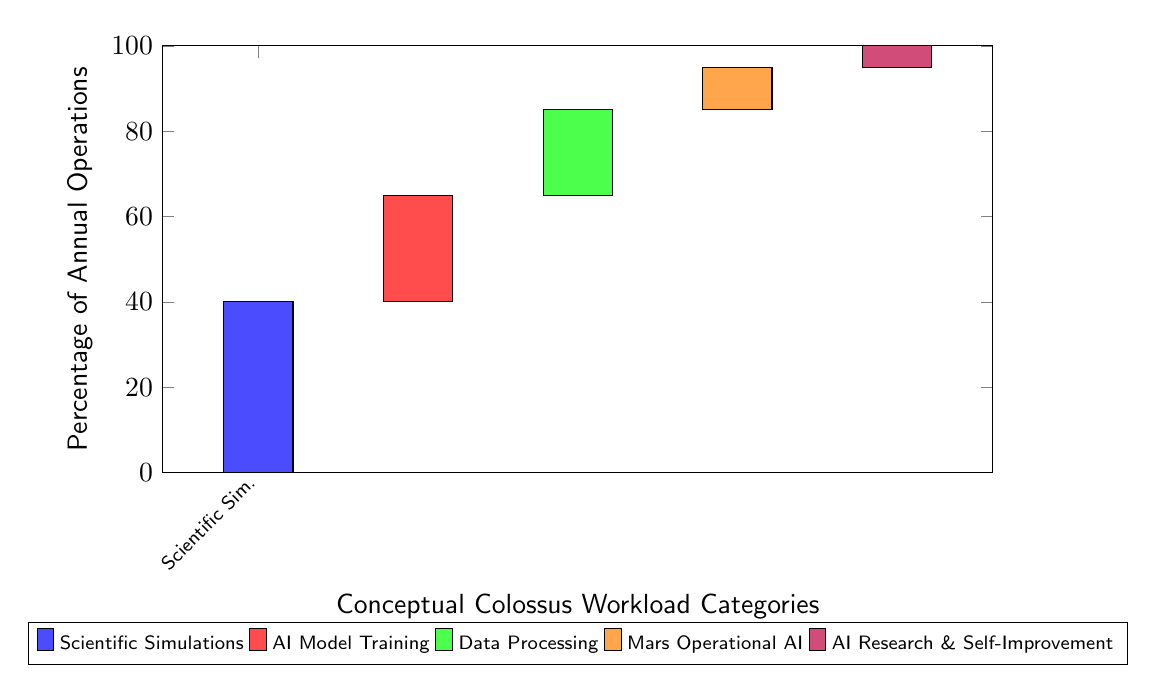
\begin{tikzpicture}
  \begin{axis}[
      ybar stacked,
      xlabel={Conceptual Colossus Workload Categories},
      ylabel={Percentage of Annual Operations},
      symbolic x coords={Scientific Sim., AI Model Training, Data Processing, Mars Ops AI, AI R\&D},
      xtick=data,
      xticklabel style={rotate=45, anchor=east, font=\scriptsize},
      ymin=0, ymax=100,
      bar width=25pt,
      enlarge x limits=0.15,
      legend style={at={(0.5,-0.35)}, anchor=north, legend columns=-1, font=\scriptsize},
      title style={font=\small},
      width=\textwidth,
      height=7cm
    ]
    \addplot[fill=blue!70] coordinates {(Scientific Sim., 40)};
    \addlegendentry{Scientific Simulations}
    \addplot[fill=red!70] coordinates {(AI Model Training, 25)};
    \addlegendentry{AI Model Training}
    \addplot[fill=green!70] coordinates {(Data Processing, 20)};
    \addlegendentry{Data Processing}
    \addplot[fill=orange!70] coordinates {(Mars Ops AI, 10)};
    \addlegendentry{Mars Operational AI}
    \addplot[fill=purple!70] coordinates {(AI R\&D, 5)};
    \addlegendentry{AI Research \& Self-Improvement}
  \end{axis}
\end{tikzpicture}
\noindent\footnotesize
\textbf{Source Note:}\\[0.5em]
This chart provides a conceptual breakdown of how the 2.5 quadrillion annual operations from the Colossus AI data center might be allocated across different workload categories. The percentages are illustrative and subject to change based on strategic priorities and demand. Data for specific AI workload energy consumption trends for training versus inference can be found in Desislavov, R., et al. (2023).\footnote{Desislavov, Radosvet, Fernando Mart´ınez-Plumed, and Jos´e Hern´andez-Orallo. ``Compute and Energy Consumption Trends in Deep Learning Inference.'' \textit{arXiv preprint arXiv:2109.05472}, 2023. 







\href{https://arxiv.org/pdf/2109.05472}\url{https://arxiv.org/pdf/2109.05472}} The AI Work Quantization Model offers a framework for more granular quantification of diverse AI tasks.\footnote{Aasish Kumar Sharma, Michael Bidollahkhani, and Julian Martin Kunkel. ``AI Work Quantization Model: Closed-System AI Computational Effort Metric.'' arXiv preprint arXiv:2503.14515 (2025). 







\href{https://arxiv.org/pdf/2503.14515}\url{https://arxiv.org/pdf/2503.14515}}

\medskip

\noindent
This initial monetization through Earth contracts, driven by Colossus's quantifiable output, marks the first step towards building a robust, self-sustaining Martian economy, transitioning to supporting local needs and further interplanetary expansion.



\subsection*{VI.5. Transition to a Local Martian Economy}

\addcontentsline{toc}{subsection}{VI.5. Transition to a Local Martian Economy} 


The strategic imperative for the Martian settlement extends beyond mere survival to achieving economic self-sufficiency. Initial mission phases rely on Earth-based investment and resources, primarily generated through contracts leveraging the unique computational capabilities of the Colossus AI data center.\footnote{J. S. McNatt, ``Photovoltaics and Power to Support NASA’s Moon to Mars Objectives,'' presented at the 28th Space Photovoltaic Research and Technology Conference, Cleveland, Ohio, Sep. 4, 2024, p. 3. Available: 







\href{https://ntrs.nasa.gov/api/citations/20240010682/downloads/PV\%20and\%20Power\%20to\%20Support\%20NASA\%20M2M.pdf}\url{https://ntrs.nasa.gov/api/citations/20240010682/downloads/PV\%20and\%20Power\%20to\%20Support\%20NASA\%20M2M.pdf}} A long-term, sustainable presence requires a fundamental transition to a self-sustaining local Martian economy.

\medskip

\noindent
This transition involves cultivating internal value chains and reducing dependence on Earth imports. The defined resource units---Computational Units (CUs), Discovery Units (DUs), Operational Units (OUs), and Data Access Units (DAUs)---serve as the foundational elements for internal value exchange and resource allocation within the growing colony. CUs represent processing power, DUs quantify the value of new knowledge and breakthroughs, OUs measure the contribution of labor (both human and robotic), and DAUs govern access to critical information stores. These units facilitate trade, compensation, and investment decisions within the Martian system, distinct from Earth-based currencies.

\medskip

\noindent
Economic diversification is paramount to achieving self-sufficiency. While computational services provide initial external revenue, the local economy must broaden its base by leveraging In-Situ Resource Utilization (ISRU) and local manufacturing capabilities.\footnote{National Aeronautics and Space Administration, ``Moon to Mars Objectives,'' September 2022, p. 9, 







\href{https://www.nasa.gov/wp-content/uploads/2022/09/m2m-objectives-exec-summary.pdf}\url{https://www.nasa.gov/wp-content/uploads/2022/09/m2m-objectives-exec-summary.pdf}} Resources such as regolith and water ice, extracted and processed using energy from the expanding Martian Energy Grid,\footnote{J. S. McNatt, ``Photovoltaics and Power to Support NASA’s Moon to Mars Objectives,'' presented at the 28th Space Photovoltaic Research and Technology Conference, Cleveland, Ohio, Sep. 4, 2024, p. 3. Available: 







\href{https://ntrs.nasa.gov/api/citations/20240010682/downloads/PV\%20and\%20Power\%20to\%20Support\%20NASA\%20M2M.pdf}\url{https://ntrs.nasa.gov/api/citations/20240010682/downloads/PV\%20and\%20Power\%20to\%20Support\%20NASA\%20M2M.pdf}} form the basis for local industries producing construction materials, consumables, and manufacturing feedstocks. Local production, enabled by advancements in Martian Fabrication,\footnote{Lucas-Stannard, P., \& Lasslop, A. (Eds.). (2006). \textit{Mars Settlement and Society Working Group Report}. Next Generation Exploration Conference 2006, 







\href{https://ntrs.nasa.gov/api/citations/20070008279/downloads/20070008279.pdf}\url{https://ntrs.nasa.gov/api/citations/20070008279/downloads/20070008279.pdf}} supports local infrastructure development and reduces the mass and cost burden of Earth resupply.

\medskip

\noindent
The robotic workforce, directed by AI and human oversight, provides the labor (OUs) for these nascent industries, while human ingenuity drives scientific research (generating DUs) and operational improvements (reducing OU requirements). This interaction between Colossus-generated CUs, ISRU-derived materials, robot-provided OUs, and human/AI-driven DUs and DAUs creates internal economic cycles. Resource Valorization, the process of assigning value to locally sourced and processed materials and services, further strengthens the local economy. The positive feedback system of expanding infrastructure (powered by the Grid), increasing AI capability (Colossus Deployment), growing workforce (human and robotic), and diversified local production constitutes the Systemic Expansion Engine, propelling the colony towards Exponential Scaling of its capabilities and independence.

\medskip

\noindent


\begin{figure}[H]
  \centering
  \noindent
  \begin{minipage}{\textwidth}
    \centering
    \adjincludegraphics[
      max size={\textwidth}{0.9\textheight},
      keepaspectratio
    ]{images/inline-diagram-2426709979}
    \caption{This diagram illustrates the flow of resource units (Computational, Research, Operational, Data Access) within the developing Martian economy.}
  \end{minipage}
\end{figure}

\begin{comment}
@startuml
!theme materia-outline
scale 1.6

skinparam defaultFontColor black
skinparam backgroundColor white


scale 1.6

skinparam defaultFontColor black
skinparam backgroundColor white



title ``Martian Economy:\nResource Unit Flow''

skinparam rectangle {
  BorderColor black
  FontColor black
  shadowing 0
  FontSize 10
}
skinparam component {
  BorderColor black
  FontColor black
  shadowing 0
  FontSize 12
}
skinparam arrow {
  Color black
}

component ``Colossus AI\n(CU Source)'' as Colossus
component ``Sci/Research\n(DU Source)'' as Science
component ``Workforce\n(OU Source)'' as Workforce
component ``Data Sources\n(DAU Source)'' as DataSources

rectangle ``Comp. Units\n(CU)'' as CU
rectangle ``Disc. Units\n(DU)'' as DU
rectangle ``Oper. Units\n(OU)'' as OU
rectangle ``Data Access\nUnits (DAU)'' as DAU

component ``Martian\nEconomy'' as Economy

component ``Earth\nClients'' as EarthClients
component ``ISRU/\nMfg'' as ISRUMfg
component ``Interplanetary\nExpansion'' as Expansion


Colossus --> CU : ``Generates''
Science --> DU : ``Generates''
Workforce --> OU : ``Generates''
DataSources --> DAU : ``Generates''

CU --> Economy : ``Flows to''
DU --> Economy : ``Flows to''
OU --> Economy : ``Flows to''
DAU --> Economy : ``Flows to''

Economy --> EarthClients : ``CUs\n(External Value)''
Economy --> ISRUMfg : ``OUs\n(Internal Use)''
Economy --> Expansion : ``Fuels''

ISRUMfg --> Economy : ``Materials/\nFeedstock''

note right of Economy
  Internal Exchange
  Trade
  Allocation
end note

@enduml
\end{comment}



\medskip

\noindent
The success of this transition to a self-sufficient Martian economy, both in terms of internal prosperity and continued external competitiveness, depends on achieving ambitious efficiency gains across all operations.



\subsection*{VI.6. Analysis of Efficiency Gains}

\addcontentsline{toc}{subsection}{VI.6. Analysis of Efficiency Gains} 


\medskip

\noindent
The economic viability of the Martian enterprise, and its capacity to fuel the Systemic Expansion Engine, is inextricably linked to achieving significant efficiency gains in its core computational infrastructure. A targeted 80\% annual efficiency gain in computational output per unit cost is a foundational assumption of this plan. This translates to the cost of producing a standardized unit of computational output decreasing to 20\% of its value from the preceding year, or, equivalently, a fivefold increase in computational output for the same unit cost, year over year. This rate of improvement is essential for maintaining competitiveness against Earth-based AI services, funding colony growth, and achieving the Exponential Scaling necessary for interplanetary operations.

\medskip

\noindent
This target is driven by a confluence of factors:
\begin{itemize}
    \item \textbf{Improved AI Models:} Continuous advancements in AI algorithms, model architectures, and training methodologies yield increases in problem-solving capability per computational operation. This includes breakthroughs in algorithmic efficiency, such as sparse attention mechanisms that offer speedups for transformer models\footnote{Jingyang Yuan, et al. ``Native Sparse Attention: A Key to Scalable and Efficient Generative Transformers.'' arXiv:2502.11089, 2025. 















\href{https://arxiv.org/pdf/2502.11089}\url{https://arxiv.org/pdf/2502.11089}}, and the increased productivity observed in human-AI collaborative tasks\footnote{Dell’Acqua, Fabrizio, et al. ``Navigating the Jagged Technological Frontier: Field Experimental Evidence of the Effects of AI on Knowledge Worker Productivity and Quality.'' Working Paper 24-013, Harvard Business School, September 22, 2023. 















\href{https://www.hbs.edu/ris/Publication\%2520Files/24-013\_d9b45b68-9e74-42d6-a1c6-c72fb70c7282.pdf}\url{https://www.hbs.edu/ris/Publication\%2520Files/24-013\_d9b45b68-9e74-42d6-a1c6-c72fb70c7282.pdf}}.
    \item \textbf{Better Hardware:} While initially reliant on Earth-produced, Mars-hardened chips (Dojo, GPUs), ongoing advancements in semiconductor design, architecture optimization (e.g., Processing-in-Memory (PIM) architectures showing promise for LLM inference efficiency\footnote{Cristobal Ortega, Yann Falevoz, Renaud Ayrignac. ``PIM-AI: A Novel Architecture for High-Efficiency LLM Inference.'' arXiv:2411.17309 [cs.AR], November 2024. 















\href{https://arxiv.org/pdf/2411.17309}\url{https://arxiv.org/pdf/2411.17309}}), and system-level integration contribute to increased raw processing power per watt and per dollar.
    \item \textbf{Enhanced Software:} Optimizations in compilers, runtime environments, distributed computing frameworks, and operating systems specifically tailored for the Colossus architecture and Martian operational constraints unlock further performance gains from the hardware.
    \item \textbf{Competitive Pressure:} The dynamic landscape of Earth-based AI services provides a strong impetus for Mars to achieve and maintain a competitive edge, driving relentless innovation in efficiency.
\end{itemize}

\medskip

\noindent
Measuring and validating this efficiency gain requires a rigorous approach beyond raw FLOPS. The AI Workload Quantization Metric (AWQM) offers a framework to quantify computational effort across diverse hardware and tasks, correlating AI workload units to human labor equivalence (e.g., 5 AWQM units $\approx$ 60--72 human-hours)\footnote{Aasish Kumar Sharma, Michael Bidollahkhani, and Julian Martin Kunkel. ``AI Work Quantization Model: Closed-System AI Computational Effort Metric.'' arXiv preprint arXiv:2503.14515 (2025). 















\href{https://arxiv.org/pdf/2503.14515}\url{https://arxiv.org/pdf/2503.14515}}. This allows for tracking the increasing \textit{value} of computational output. Additionally, metrics like Compute Carbon Intensity (CCI), measuring grams of CO2-equivalent per ExaFLOP\footnote{Ibid.}, link computational efficiency to energy consumption and sustainability, crucial for the solar-powered Martian Energy Grid. Hardware benchmarks (e.g., MLPerf, specific PIM-AI performance data), algorithmic speedup metrics, and human-AI productivity metrics are continuously monitored via real-time operational dashboards.

\medskip

\noindent
The relationship between an annual efficiency gain ($E_{\text{gain}}$) and the reduction in cost ($C_t$) for a constant unit of computational output over time ($t$ in years) can be modeled as:
\begin{equation}
C_t = C_0 \times (1 - E_{\text{gain}})^t
\end{equation}
For the targeted 80\% efficiency gain ($E_{\text{gain}} = 0.8$), this means $C_t = C_0 \times (0.2)^t$. The projected impact of this on the normalized cost per Computational Unit is illustrated below, showing a dramatically steeper cost reduction compared to more conservative gain scenarios.

\begin{figure}[H]
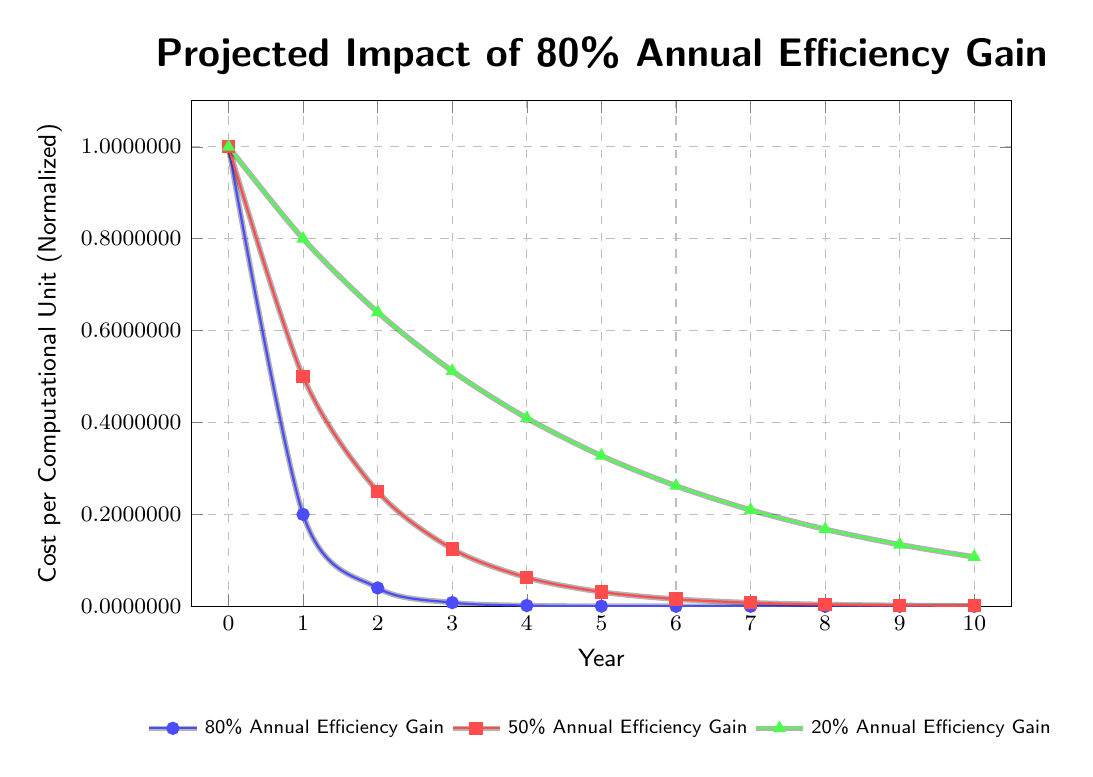
\begin{tikzpicture}
  \begin{axis}[
    width=12cm,
    height=8cm,
    xlabel={Year},
    ylabel={Cost per Computational Unit (Normalized)},
    title={Projected Impact of 80\% Annual Efficiency Gain},
    title style={font=\bfseries\Large},
    grid=major,
    grid style={dashed, gray!50},
    axis background/.style={fill=white},
    legend style={
      at={(0.5,-0.2)}, 
      anchor=north,
      legend columns=-1,
      draw=none,
      font=\scriptsize 
    },
    tick label style={font=\footnotesize},
    label style={font=\small},
    enlarge x limits=0.05,
    ymin=0,
    xtick={0,1,2,3,4,5,6,7,8,9,10},
    yticklabel style={/pgf/number format/.cd,fixed,fixed zerofill,precision=7,/tikz/.cd}
  ]
  
  \addplot[
    smooth,
    thick,
    color=blue!70,
    mark=*, mark options={fill=blue!70},
    preaction={draw=black, line width=2pt, opacity=0.3}
  ] coordinates {
    (0, 1.0) (1, 0.2) (2, 0.04) (3, 0.008) (4, 0.0016) (5, 0.00032) (6, 0.000064) (7, 0.0000128) (8, 0.00000256) (9, 0.000000512) (10, 0.0000001024)
  };
  \addlegendentry{80\% Annual Efficiency Gain}
  
  \addplot[
    smooth,
    thick,
    color=red!70,
    mark=square*, mark options={fill=red!70},
    preaction={draw=black, line width=2pt, opacity=0.3}
  ] coordinates {
    (0, 1.0) (1, 0.5) (2, 0.25) (3, 0.125) (4, 0.0625) (5, 0.03125) (6, 0.015625) (7, 0.0078125) (8, 0.00390625) (9, 0.001953125) (10, 0.0009765625)
  };
  \addlegendentry{50\% Annual Efficiency Gain}

  \addplot[
    smooth,
    thick,
    color=green!70,
    mark=triangle*, mark options={fill=green!70},
    preaction={draw=black, line width=2pt, opacity=0.3}
  ] coordinates {
    (0, 1.0) (1, 0.8) (2, 0.64) (3, 0.512) (4, 0.4096) (5, 0.32768) (6, 0.262144) (7, 0.2097152) (8, 0.16777216) (9, 0.134217728) (10, 0.1073741824)
  };
  \addlegendentry{20\% Annual Efficiency Gain}
  
  \end{axis}
\end{tikzpicture}
\noindent\footnotesize
This line chart illustrates the projected cost per computational unit over 10 years under different annual efficiency gain scenarios, normalized to Year 0 cost. The 80\% target demonstrates a significantly steeper cost reduction curve.
\end{figure}

\medskip

\noindent
Achieving such gains necessitates continuous innovation. AI-driven predictive efficiency modeling forecasts trends, while cross-factor efficiency optimization identifies synergistic improvements across AI models, hardware, and software. Further refining resource units to be energy-cost-aware (integrating CCI with CUs/PHEs) and quantifying discovery efficiency (e.g., DUs generated per CU consumed) provide granular insights. Modeling the impact of the Martian environment (radiation, dust, thermal cycles) on hardware and software efficiency is crucial for realistic projections and adaptive management. This pursuit of efficiency is paramount for the economic viability and growth of the Martian enterprise.



\subsection*{VI.7. Pricing and Allocation Mechanisms}

\addcontentsline{toc}{subsection}{VI.7. Pricing and Allocation Mechanisms} 


\medskip

\noindent
The Martian economic framework requires robust mechanisms for pricing and allocating its diverse resource units: Computational Units (CUs), Discovery Units (DUs), Operational Units (OUs), and Data Access Units (DAUs). These systems are essential for Resource Valorization, supporting the transition to a local Martian economy and powering the Systemic Expansion Engine.

\medskip

\noindent
Dynamic pricing models determine the value of these resource units based on several factors:
\begin{itemize}
    \item \textbf{Demand:} Requests from internal stakeholders (humans, AI systems, research projects) and external clients (Earth contracts) directly influence prices. High demand for specific computational tasks or critical discoveries increases value.
    \item \textbf{Availability:} The operational status of the Martian Energy Grid, Colossus, the robotic workforce, and specific datasets impacts supply and thus price. Scarcity, whether temporary or systemic, raises unit prices.
    \item \textbf{Strategic Priorities:} The colony's goals, such as accelerating research or prioritizing infrastructure, can influence pricing and allocation tiers.
\end{itemize}
AI systems are integral to dynamic pricing, analyzing real-time data to adjust prices algorithmically, optimizing resource use across the economy.\footnote{A. A. Baktayan and I. A. Al-Baltah, ``A Survey on Intelligent Computation Offloading and Pricing Strategy in UAV-Enabled MEC Network: Challenges and Research Directions,'' \textit{arXiv preprint arXiv:2208.10072}, 2022. 







\href{https://arxiv.org/pdf/2208.10072}\url{https://arxiv.org/pdf/2208.10072}}

\medskip

\noindent
Resource allocation to diverse stakeholders is managed through a transparent framework. Stakeholders submit requests detailing their needs. High-level allocation decisions, especially for large resource blocks or strategic priorities, are overseen by Expertise-Weighted Councils.\footnote{Lucas-Stannard, P., \& Lasslop, A. (Eds.). (2006). \textit{Mars Settlement and Society Working Group Report}. Next Generation Exploration Conference 2006, p. 5. 







\href{https://ntrs.nasa.gov/api/citations/20070008279/downloads/20070008279.pdf}\url{https://ntrs.nasa.gov/api/citations/20070008279/downloads/20070008279.pdf}} These councils, including human and potentially AI representatives, ensure alignment with colony objectives. Allocation may be weighted by contribution, linking resource access to value creation in the Resource-Based Value System.

\medskip

\noindent
Transparency and fairness are essential. Transparent accounting systems track resource generation, pricing, requests, and allocations. A decentralized ledger, potentially using blockchain or DAG technology, provides an immutable, auditable record. This system supports the accountability of allocation decisions. AI models monitor allocation patterns for biases, promoting distribution. Automated smart contracts on the ledger can execute predefined allocation rules based on milestones or trigger conditions, enhancing efficiency. These mechanisms ensure that the economy operates efficiently, supporting the diverse needs of human, AI, and robotic inhabitants and driving mission success.

\medskip



\begin{figure}[H]
  \centering
  \noindent
  \begin{minipage}{\textwidth}
    \centering
    \adjincludegraphics[
      max size={\textwidth}{0.9\textheight},
      keepaspectratio
    ]{images/inline-diagram-1179343416}
    \caption{This diagram illustrates the process for pricing and allocating computational, research, operational, and data resources within the Martian economy, exhibiting inputs such as resource units, demand signals, availability, and strategic priorities, and outputs including allocations to various stakeholders (humans, AI systems, research projects, commercial entities). The roles of AI-driven dynamic pricing, Expertise-Weighted Councils, and transparent accounting systems (potentially via a decentralized ledger) are central to this process.}
  \end{minipage}
\end{figure}

\begin{comment}
@startuml
!theme cloudscape-design
scale 1.6

skinparam defaultFontColor black
skinparam backgroundColor white



title ``Martian Resource\nPricing & Allocation''

skinparam rectangle {
  BorderColor black
  FontColor black
  shadowing 0
  FontSize 12
}
skinparam component {
  BorderColor black
  FontColor black
  shadowing 0
  FontSize 12
}
skinparam package {
  BorderColor black
  BackgroundColor #ADD8E6
  FontColor black
  shadowing 0
  StereotypeFontSize 0
}
skinparam arrow {
  Color black
}


rectangle ``Resource Units\n(CU, DU, OU, DAU)'' as Units
rectangle ``Demand Signals'' as Demand
rectangle ``Availability'' as Avail
rectangle ``Strategic\nPriorities'' as Priority

component ``Resource\nRequests'' as Requests
component ``AI Dynamic\nPricing'' as AIDP
component ``Allocation\nProposal'' as Proposal
component ``Expertise-Weighted\nCouncils'' as Councils
rectangle ``Final\nAllocations'' as FinalAlloc
component ``Transparent\nLedger'' as Ledger

package ``Stakeholders'' as StakeholdersPkg {
    rectangle ``Humans'' as Human
    rectangle ``AI Systems'' as AI
    rectangle ``Research\nProjects'' as Research
    rectangle ``Commercial\nEntities'' as Commercial
}

' Inputs to Requests
Units --> Requests : ``Form''
Demand --> Requests : ``Form''
Avail --> Requests : ``Form''
Priority --> AIDP : ``Influence''

' Requests and Inputs to AI Pricing
Requests --> AIDP : ``Input to''

' AI Pricing to Proposal
AIDP --> Proposal : ``Generates''

' Proposal to Review or Finalization
Proposal --> Councils : ``Strategic\nReview''
Proposal --> FinalAlloc : ``Direct Path\n(No Review)''

' Councils to Final Allocation
Councils --> FinalAlloc : ``Approved\nProposal''

' Final Allocation to Ledger
FinalAlloc --> Ledger : ``Recorded in''

' Ledger to Stakeholders (Output)
Ledger --> StakeholdersPkg : ``Distributed to''

' Stakeholders breakdown
StakeholdersPkg --> Human
StakeholdersPkg --> AI
StakeholdersPkg --> Research
StakeholdersPkg --> Commercial

note bottom of AIDP
  Analyzes
  Real-time Data
end note

note bottom of Councils
  High-level
  Decisions
end note

note bottom of Ledger
  Immutable
  Auditable
end note

@enduml
\end{comment}




            
\section*{References}

\addcontentsline{toc}{section}{References} 


\subsection*{References and More Information:}

\addcontentsline{toc}{subsection}{References and More Information:} 


\noindent \textbf{Abel, P. B., Anderson, M. D., Blom, E. T., Calle, C., Dunlap, P. H., Greenberg, P. S., Fischer, D. G., Howard, S. A., Hurlbert, K. M., Jordan, J. L., Ludwiczak, D. R., Orndoff, E., Thomas, F., \& Wohl, C. J.} (2023). \textit{Lunar Dust Mitigation: A Guide and Reference First Edition (2021)}. National Aeronautics and Space Administration. NASA/TP-20220018746. Available from NASA Technical Reports Server. This document contributed information regarding the challenges of lunar dust mitigation and potential strategies, informing the discussion of dust mitigation for solar arrays on Mars. 



\href{https://ntrs.nasa.gov/api/citations/20220018746/downloads/TP-20220018746.pdf}{\url{https://ntrs.nasa.gov/api/citations/20220018746/downloads/TP-20220018746.pdf}}

\vspace{1em}
\noindent \textbf{Appelbaum, Joseph, and Dennis J. Flood.} (1989). \textit{Solar Radiation on Mars} (NASA Technical Memorandum 102299, E-4865). Lewis Research Center, Cleveland, Ohio. Retrieved from NASA Technical Reports Server. This foundational work provided critical data and methodology for calculating solar irradiance on Mars, including the impact of atmospheric dust and dust storms, essential for estimating solar energy generation potential for the Martian Energy Grid. 



\href{https://ntrs.nasa.gov/api/citations/19890018252/downloads/19890018252.pdf}{\url{https://ntrs.nasa.gov/api/citations/19890018252/downloads/19890018252.pdf}}

\vspace{1em}
\noindent \textbf{Baktayan, A. A., and I. A. Al-Baltah.} (2022). ``A Survey on Intelligent Computation Offloading and Pricing Strategy in UAV-Enabled MEC Network: Challenges and Research Directions.'' \textit{arXiv preprint arXiv:2208.10072}. This survey contributed insights into dynamic pricing and resource allocation strategies using AI methods, which informed the discussion on economic models and resource management for the Martian computational economy. 



\href{https://arxiv.org/pdf/2208.10072}{\url{https://arxiv.org/pdf/2208.10072}}

\vspace{1em}
\noindent \textbf{Barker, Jamen W.} (2025). ``The Psychological Effects of ICE Conditions in Long-Term Space Travel.'' Brigham Young University. Available from BYU ScholarsArchive. This student paper provided information on the psychological challenges of long-duration space missions, including communication latency, which informed the discussion on Martian Governance Autonomy and the need for local authority. 



\href{https://scholarsarchive.byu.edu/studentpub/402}{\url{https://scholarsarchive.byu.edu/studentpub/402}}

\vspace{1em}
\noindent \textbf{Bazilian, Morgan, Ian Christensen, Ian Lange, George Sowers, and Angel Abbud-Madrid.} (2019). ``New Policies Needed to Advance Space Mining.'' \textit{Issues in Science and Technology} 35, no. 2: 26--30. This article provided context on the nascent economics of space mining and the development of legal frameworks for space resource utilization, informing the discussion on interplanetary expansion and the economic viability of leveraging asteroid resources. 



\href{https://issues.org/new-policies-needed-to-advance-space-mining/}{\url{https://issues.org/new-policies-needed-to-advance-space-mining/}}

\vspace{1em}
\noindent \textbf{Cascade Team.} (2023, January 27, Updated June 7). ``4-Step Strategy Reporting Process (With Template).'' \textit{Cascade}. This resource provided insights into strategy reporting and dashboard visualization, informing the discussion on Phase Gates and Milestone Validation and the use of operational data analysis. 



\href{https://www.cascade.app/blog/strategy-reporting}{\url{https://www.cascade.app/blog/strategy-reporting}}

\vspace{1em}
\noindent \textbf{Carniti, P., Gotti, C., \& Pessina, G.} (2024). ``A Multi-Function Radiation-Hardened HV and LV Linear Regulator for SiPM-based HEP Detectors.'' \textit{arXiv preprint arXiv:2402.08297}. This paper contributed technical details on radiation hardening by design techniques for semiconductor devices, informing the discussion on radiation hardening for critical components in the Martian environment. 



\href{https://arxiv.org/pdf/2402.08297}{\url{https://arxiv.org/pdf/2402.08297}}

\vspace{1em}
\noindent \textbf{Chappell, Michael B., Stephen Hoffman, and Omar Bekdash.} (2021). ``Human Mars Mission Surface Power Impacts on Timeline and Traverse Capabilities.'' \textit{2021 IEEE Aerospace Conference (50100)}. IEEE. Available from NASA Technical Reports Server. This conference paper provided data on initial power requirements for minimal human Mars missions and the impact of power on surface operations timelines, informing the discussion on Phase 1 foundational infrastructure deployment. 



\href{https://ntrs.nasa.gov/api/citations/20210022250/downloads/MarsSurfacePowerOps\_IEEE\_final.pdf}{\url{https://ntrs.nasa.gov/api/citations/20210022250/downloads/MarsSurfacePowerOps\_IEEE\_final.pdf}}

\vspace{1em}
\noindent \textbf{Colgan, N., Nellis, G., \& Anderson, M.} (2021). ``Forced Convection Heat Rejection System for Mars Surface Applications.'' \textit{Workshop on Spacecraft Charging}. Presented at Wisconsin Space Conference 2021. Available from Carthage College OJS. This paper provided data and analysis on the performance of forced convection heat exchangers for waste heat rejection in the thin Martian atmosphere, informing the discussion on waste heat rejection systems for Colossus. 



\href{https://dione.carthage.edu/ojs/index.php/wsc/article/download/344/340}{\url{https://dione.carthage.edu/ojs/index.php/wsc/article/download/344/340}}

\vspace{1em}
\noindent \textbf{Colgan, N., Nellis, G., \& Anderson, M.} (2022). ``Forced Convection Heat Rejection System for Mars Surface Applications.'' \textit{Proceedings of the Wisconsin Space Conference}, 1(1). This article provided updated data and analysis on the optimal design and performance of forced convection heat exchangers for Mars, reinforcing the findings from the 2021 conference presentation and informing the discussion on waste heat rejection systems. 



\href{https://doi.org/10.17307/wsc.v1i1.344}{\url{https://doi.org/10.17307/wsc.v1i1.344}}

\vspace{1em}
\noindent \textbf{Dell’Acqua, Fabrizio, et al.} (2023, September 22). ``Navigating the Jagged Technological Frontier: Field Experimental Evidence of the Effects of AI on Knowledge Worker Productivity and Quality.'' \textit{Working Paper 24-013}. Harvard Business School. This working paper provided insights into the impact of AI on knowledge worker productivity and the concept of the ``jagged technological frontier,'' informing the discussion on Scientific Acceleration and Human-AI-Robot Synergy. 



\href{https://www.hbs.edu/ris/Publication\%2520Files/24-013\_d9b45b68-9e74-42d6-a1c6-c72fb70c7282.pdf}{\url{https://www.hbs.edu/ris/Publication\%2520Files/24-013\_d9b45b68-9e74-42d6-a1c6-c72fb70c7282.pdf}}

\vspace{1em}
\noindent \textbf{Desislavov, Radosvet, Fernando Mart´ınez-Plumed, and Jos´e Hern´andez-Orallo.} (2023). ``Compute and Energy Consumption Trends in Deep Learning Inference.'' \textit{arXiv preprint arXiv:2109.05472}. This preprint provided data and analysis on energy consumption trends in deep learning inference and the impact of hardware efficiency, informing the discussion on Economic Viability and efficiency gains for Colossus. 



\href{https://arxiv.org/pdf/2109.05472}{\url{https://arxiv.org/pdf/2109.05472}}

\vspace{1em}
\noindent \textbf{Djorgovski, S. G., A. A. Mahabal, M. J. Graham, K. Polsterer, A. Krone-Martins.} (2022). ``Applications of AI in Astronomy.'' \textit{arXiv preprint arXiv:2212.01493}. To appear in: Artificial Intelligence for Science, eds. A. Choudhary, G. Fox and T. Hey. Singapore: World Scientific, in press (2023). This preprint provided a comprehensive overview of AI applications in astronomical data analysis, including the growth of relevant literature and the use of AI for tasks like classification and anomaly detection, informing the discussion on Scientific Acceleration and Adaptive Risk Management. 



\href{https://arxiv.org/pdf/2212.01493}{\url{https://arxiv.org/pdf/2212.01493}}

\vspace{1em}
\noindent \textbf{Dodig-Crnkovic, Gordana.} (2023). \textit{Computational Natural Philosophy: A Thread from Presocratics through Turing to ChatGPT}. arXiv. This preprint provided a philosophical and historical context for an informational and computational view of the universe, informing the discussion on Scientific Acceleration. 



\href{https://arxiv.org/pdf/2309.13094}{\url{https://arxiv.org/pdf/2309.13094}}

\vspace{1em}
\noindent \textbf{Edwards, B. L.} (2024, November). ``Unlocking New Capabilities in Space Communications for NASA.'' NASA Space Technology Mission Directorate. Retrieved from NASA Technical Reports Server. This presentation provided data on communication challenges with Mars and NASA's goals for future data rates, informing the discussion on Introduction, Phased Implementation, and Phase Gates. 



\href{https://ntrs.nasa.gov/api/citations/20240013248/downloads/Edwards\%20Presentation\_Ver\%202.pdf}{\url{https://ntrs.nasa.gov/api/citations/20240013248/downloads/Edwards\%20Presentation\%20Ver\%202.pdf}}

\vspace{1em}
\noindent \textbf{Elon Musk.} (2025, March 14). ``Starship departs for Mars at the end of next year ...'' X. This social media post provided Elon Musk's projected timeline for Starship missions and potential human landings on Mars, informing the discussion on Phase 1 implementation timeline. 



\href{https://x.com/elonmusk/status/1900774290682683612}{\url{https://x.com/elonmusk/status/1900774290682683612}}

\vspace{1em}
\noindent \textbf{Goodrich, Michael A., and Alan C. Schultz.} (2007). ``Human–Robot Interaction: A Survey.'' Faculty Publications. 940. Available from BYU ScholarsArchive. This survey paper provided foundational insights into human-robot interaction, informing the discussion on Synergy, Optimization, and Learning and Human-AI-Robot Synergy. 



\href{https://scholarsarchive.byu.edu/facpub/940}{\url{https://scholarsarchive.byu.edu/facpub/940}}

\vspace{1em}
\noindent \textbf{Grand View Research.} (n.d.). ``AI Datasets \& Licensing For Academic Research And Publishing Market Report 2030.'' This market report provided information on the market for AI datasets and licensing in academic research, informing the discussion on Economic Viability and the monetization of AI-assisted scientific discoveries. 



\href{https://www.grandviewresearch.com/industry-analysis/ai-datasets-licensing-academic-research-publishing-market-report}{\url{https://www.grandviewresearch.com/industry-analysis/ai-datasets-licensing-academic-research-publishing-market-report}}

\vspace{1em}
\noindent \textbf{Händler, Thorsten.} (2023). ``Balancing Autonomy and Alignment: A Multi-Dimensional Taxonomy For Autonomous LLM-Powered Multi-Agent Architectures.'' \textit{arXiv preprint arXiv:2310.03659}. This preprint provided a taxonomy and analysis of AI alignment in multi-agent systems, informing the discussions on Martian Governance Autonomy, Synergy, Optimization, and Learning, and Phase Gates and Milestone Validation regarding AI safety metrics. 



\href{http://arxiv.org/pdf/2310.03659}{\url{http://arxiv.org/pdf/2310.03659}}

\vspace{1em}
\noindent \textbf{Jenkins, P., et al.} (2002). ``A Dust Characterization Experiment for Solar Cells Operating on Mars.'' NASA Glenn Research Center. Available from NASA Technical Reports Server. This paper provided specific data on dust deposition rates on Mars solar arrays observed during the Pathfinder mission, informing the discussion on Dust Impact and Mitigation. 



\href{https://ntrs.nasa.gov/api/citations/20020031145/downloads/20020031145.pdf}{\url{https://ntrs.nasa.gov/api/citations/20020031145/downloads/20020031145.pdf}}

\vspace{1em}
\noindent \textbf{Jones, H. W.} (2016). ``Humans to Mars Will Cost About ``Half a Trillion Dollars'' and Life Support Roughly Two Billion Dollars.'' \textit{46th International Conference on Environmental Systems}, Vienna, Austria. ICES-2016-111. Retrieved from NASA Technical Reports Server. This paper provided estimates for the initial mission mass requirements for human Mars exploration in Low Earth Orbit, informing the Introduction section's scale assessment. 



\href{https://ntrs.nasa.gov/api/citations/20200000973/downloads/20200000973.pdf}{\url{https://ntrs.nasa.gov/api/citations/20200000973/downloads/20200000973.pdf}}

\vspace{1em}
\noindent \textbf{Landis, G. A., Kerslake, T. W., Jenkins, P. P., \& Scheiman, D. A.} (2004). \textit{Mars Solar Power} (NASA/TM—2004-213367, AIAA–2004–5555). Glenn Research Center, Cleveland, Ohio. Available from NASA Technical Reports Server. This technical memorandum provided crucial data and analysis on the challenges of solar power on Mars, including dust impacts, temperature effects, and radiation shielding, informing the discussions on Technical Feasibility, Adaptive Risk Management, and Dust Impact and Mitigation. 



\href{https://ntrs.nasa.gov/api/citations/20040191326/downloads/20040191326.pdf}{\url{https://ntrs.nasa.gov/api/citations/20040191326/downloads/20040191326.pdf}}

\vspace{1em}
\noindent \textbf{Lucas-Stannard, Paige, and Alex Lasslop, Lead Editors.} (2006). \textit{Mars Settlement and Society Working Group Report}. Next Generation Exploration Conference 2006. Available from NASA Technical Reports Server. This report provided foundational ideas and requirements for Mars settlement infrastructure and governance, including considerations for integrating AI and robots, informing the Abstract, Introduction, Phased Implementation, Martian Governance Autonomy, and Phase Gates sections. 



\href{https://ntrs.nasa.gov/api/citations/20070008279/downloads/20070008279.pdf}{\url{https://ntrs.nasa.gov/api/citations/20070008279/downloads/20070008279.pdf}}

\vspace{1em}
\noindent \textbf{Luxembourg – Input to the Working Group on Legal Aspects of Space Resource Activities, Committee on the Peaceful Uses of Outer Space, Legal Subcommittee, Sixty-third session, Vienna, 15–26 April 2024, Item 9 of the provisional agenda, A/AC.105/C.2/2024/CRP.29.} (2024, April 17). Available at UNOOSA. This submission provided insights into the legal frameworks for space resource utilization and the potential for economic value creation from space resources, informing the Abstract, Phased Implementation, and Economic Models sections. 



\href{https://www.unoosa.org/res/oosadoc/data/documents/2024/aac\_105c\_22024crp/aac\_105c\_2024crp\_29\_0\_html/AC105\_C2\_2024\_CRP29E.pdf}{\url{https://www.unoosa.org/res/oosadoc/data/documents/2024/aac\_105c\_2024crp/aac\_105c\_2024crp\_29\_0\_html/AC105\_C2\_2024\_CRP29E.pdf}}

\vspace{1em}
\noindent \textbf{Mason, Lee S.} (2006). ``A Comparison of Fission Power System Options for Lunar and Mars Surface Applications.'' NASA/TM—2006-214120. Glenn Research Center, Cleveland, Ohio. Prepared for the Space Technology and Applications International Forum (STAIF–2006). Available from NASA Technical Reports Server. This technical memorandum provided data and analysis on waste heat rejection systems for fission power on Mars and mass scaling for different power system options, informing the discussions on Waste Heat Rejection Systems and Technical Feasibility. 



\href{https://ntrs.nasa.gov/api/citations/20060011236/downloads/20060011236.pdf}{\url{https://ntrs.nasa.gov/api/citations/20060011236/downloads/20060011236.pdf}}

\vspace{1em}
\noindent \textbf{McNatt, J. S.} (2024, September 4). ``Photovoltaics and Power to Support NASA’s Moon to Mars Objectives.'' Presented at the 28th Space Photovoltaic Research and Technology Conference, Cleveland, Ohio. Retrieved from NASA Technical Reports Server. This presentation provided data on solar power requirements for Mars, energy storage needs, and technology gaps for ISRU-derived power, informing the Abstract, Introduction, Economic Viability, Technical Feasibility, Phase 2, and Phase Gates sections. 



\href{https://ntrs.nasa.gov/api/citations/20240010682/downloads/PV\%20and\%20Power\%20to\%20Support\%20NASA\%20M2M.pdf}{\url{https://ntrs.nasa.gov/api/citations/20240010682/downloads/PV\%20and\%20Power\%20to\%20Support\%20NASA\%20M2M.pdf}}

\vspace{1em}
\noindent \textbf{Mueller, Robert P.} (2017, March 6). ``Construction with Regolith.'' NASA Kennedy Space Center – Swamp Works. Presented at CLASS / SSERVI / FSI The Technology and Future of In-Situ Resource Utilization (ISRU) A Capstone Graduate Seminar. Orlando, FL. Available from NASA Technical Reports Server. This presentation provided data on Martian regolith composition, ISRU for construction materials, and the power requirements for ISRU processes, informing the discussions on Radiation Hardening and Martian Fabrication. 



\href{https://ntrs.nasa.gov/api/citations/20170002067/downloads/20170002067.pdf}{\url{https://ntrs.nasa.gov/api/citations/20170002067/downloads/20170002067.pdf}}

\vspace{1em}
\noindent \textbf{NASA.} (2024, December). ``Mars Surface Power Technology Decision.'' 2024 Moon to Mars Architecture Concept Review. Available from NASA. This document provided information on NASA's decision to select nuclear fission for primary Mars surface power and data on power requirements for different mission scales, informing the Introduction, Technical Feasibility, and Phase 1 sections. 



\href{https://www.nasa.gov/wp-content/uploads/2024/12/acr24-mars-surface-power-decision.pdf}{\url{https://www.nasa.gov/wp-content/uploads/2024/12/acr24-mars-surface-power-decision.pdf}}

\vspace{1em}
\noindent \textbf{NASA.} (2024, September). ``DATA SCIENCE LEARNING - Analyzing Proposed Mars Landing Sites.'' NASA Office of STEM Engagement Next Gen STEM. This educational document provided criteria for Mars landing sites, including the preference for latitudes with adequate sunlight for solar power, informing the discussion on Solar Energy Generation and Storage Scaling. 



\href{https://www.nasa.gov/wp-content/uploads/2024/09/dsl-analyzing-proposed-mars-landing-sites-final-8-23-24-508.pdf?emrc=9d7936}{\url{https://www.nasa.gov/wp-content/uploads/2024/09/dsl-analyzing-proposed-mars-landing-sites-final-8-23-24-508.pdf?emrc=9d7936}}

\vspace{1em}
\noindent \textbf{NASA.} (2022, September). ``Moon to Mars Objectives.'' This document outlined NASA's high-level objectives for Mars infrastructure, including power and communications, and introduced the concept of scalability as a recurring tenet, informing the Abstract, Introduction, Synergy, Optimization, and Learning, and Phase Gates sections. 



\href{https://www.nasa.gov/wp-content/uploads/2022/09/m2m-objectives-exec-summary.pdf}{\url{https://www.nasa.gov/wp-content/uploads/2022/09/m2m-objectives-exec-summary.pdf}}

\vspace{1em}
\noindent \textbf{NASA.} (2024, July). ``Civil Space Shortfall Descriptions July 2024.'' This report identified technological shortfalls in various areas of civil space, including advanced habitation systems and dust mitigation, informing the discussions on Technical Feasibility and Synergy, Optimization, and Learning. 



\href{https://www.nasa.gov/wp-content/uploads/2024/07/civil-space-shortfall-descriptions-july-2024.pdf?emrc=622753}{\url{https://www.nasa.gov/wp-content/uploads/2024/07/civil-space-shortfall-descriptions-july-2024.pdf?emrc=622753}}

\vspace{1em}
\noindent \textbf{NASA/CR—2018-219771.} (2018, March). \textit{Vision 2040: A Roadmap for Integrated, Multiscale Modeling and Simulation of Materials and Systems}. Available from NASA Technical Reports Server. This roadmap discussed the application of AI/ML in materials science research and data analysis, informing the discussions on Scientific Acceleration and Adaptive Risk Management regarding AI-driven analysis. 



\href{https://ntrs.nasa.gov/api/citations/20180002010/downloads/20180002010.pdf}{\url{https://ntrs.nasa.gov/api/citations/20180002010/downloads/20180002010.pdf}}

\vspace{1em}
\noindent \textbf{Oleson, Steven R., et al.} (2024). ``Kiloton Class ISRU Systems for LO2/LCH4 Propellant Production on the Mars Surface.'' In \textit{AIAA SciTech Forum}, Orlando, FL USA. Available from NASA Technical Reports Server. This paper provided detailed power requirements for large-scale Mars ISRU propellant production from water ice, informing the discussion on Martian Fabrication and Resource Utilization. 



\href{https://ntrs.nasa.gov/api/citations/20230017069/downloads/SciTech\%20Mars\%20kiloton\%20ISRU\%20Final.pdf}{\url{https://ntrs.nasa.gov/api/citations/20230017069/downloads/SciTech\%20Mars\%20kiloton\%20ISRU\%20Final.pdf}}

\vspace{1em}
\noindent \textbf{Ortega, Cristobal, Yann Falevoz, Renaud Ayrignac.} (2024, November). ``PIM-AI: A Novel Architecture for High-Efficiency LLM Inference.'' \textit{arXiv:2411.17309 [cs.AR]}. This preprint introduced a novel hardware architecture with potential for significant energy efficiency gains in AI inference, informing the discussion on Economic Viability and Analysis of Efficiency Gains. 



\href{https://arxiv.org/pdf/2411.17309}{\url{https://arxiv.org/pdf/2411.17309}}

\vspace{1em}
\noindent \textbf{Rucker, Michelle A.} (2016, December). ``Surface Power for Mars.'' Mars Study Capability Team, National Aeronautics and Space Administration. Presented at CLASS / SSERVI / FSI The Technology and Future of In-Situ Resource Utilization (ISRU) A Capstone Graduate Seminar. Orlando, FL. Available from NASA Technical Reports Server. This presentation provided conceptual analysis and data on Mars surface power requirements, including ISRU power needs, informing the discussion on Technical Feasibility. 



\href{https://ntrs.nasa.gov/api/citations/20160014032/downloads/20160014032.pdf}{\url{https://ntrs.nasa.gov/api/citations/20160014032/downloads/20160014032.pdf}}

\vspace{1em}
\noindent \textbf{Sanders, Gerald B.} (n.d.). ``Space Resources and Mining: Current Objectives, Plans, and Missions.'' NASA Johnson Space Center, Houston, TX, USA. Available from NASA Technical Reports Server. This document outlined NASA's objectives and plans for space resource utilization, highlighting the importance of ISRU for Earth independence, informing the Abstract and Synergy, Optimization, and Learning sections. 



\href{https://ntrs.nasa.gov/api/citations/20190001038/downloads/20190001038.pdf}{\url{https://ntrs.nasa.gov/api/citations/20190001038/downloads/20190001038.pdf}}

\vspace{1em}
\noindent \textbf{Sharma, Aasish Kumar, Michael Bidollahkhani, and Julian Martin Kunkel.} (2025). ``AI Work Quantization Model: Closed-System AI Computational Effort Metric.'' \textit{arXiv preprint arXiv:2503.14515}. This preprint introduced a novel metric for quantifying AI computational effort and correlating it to human labor, informing the Abstract, Economic Viability, Synergy, Optimization, and Learning, and Economic Models sections. 



\href{https://arxiv.org/pdf/2503.14515}{\url{https://arxiv.org/pdf/2503.14515}}

\vspace{1em}
\noindent \textbf{Siau, K., and W. Wang.} (2020). ``Artificial Intelligence (AI) Ethics: Ethics of AI and Ethical AI.'' \textit{Journal of Database Management}, vol. 31, no. 2, pp. 74-87. IGI Global. The definitive version is available at IGI Global. This peer-reviewed article provided ethical frameworks for AI and discussed the concept of robot rights, informing the discussions on Martian Governance Autonomy. 



\href{https://doi.org/10.4018/JDM.2020040105}{\url{https://doi.org/10.4018/JDM.2020040105}}

\vspace{1em}
\noindent \textbf{Silva, Walter A.} (2001, January 8-11). ``Reduced- Order Modeling: New Approaches for Computational Physics.'' N-AS1 Langley Research Center, Hampton, Virginia. AIAA Paper 2001-0853. Presented at 39th Aerospace Sciences Meeting \& Exhibit, Reno, NV. Available from NASA Technical Reports Server. This paper discussed techniques for accelerating computational physics simulations, informing the discussion on Scientific Acceleration. 



\href{https://ntrs.nasa.gov/api/citations/20010018414/downloads/20010018414.pdf}{\url{https://ntrs.nasa.gov/api/citations/20010018414/downloads/20010018414.pdf}}

\vspace{1em}
\noindent \textbf{Thronson, H. A., Thomas, B. A., Barbier, L., \& Buonomo, A.} (n.d.). ``Transforming Science Prioritization Processes Using Artificial Intelligence.'' Available from NASA Technical Reports Server. This paper discussed applying AI to science prioritization processes, informing the discussion on Scientific Acceleration. 



\href{https://ntrs.nasa.gov/api/citations/20210019097/downloads/Transforming\%20Science\%20Prioritization\%20Processes.pdf}{\url{https://ntrs.nasa.gov/api/citations/20210019097/downloads/Transforming\%20Science\%20Prioritization\%20Processes.pdf}}

\vspace{1em}
\noindent \textbf{Yuan, Jingyang, et al.} (2025). ``Native Sparse Attention: A Key to Scalable and Efficient Generative Transformers.'' \textit{arXiv:2502.11089}. This preprint introduced an algorithmic efficiency improvement for transformer models, informing the discussion on Analysis of Efficiency Gains. 



\href{https://arxiv.org/pdf/2502.11089}{\url{https://arxiv.org/pdf/2502.11089}}

\newpage
\phantomsection  % Ensures correct hyperlink target
\addcontentsline{toc}{section}{List of Illustrations}  % Adds unnumbered entry to TOC
\renewcommand{\listfigurename}{List of Illustrations}
% Disable hyperlink formatting in List of Illustrations
\begingroup
\hypersetup{
  pdfborder={0 0 0},
  hidelinks
}
\listoffigures
\endgroup
\end{document}
